\documentclass[11pt]{elegantbook}
\usepackage{graphicx}
%\usepackage{float}
\definecolor{structurecolor}{RGB}{40,58,129}
\linespread{1.6}
\setlength{\footskip}{20pt}
\setlength{\parindent}{0pt}
\newcommand{\argmax}{\operatornamewithlimits{argmax}}
\newcommand{\argmin}{\operatornamewithlimits{argmin}}
\elegantnewtheorem{proof}{Proof}{}{Proof}
\elegantnewtheorem{claim}{Claim}{prostyle}{Claim}
\DeclareMathOperator{\col}{col}
\title{Game Theory}
\author{Wenxiao Yang}
\institute{Haas School of Business, University of California Berkeley}
\date{2025}
\setcounter{tocdepth}{2}
\extrainfo{Mind offline, notes online.}

\cover{HZ.jpg}

% modify the color in the middle of titlepage
\definecolor{customcolor}{RGB}{250,255,240}
\colorlet{coverlinecolor}{customcolor}
\usepackage{cprotect}


\bibliographystyle{apalike_three}

\begin{document}
\maketitle

\frontmatter
\tableofcontents

\mainmatter




\chapter{Game Theory}
Based on
\begin{enumerate}[$\circ$]
    \item "Kreps, D. M., \& Sobel, J. (1994). Signalling. \textit{Handbook of game theory with economic applications}, 2, 849-867."
    \item Mas-Colell, Whinston, and Green, Microeconomic Theory, Oxford University Press (1995).
    \item UIUC ECON 530 21Fall, Nolan H. Miller
    \item UC Berkeley ECON 201A 23Fall, 201B 24Spring
    \item UC Berkeley MATH 272 23Fall, Alexander Teytelboym
    \item  Jehle, G., Reny, P.: Advanced Microeconomic Theory. Pearson, 3rd ed. (2011). Ch. 6.
    \item MIT 14.16 Strategy and Information, Mihai Manea
\end{enumerate}



\section{Basic Game Theory}
\subsection{Action and Domination Theorem}
Let $A$ be the finite set of possible actions and $\Omega$ be the finite set of possible states. A function can map the action and state to a value, $u(a,\omega)$. It can be represented by $\vec{u}(a)=\{u(a,\omega)\}_{\omega\in\Omega}$. It is common in game theory to assume the utility function is given or known.

A \textbf{mixed action} is a probability distribution over $A$, $\sigma\in\Delta(A)$.

A \textbf{belief} of the agent is a probability distribution over $\Omega$, $\mu\in\Delta(\Omega)$.

\begin{definition}[Optimal and Justifiable Mixed Action]
    %\normalfont
    A mixed action $\sigma\in\Delta(A)$ is \textbf{optimal} given $\mu\in\Delta(\Omega)$ if $$\mathbb{E}_\mu u(\sigma,\tilde{\omega})\geq \mathbb{E}_\mu u(\sigma',\tilde{\omega}),\ \forall \sigma'\in \Delta(A)$$
    A mixed action $\sigma\in\Delta(A)$ is \textbf{justifiable} if it is optimal for some belief $\mu\in\Delta(\Omega)$.
\end{definition}

\begin{definition}[Dominant and Dominated Action]
    %\normalfont
    A mixed action $\sigma\in\Delta(A)$ is \textbf{dominant} if $$u(\sigma,\omega)>u(\sigma',\omega),\ \forall \omega\in \Omega, \sigma'\in \Delta(A),\sigma\neq\sigma'$$
    A mixed action $\sigma\in\Delta(A)$ is \textbf{dominated} if $$u(\sigma,\omega)<u(\sigma',\omega),\ \forall \omega\in \Omega, \text{ and for some } \sigma'\in \Delta(A)$$
    In this case we say $\sigma'$ dominates $\sigma$.
\end{definition}

\begin{theorem}[Domination Theorem: Justifiable $=$ Not Dominated]
    A mixed action is justifiable \underline{if and only if} it is not dominated.
\end{theorem}
\begin{proof}
    $\Rightarrow$ is easily proved by the definition. We focus on proving $\Leftarrow$:
    
    Let $\mathcal{U}=\{\vec{u}(\sigma):\sigma\in\Delta(A)\}$ and $\sigma^*$ be an undominated mixed action. Then, we have $\mathcal{U}\cap(\{\vec{u}(\sigma^*)\}+\mathbb{R}_{++}^\Omega)=\emptyset$. Because $\mathcal{U}$ and $\{\vec{u}(\sigma^*)\}+\mathbb{R}_{++}^\Omega$ are disjoint, convex, and nonempty, we can use the Separating Hyperplane Theorem \ref{SHT}: $\exists p\in \mathbb{R}^\Omega,p\neq 0$ such that $p\cdot a\leq p\cdot b, \forall a\in\mathcal{U}, b\in (\{\vec{u}(\sigma^*)\}+\mathbb{R}_{++}^\Omega)$.

    \begin{claim}
        $p\cdot \vec{u}(\sigma)\leq p\cdot \vec{u}(\sigma^*), \forall \sigma\in\Delta(A)$.
    \end{claim}
    \begin{proof}
        For any positive number $m$, $\vec{u}(\sigma^*)+(\frac{1}{m},....,\frac{1}{m})\in \{\vec{u}(\sigma')\}+\mathbb{R}_{++}^\Omega$. So, for any $\sigma\in\Delta(A)$, $p\cdot \vec{u}(\sigma)\leq p\cdot\left(\vec{u}(\sigma^*)+(\frac{1}{m},....,\frac{1}{m})\right)$. By taking limit, $p\cdot \vec{u}(\sigma^*)=\lim_{m \rightarrow \infty}p\cdot\left(\vec{u}(\sigma^*)+(\frac{1}{m},....,\frac{1}{m})\right)\geq p\cdot \vec{u}(\sigma)$.
    \end{proof}
    \begin{claim}
        $p>0$.
    \end{claim}
    \begin{proof}
        Prove by the contradiction. Suppose $p_\omega<0$ for some $\omega\in\Omega$. Let $z=(\epsilon,...,\epsilon)+M\mathbb{1}_\omega, M>0,\epsilon>0$. So, $\vec{u}(\sigma^*)+z\in (\{\vec{u}(\sigma^*)\}+\mathbb{R}_{++}^\Omega)$. We have $p\cdot\vec{u}(\sigma^*)\leq p\cdot (\vec{u}(\sigma^*)+z)$ by the result of SHT. There is a contradiction since $p_\omega<0$. So, we have $p\geq 0$. Because $p\neq 0$, $p>0$ is proved.
    \end{proof}
    Finally, we normalize $p$ to $\mu=\frac{1}{\sum_{\omega}p_\omega}p$. Then, $\sigma^*$ is optimal for the belief $\mu$, which means $\sigma^*$ is justifiable.
\end{proof}










\subsection{Extensive Game}
\begin{definition}[History]
    %\normalfont
    The sequences of actions are called \textbf{histories}. $h'=(\underbrace{a_1,...,a_n}_{h: \text{prefix of }h'},a_{n+1},...)\in H$. We call $h'$ is the \textbf{continuation} of $h$. $h$ is a \textbf{terminal} of $H$ if there is no continuation of $h$ in $H$. ($\emptyset\in H$.)
\end{definition}

\begin{definition}[Extensive form Perfect Information Game]
    %\normalfont
    Am extensive form game with prefect information is defined as $G=\{N,A,H,Z,P,O,o,\succ_{n\in N}\}$, where $N$ is the set of players, $A$ is the set of actions, $H$ is the set of all histories, $Z$ is the set of all histories that are terminals, $P:H/Z \rightarrow N$ is a mapping from a non-terminal histories to a player (who moves after a non-terminal history), $O$ is the set of outcomes, and $o$ is a function from $Z$ to $O$.\\
    A PIG is \underline{finite horizon} if there is a bound on the length of its histories.
\end{definition}


We denote $A(h)$ as the actions available to player $P(h)$ after a history $h$.

Let $H_i=\{h\in H/Z:i=P(h)\}$ be the set of histories that player $i$ moves after.

\begin{definition}[Strategy]
    %\normalfont
    A \textbf{strategy} is defined as a function $s_i:H_i \rightarrow A$ for which $s_i(h)\in A(h),\forall h\in H_i$. Let $S_i$ be the set of all strategies available to the player $i$. A \textbf{strategy profile} is a collection of strategy $s=(s_i)_{i\in N}$.
\end{definition}



\begin{definition}[Subgame]
%\normalfont
    A \textbf{subgame} of a PIG $G=\{N,A,H,Z,P,O,o,\succ_{n\in N}\}$ is a game (a PIG) that starts after a given finite history $h\in H$. Formally, the subgame $G(h)$ associated with $h=(h_1,...,h_n)\in H$ is $G(h)=\{N,A,H_h,Z,P_h,O,o_h,\succ_{n\in N}\}$, where
    \begin{equation}
        \begin{aligned}
            H_h=\{(a_1,a_2,...):(h_1,...,h_n,a_1,a_2,...)\in H\}\\
            o_h(h')=o(hh'), P_h(h')=P(hh')
        \end{aligned}
        \nonumber
    \end{equation}
    A strategy $s$ of $G$ defines a strategy $s_h$ of $G(h)$ by $s_h(h')=s(hh')$.
\end{definition}

\begin{definition}[Subgame Perfect Equilibrium (SPNE)]
    %\normalfont
    A \textbf{subgame perfect equilibrium (SPNE)} of $G$ is a strategy profile $s^*$ such that for every subgame $G(h)$ it holds that $h^{\prime} \mapsto s_i^*\left(h h^{\prime}\right)$ is an optimal strategy in $G(h)$, given beliefs that the rest of the players behave according to $s_{-i}^*$ (or its restriction to $G(h)$).
\end{definition}

\begin{definition}[Profitable Deviation]
    %\normalfont
    Let $s$ be a strategy profile. We say that $s_i^{\prime}$ is a \textbf{profitable deviation} from $s$ for player $i$ at history $h$ if $s_i^{\prime}$ is a strategy for $G$ such that
    $$
    o_h\left(s_i^{\prime}, s_{-i}\right) \succ_i o_h(s)
    $$
\end{definition}
Note that a strategy profile has no profitable deviations iff it's a SPNE.

\begin{theorem}[The one-deviation principle]
    Let $G=\left(N, A, H, O, o, P,\left\{\preceq_i\right\}_{i \in N}\right)$ be a finite horizon, extensive form game with perfect information. Let $s$ be a strategy profile that is \underline{not} a subgame perfect equilibrium. There exists some history $h$ and a profitable deviation $\bar{s}_i$ for player $i=P(h)$ in $G(h)$ such that $\bar{s}_i(k)=s_i(k)$ for all $k \neq h$.
\end{theorem}
\begin{enumerate}[$\circ$]
    \item Let $G=\left(N, A, H, O, o, P,\left\{\preceq_i\right\}_{i \in N}\right)$ be a PIG.
    \item $A(\emptyset)$ is the set of allowed initial actions for player $i=P(\emptyset)$. For each $b \in A(\emptyset)$, let $s^{G(b)}$ be some strategy profile for the subgame $G(b)$.
    \item Given some $a \in A(\emptyset)$, we denote by $s^a$ the strategy profile for $G$ in which player $i=P(\emptyset)$ chooses the initial action $a$, and for each action $b \in A(\emptyset)$ the subgame $G(b)$ is played according to $s^{G(b)}$.
    \item So $s_i^a(\emptyset)=a$ and for every player $j, b \in A(\emptyset)$ and $b h \in H \backslash Z$, $s_j^a(b h)=s_j^{G(b)}(h)$.
\end{enumerate}
\begin{lemma}[Backward Induction]
    Let $G=\left(N, A, H, Z, O, o, P,\left\{\preceq_i\right\}_{i \in N}\right)$ be a finite PIG. Assume that for each $b \in A(\emptyset)$ the subgame $G(b)$ has a subgame perfect equilibrium $s^{G(b)}$. Let $i=P(\emptyset)$ and let $a$ be the $\succ_i$-maximizer over $A(\emptyset)$ of $o_a\left(s^{G(a)}\right)$. Then $s^a$ is a subgame perfect equilibrium of $G$.
\end{lemma}


\subsection{Strategic Form Game}
\begin{definition}[Normal Form Game]
    %\normalfont
    A game in \textbf{normal form} is denoted by $$G =\left(\underbrace{N}_{\textnormal{players}},\underbrace{\{S_i\}_{i\in N}}_{\textnormal{Strategy Set}},\underbrace{\{u_i(\cdot)\}_{i\in N}}_{\textnormal{VNM utility}}\right)$$

    $u_i:\prod_{i\in I}S_i \rightarrow \mathbb{R}$ is the utility function that maps all players' strategies to a player's utilities.

    A \underline{finite} game is a normal-form game in which the set of players $N$ is a finite set, and the set of strategy profiles $S$ is finite.
\end{definition}

\begin{definition}[Mixed/Pure Strategy]
%\normalfont
A mixed strategy  for player $i$ is a probability distribution $\sigma_i\in\Delta(S_i)$.\\
Elements of $S_i$ are called pure strategies.
\end{definition}

\begin{definition}[Dominant/Dominated Strategy]
    %\normalfont
    A strategy $\sigma_i\in \Delta(S_i)$ is a \textbf{dominant strategy} for $i$ in $G$, if we have $u_i(\sigma_i,\sigma_{-i})> u_i(\sigma'_i,\sigma_{-i}), \forall \sigma'_i\neq \sigma_i, \sigma_{-i}\in\times_{j\neq i}\Delta(S_j)$.\\
    A strategy $\sigma_i\in \Delta(S_i)$ is a \textbf{dominated strategy} for $i$ in $G$, if $\exists \sigma'_i\neq \sigma_i$, $u_i(\sigma_i,\sigma_{-i})<u_i(\sigma'_i,\sigma_{-i}), \forall \sigma_{-i}\in\times_{j\neq i}\Delta(S_j)$.\\
    A strategy $\sigma_i\in \Delta(S_i)$ is a \textbf{weakly dominated strategy} for $i$ in $G$, if $\exists \sigma'_i\neq \sigma_i$, $u_i(\sigma_i,\sigma_{-i})\leq u_i(\sigma'_i,\sigma_{-i}), \forall \sigma_{-i}\in\times_{j\neq i}\Delta(S_j)$ and there is a $\sigma_{-i}\in\times_{j\neq i}\Delta(S_j)$, $u_i(\sigma_i,\sigma_{-i})< u_i(\sigma'_i,\sigma_{-i})$
\end{definition}

\begin{lemma}
    1. A dominant strategy is always pure.\\
    2. A strategy $\sigma'_i$ dominates $\sigma_i$ iff $u_i(\sigma'_i,s_{-i})> u_i(\sigma_i,s_{-i})$, for all pure strategy profiles $s_{-i}\in S_{-i}$.
\end{lemma}


\begin{definition}[Belief, Best Response]
    %\normalfont
    A \textbf{belief} for player $i$ is a probability distribution $\mu\in\Delta(S_{-i})$.\\
    A strategy $\sigma_i \in \Delta(S_i)$ is the \textbf{best response} to beliefs $\mu$ if it solves the problem of $\max_{\sigma_i\in\Delta(S_i)}u_i(\sigma_i,s_{-i})$.\\
    Denote the set of all best responses to $\mu$ by $\beta_i(\mu)$.
\end{definition}
\begin{lemma}[Mixed Strategy is BR iff its Pure Strategies are Indifferent]
    A mixed strategy $\sigma_i$ is in $\beta_i(\mu)$ iff every pure strategy in the support of $\sigma_i$ is in $\beta_i(\mu)$. In particular, every strategy in the support of $\sigma_i$ yields the same payoff to $i$.
\end{lemma}

\begin{theorem}[Domination Theorem rephrased]
    In a finite game, a strategy is dominated iff there is no belief to which it is a best response.
\end{theorem}


\begin{definition}[Algorithm: Iterated Elimination of Dominated Strategies (IEDS)]
    %\normalfont
    Let $\left(N,\left(S_i\right),\left(u_i\right)\right)$ be a finite game; $N=[n]$.
    \begin{enumerate}[$\bullet$]
        \item We define (inductively) $n$ sequences of sets of mixed strategies.
        \item Let $D_i^0=\Delta\left(S_i\right)$.
        \item Given $D_1^{k-1}, \ldots, D_n^{k-1}$, let
        $$
        D_i^k=\left\{\sigma_i: \nexists \bar{\sigma}_i: u_i\left(\sigma_i, \sigma_{-i}\right)<u_i\left(\bar{\sigma}_i, \sigma_{-i}\right) \forall \sigma_{-i} \in \times_{j \neq i} D_j^{k-1}\right\} .
        $$
        \item Note that $\left\{D_i^k\right\}$ is a decreasing sequence of sets.
        \item Let $D_i = \cap_{k=0}^\infty D_i^k$.
        \item The set $D = \times_{i=1}^n D_i$ be the set of strategies that survive the iterated elimination of dominated strategies.
    \end{enumerate}
    A game is called \textbf{dominance-solvable} if $D$ is a singleton.
\end{definition}


\begin{definition}[Rationalizable Strategies]
%\normalfont
    \begin{enumerate}[$\bullet$]
        \item $R_i^0=\Delta\left(S_i\right)$.
        \item Given $R_1^{k-1}, \ldots, R_n^{k-1}$, Let
        $$
        \begin{aligned}
        & Z_i^k=\left\{s_i \in S_i: \sigma_i\left(s_i\right)>0 \text { for some } \sigma_i \in R_i^{k-1}\right\} \\
        & R_i^k=\left\{\sigma_i \in \Delta\left(S_i\right): \exists \mu \in \Delta\left(\times_{j \neq i} Z_j^k\right) \text { s.t. } \sigma_i \in \beta_i(\mu)\right\}
        \end{aligned}
        $$
    \end{enumerate}
    Note: $\left\{R_i^k\right\}_{k=0}^{\infty}$ is a decreasing sequence of sets.\\
    Let $R_i=\cap_{k=0}^{\infty} R_i^k$.\\
    The \textbf{rationalizable strategies} are the elements of $R=\times_{i=1}^n R_i$.
\end{definition}

\begin{lemma}
    In a finite game, $R$ is always non-empty and contains a pure strategy profile.
\end{lemma}

\begin{proposition}
    $\sigma_i \in \Delta(S_i)$ is \textbf{rationalizable} iff there are sets $Z_1,..., Z_n, Z_j \subseteq S_j$ such that
    \begin{enumerate}
        \item $\sigma_i \in \beta_i(\mu_i)$ for some $\mu_i \in \Delta(\times_{h\neq i}Z_h)$.
        \item for every $s_j \in Z_j$ there is $\mu_j \in \Delta(\times_{h\neq j}Z_h)$ such that $s_j\in \beta_j(\mu_j)$.
    \end{enumerate}
\end{proposition}

\begin{corollary}[Rationalizable = IEDS]
    Rationalizable strategies are exactly the strategies survive the iterated elimination of dominated strategies, $$R=D$$
\end{corollary}
















\subsection{Nash Equilibrium and Existence}
\begin{definition}[Nash Equilibrium]
    %\normalfont
    A strategy profile $\Sigma=(\sigma_1,...,\sigma_I)$ is a \textbf{Nash} equilibrium of the game $G$ if for every $i\in I$, we have: $u_i(\sigma^*_i,\sigma^*_{-i})\geq u_i(\sigma'_i,\sigma^*_{-i}), \forall \sigma'_i\in \Delta(S_i)$ (no profitable deviation). In other words,
    \begin{enumerate}
        \item $\sigma_i$ is the \underline{best response} to beliefs $\mu_i\in \Delta (S_{-i})$
        \item $\mu_i=\sigma_{-i}$ (correct beliefs).
    \end{enumerate}
\end{definition}
\begin{enumerate}
    \item In rationalizable strategies, beliefs can be incorrect.
    \item In a Nash equilibrium, beliefs are correct. Any strategy in a Nash equilibrium is rationalizable.
\end{enumerate}

\begin{definition}[Best Response Correspondence]
    %\normalfont
    In a Nash equilibrium the player $i$'s best response correspondence $\beta_i:\Delta(S_{-i})\rightarrow 2^{\Delta(S_i)}$ is defined as $\beta_i(\sigma_{-i})=\arg\max_{\sigma_i\in\Delta(S_i)}u_i(\sigma_i,\sigma_{-i})$. Let $\beta(\sigma)=\times_{i\in I}\beta_i(\sigma_{-i})$. Then $\sigma$ is a Nash equilibrium iff $\beta(\sigma)=\sigma$. $\beta$ is called the \textbf{best response correspondence} of the game.
\end{definition}

\begin{theorem}[Existence of Nash Equilibrium]
    A Nash equilibrium exists in a finite game $\Gamma$, if for all $i\in I$,
    \begin{enumerate}[(i).]
        \item $S_i$ is non-empty, convex, compact, subset of $\mathbb{R}^m$ (i.e., for some finite dimensions of real numbers).
        \item $u_i(s_i,...,s_I)$ is continuous in $(s_i,...,s_I)$ and quasi-concave in any $s_i$.
    \end{enumerate}
\end{theorem}
\begin{proof}
    We prove a lemma for the best response correspondence $\beta_i(s_{-i})=\argmax_{s_i\in S_i}u(s_i,s_{-i})$ firstly.
    \begin{lemma}
        Suppose $\{S_i\}_{i\in I}$ are non-empty. Suppose that $S_i$ is compact and convex and $u_i$ is continuous in $(s_i,...,s_I)$ and quasi-concave in any $s_i$, then best response correspondence $\beta_i(s_{-i})$ is non-empty, convex-valued and uhc.
    \end{lemma}
    \begin{proof}
        This lemma is proved by Berge's Maximum Theorem (Theroem \ref{thm:Berge's Maximum Theorem}).
    \end{proof}
    Consider the best response correspondence of the game $\beta$ with $\beta(s_i,...,s_I)=\{\beta_1(s_{-1}),...,\beta_I(s_{-I})\}$.

    As we proved $\beta$ is non-empty, convex-valued and uhc from $S$ to $S$ where $S$ is non-empty, compact, and convex. By the Kakutani's Fixed Point Theorem (Theorem \ref{thm:Kakutani's Fixed Point Theorem}), we have $\beta$ has a fixed point $s\in S$, which should be the Nash equilibrium.
\end{proof}

\subsection{Bayesian Game}
\begin{definition}[Bayesian Game]
    %\normalfont
    A \textbf{Bayesian game} is defined by $$\Gamma=(I, \Omega, \{A_i\}_{i\in I}, \{u_i(\cdot)\}_{i\in I},\{\Theta_i\}_{i\in I}, \{F_i\}_{i\in I})$$
    where $\Omega$ is the state space, $u_i:A\times \Omega$ is $i$'s payoff function, and $F_i\in\Delta\left(\Omega\times\Theta_i\right)$ is the (prior) distribution of the player $i$'s type.
\end{definition}

\begin{definition}[Normal-form Bayesian game]
    %\normalfont
    Assume a finite game. The \textbf{normal-form game} can be represented by $$\left(I,(S_i,U_i)_{i\in I}\right)$$ defined by letting $S_i$ be the set of strategies based on types $s_i:\Theta_i \rightarrow A_i$ and
    \begin{equation}
        \begin{aligned}
            U_i(s)=\sum_{\omega\in\Omega}\sum_{(\theta_i)_{i\in I}\in \Theta}p(\omega,\theta_1,...,\theta_I)u_i(s_1(\theta_1),..., s_I(\theta_I),\omega)
        \end{aligned}
        \nonumber
    \end{equation}
    for all $s\in S$.

    A \textbf{Bayesian Nash equilibrium} (BNE) of a Bayesian game is a strategy profile $(s_1,...,s_n)$ that is a Nash equilibrium of the derived normal-form game.
\end{definition}

\begin{definition}[Best Response, Interim Payoff]
    %\normalfont
    $s_i$ is a BR to $s_{-i}$ iff for all $\theta_i$, $s_i(\theta_i)$ maximizes the \textbf{interim payoff} of player $i$. The interim payoff is defined by the expected payoff given the type $\theta_i$ of player $i$ by playing action $a_i$.
    \begin{equation}
        \begin{aligned}
            \mathbb{E}_{\omega\in\Omega,\tilde{\theta}_{-i}\in\Theta_{-i}}[u_i(a_i,s_{-i}(\tilde{\theta}_{-i}),\omega)|\theta_i]
        \end{aligned}
        \nonumber
    \end{equation}
\end{definition}

\subsection{Zero-sum Game}
Let $G=(\{1,2\},(S_1,S_2),(u_1,u_2))$. Suppose there is a constant $c$ so that $u_1(s)+u_2(s)=c, \forall s\in S$. Then $G$ is equivalent to a zero-sum game.

\begin{definition}[Saddle Point]
    %\normalfont
    Let $X,Y$ be sets and $f:X\times Y \rightarrow \mathbb{R}$ a real function. $(x^*,y^*)\in X\times Y$ is a \textbf{saddle point} of $f$ if $x^*\in\argmax_{x\in X}f(x,y^*)$ and $y^*\in\argmin_{y\in Y}f(x^*,y)$. That is,
    \begin{equation}
        \begin{aligned}
            f(x,y^*)\leq f(x^*,y^*)\leq f(x^*,y),\forall x\in X,y\in Y
        \end{aligned}
        \nonumber
    \end{equation}
\end{definition}

Consider a zero-sum game of two players. The strategy of the player 1 is max-min strategy, which is given by
\begin{equation}
    \begin{aligned}
        \max_{\sigma_1}\min_{\sigma_2}u(\sigma_1,\sigma_2)
    \end{aligned}
    \nonumber
\end{equation}
and the strategy of the player 2 is min-max strategy, which is given by
\begin{equation}
    \begin{aligned}
        \min_{\sigma_2}\max_{\sigma_1}u(\sigma_1,\sigma_2)
    \end{aligned}
    \nonumber
\end{equation}
\begin{proposition}[min-max$\geq$max-min]
    Min-max strategy is always better than max-min strategy. That is,
    \begin{equation}
        \begin{aligned}
            \max_{\sigma_1}\min_{\sigma_2}u(\sigma_1,\sigma_2)\leq \min_{\sigma_2}\max_{\sigma_1}u(\sigma_1,\sigma_2)
        \end{aligned}
        \nonumber
    \end{equation}
\end{proposition}
\begin{proof}
    As $u(\sigma_1',\sigma_2)\leq \max_{\sigma_1}u(\sigma_1,\sigma_2)$ for all $\sigma_1'$, we have
    \begin{equation}
        \begin{aligned}
            \min_{\sigma_2}u(\sigma_1',\sigma_2)&\leq \min_{\sigma_2}\max_{\sigma_1}u(\sigma_1,\sigma_2),\forall \sigma_1'\\
            \Rightarrow \max_{\sigma_1}\min_{\sigma_2}u(\sigma_1,\sigma_2)&\leq \min_{\sigma_2}\max_{\sigma_1}u(\sigma_1,\sigma_2)
        \end{aligned}
        \nonumber
    \end{equation}
\end{proof}
We shall prove that these are in fact equal in the zero-sum game.

\begin{definition}[Value of a zero-sum game]
    %\normalfont
    A \textbf{value} for a zero-sum game $G$ is a number $v \in \mathbb{R}$ for which there exists a strategy profile $\left(\bar{\sigma}_1, \bar{\sigma}_2\right)$ such that
    $$
    \begin{matrix}u\left(\bar{\sigma}_1, \sigma_2\right) \geq v & \text { for all } \sigma_2 \\ u\left(\sigma_1, \bar{\sigma}_2\right) \leq v & \text { for all } \sigma_1\end{matrix}
    $$
\end{definition}
Note: $v=u\left(\bar{\sigma}_1, \bar{\sigma}_2\right)$.
The value is unique (if its exists), and represents a guaranteed payoff for the players.
(Uniqueness: Suppose there are two values, $v$ and $v^{\prime}>v$, achieved by profiles $\sigma$ and $\sigma^{\prime}$. Then when 2 plays $\sigma_2$ we have that $u\left(\sigma_1^{\prime}, \sigma_2\right) \geq v^{\prime}$ because $\sigma_1^{\prime}$ guarantees $v^{\prime}$. And when 1 plays $\sigma_1^{\prime}$ we have $v \geq u\left(\sigma_1^{\prime}, \sigma_2\right)$ because $\sigma_2$ guarantees $v$. So $v^{\prime}>v$ leads to a contradiction.)

\begin{proposition}
    The following statements are equivalent
    \begin{enumerate}
        \item $\left(\bar{\sigma}_1, \bar{\sigma}_2\right)$ is a Nash equilibrium.
        \item $v=u\left(\bar{\sigma}_1, \bar{\sigma}_2\right)$.
    \end{enumerate}
\end{proposition}


\begin{corollary}
    If $\left(\sigma_1^*, \sigma_2^*\right)$ and $\left(\bar{\sigma}_1, \bar{\sigma}_2\right)$ are Nash equilibria of $G$, then so are the profiles $\left(\bar{\sigma}_1, \sigma_2^*\right)$ and $\left(\sigma_1^*, \bar{\sigma}_2\right)$.
\end{corollary}

\begin{theorem}[Minimax Theorem]
    Let $G$ be a zero-sum game. There is a strategy profile $(\sigma_1^*, \sigma_2^*)$ s.t.
    \begin{equation}
        \begin{aligned}
            \max_{\sigma_1}\min_{\sigma_2}u(\sigma_1,\sigma_2)=v= \min_{\sigma_2}\max_{\sigma_1}u(\sigma_1,\sigma_2)
        \end{aligned}
        \nonumber
    \end{equation}
    where $v=u(\sigma_1^*, \sigma_2^*)$ is the value of the game and $(\sigma_1^*, \sigma_2^*)$ is a Nash equilibrium.
\end{theorem}
\begin{proof}
    Let $n_i=|S_i|$. Let $\vec{u}(\sigma_2):=\{u(s_1,\sigma_2):s_1\in S_1\}$. Let $\mathbb{C}=\{\vec{u}(\sigma_2):\sigma_2\in \Delta(S_2)\}$. We can find $\mathbb{C}$ is convex and compact.

    Let $m(x):=\max\{x_i:i=1,...,n_1\}$. Then, the player 2's min max payoff is given by $v:=\inf\{m(x):x\in \mathbb{C}\}$. By compactness, exists strategy $\sigma_2^*$ such that $\vec{u}(\sigma_2^*)=(v,v,...,v)$. That is, $u(s_1,\sigma_2^*)=v,\forall s_1\in S_1$.

    Let $\mathbb{A}:=\{z\in \mathbb{R}^{n_1}:z<<(v,v,...,v)\}=(v,v,...,v)-\mathbb{R}^{n_1}_{++}$. As $\mathbb{C}$ and $\mathbb{A}$ are disjoint. By SHT, we can find a $p\neq 0$ s.t. $p\cdot \mathbb{A}\leq p\cdot \mathbb{C}$. $p>0$ since $\mathbb{A}$ can have arbitrary small elements in any dimension. Then, we normalize $p$ to be in $\Delta(S_1)$, denote it by $\sigma^*_1$.

    By limitation, $v=\sigma^*_1\cdot(v,v,...,v)=\lim_{\epsilon \rightarrow 0^+}\sigma^*_1\cdot (v-\epsilon,v-\epsilon,...,v-\epsilon)\leq \sigma^*_1\cdot\vec{u}(\sigma_2),\forall \sigma_2\in \Delta(S_2)$.

    Hence, $u(s_1,\sigma_2^*)\leq m(\vec{u}(\sigma_2^*))=v=u(\sigma_1^*,\sigma_2^*)\leq u(\sigma_1^*,\sigma_2)$
\end{proof}

\subsection{Correlated equilibrium}
Suppose there is a mediator that give advices to each player based on a distribution $p \in \Delta(S)$. A player doesn't know other players' advices but knows the distribution $p$.
\begin{definition}[Correlated Equilibrium]
    %\normalfont
    A \textbf{correlated equilibrium} of $G$ is any probability distribution $p \in \Delta(S)$ such that, for all $i$ and $s_i,s'_i \in S_i$, the player $i$ can't get a higher expected profit than by following the advice,
    \begin{equation}
        \begin{aligned}
            \sum_{s_{-i}\in S_{-i}}p(s_i,s_{-i})u_i(s_i,s_{-i})\geq\sum_{s_{-i}\in S_{-i}}p(s_i,s_{-i})u_i(s'_i,s_{-i})
        \end{aligned}
        \nonumber
    \end{equation}
    where LHS is the expected profit of player $i$ when he receives an advice $s_i$ from the mediator.
\end{definition}

Let $G$ be a finite game,
\begin{proposition}
    If we identify a Nash equilibrium $\sigma$ of $G$ with a probability distribution on $\Delta(S)$, then any Nash equilibrium of $G$ is also a correlated equilibrium.
\end{proposition}

\begin{proposition}
    The set of correlated equilibria is a non-empty, convex, compact subset of $\Delta(S)$.
\end{proposition}

For $p\in\Delta(S)$, the \textbf{marginal distribution} on $S_i$ is given by
\begin{equation}
    \begin{aligned}
        p_i(s_i)=\sum_{s_{-i}\in S_{-i}}p(s_i,s_{-i})
    \end{aligned}
    \nonumber
\end{equation}
\begin{proposition}
    A correlated equilibrium that is the independent mixture of its marginal distributions is a Nash equilibrium.
\end{proposition}

\begin{proposition}[Correlated Equilibrium Strategy $\Rightarrow$ Rationalizable]
    Let $G = (S_i, u_i)_{i=1}^n$ be a finite normal-form game, and $\rho$ a correlated equilibrium of $G$. Suppose that the profile $(s_i, s_{-i})$ receives strictly positive probability in $\rho: \rho(s_i, s_{-i}) > 0$. $s_i$ is rationalizable.
\end{proposition}
\begin{proof}
    Let $Z_i$ be the set of pure strategies of player $i$ that receive strictly positive probability in $\rho_i$. For each $s_i \in Z_i$ we have that $\sum_{s_{-i}\in S_{-i}} \rho(s_i, s_{-i}) \geq \sum_{s_{-i}\in S_{-i}} \rho(s'_i, s_{-i}),\forall s'_i\in S_i$, so for any $s'_i\in S_i$:
    \begin{equation}
        \begin{aligned}
            \mathbb{E}_{\mu_i}u_i(s_i,s_{-i})&=\sum_{s_{-i}\in S_{-i}}\frac{\rho(s_i, s_{-i})}{\sum_{\tilde{s}_{-i}}\in S_{-i}\rho(s_i,\tilde{s}_{-i})}u_i(s_i,s_{-i})\\
            &\geq \sum_{s_{-i}\in S_{-i}}\frac{\rho(s_i, s_{-i})}{\sum_{\tilde{s}_{-i}}\in S_{-i}\rho(s_i,\tilde{s}_{-i})}u_i(s'_i,s_{-i})=\mathbb{E}_{\mu_i}u_i(s'_i,s_{-i})
        \end{aligned}
        \nonumber
    \end{equation}
    where $\mu_{i}\in\Delta(S_{-i})$ are the beliefs over $S_{-i}$ obtained by $\rho$ conditioning on $s_i$. This means that $s_i$ is a best response to beliefs $\mu_i$. Since $i$ and $s_i\in Z_i$ are arbitrary, we are done.
\end{proof}


\subsection{Quantal Response Equilibrium}
Imagine choosing $a \in A$.
\begin{definition}[Quantal Response (softmax)]
    %\normalfont
    A \textbf{quantal response} is a function $\gamma: \mathbb{R}^A \rightarrow \Delta(A)$ mapping from a vector of utility values $v$ to a probability distribution over actions, which satisfies that
    \begin{enumerate}[$\circ$]
        \item $\gamma(v) \gg 0$ for all $v$ (interior);
        \item $\gamma$ is continuous,
        \item $\gamma$ is monotonic $\left(v_h<v_j \rightarrow \gamma_h(v)<\gamma_j(v)\right)$
        \item $\gamma$ is responsive $\left(v_j<v_j^{\prime} \rightarrow \gamma_j(v)<\gamma_j\left(v_j^{\prime}, v_{-j}\right)\right)$
    \end{enumerate}
\end{definition}
Interpret $\gamma(v)$ as the probability of choosing each of $a \in A$ alternatives when $v$ is the vector of utility values of the alternatives in $A$.

Interpretation: mistakes or random utility.

One common quantal response function is the logistic function:
\begin{equation}
    \begin{aligned}
        \gamma_j(v)=\frac{e^{\lambda v_j}}{\sum_{h\in I} e^{\lambda v_h}}
    \end{aligned}
    \nonumber
\end{equation}
for $\lambda>0$, where $\lambda$ captures how close the quantal response is to choosing according to the largest values of $v$.

Fix a normal-form game $G=\{N,\{S_i,i\in N\},\{u_i,i\in N\}\}$. Let $\gamma_i: \mathbb{R}^{S_i} \rightarrow \Delta(S_i)$ be a quantal response for player $i$.
\begin{definition}[Quantal Response Equilibrium]
    %\normalfont
    A \textbf{quantal response equilibrium} of $G$ is a strategy profile $\sigma^*$ such that $$\sigma^*_i=\gamma_i\left(\vec{u}_i(\sigma^*_{-i})\right)$$
    where $\vec{u}_i(\sigma^*_{-i})=(u_i(s_i,\sigma^*_{-i}))_{s_i\in S_{i}}$.
\end{definition}

\begin{proposition}
    Every finite normal-form game, with any profile of quantal responses, has a quantal response equilibrium.
\end{proposition}


\underline{Observation}: $\lambda$ measures the distance to Nash.
\begin{proposition}
    Let $\{\lambda^k\}$ be a sequence such that $\lim_{k \rightarrow \infty}\lambda^k=\infty$ and $\sigma^*(\lambda^k)$ be a QRE when the logistic quantal responses take parameter value $\lambda^k$. If $\{\sigma^*(\lambda^k)\}$ is a convergent sequence, it converges to a Nash equilibrium.
\end{proposition}

\section{Knowledge and Common Knowledge}
\subsection{Knowledge and Information}
\begin{enumerate}
    \item Let $\Omega$ be a (finite) set of possible states of the world. Information is provided by a subset of $\Omega$. The smaller a subset is, the more information it provides.
    \item Subsets $E\subseteq\Omega$ are \textbf{events}. %\textcolor{red}{An agent ``knows $E$'' if $E$ obtains at all the states that the agent believes are possible.}
    \item
    \begin{definition}[Information Function]
        %\normalfont
        We define the function $P : \Omega \rightarrow 2^\Omega$ an \textbf{information function}. \textcolor{red}{$P(\omega)$ is the set of states that the agent considers possible when the actual state is $\omega$}.
    \end{definition}
    When the state is $\omega$ the decision-maker knows only that the state is in the set $P(\omega)$. Means that, if $\omega' \in P(\omega)$, then when the state is $\omega$, information doesn't allow one to distinguish between $\omega$ and $\omega'$.
    \item
    %Given our interpretation of an information function, a decision-maker for whom $P(\omega) \subseteq E$ knows, in the state $\omega$, that some state in the event $E$ has occurred. The set $K(E)$ is the set of all states in which the decision-maker knows $E$.
    \begin{definition}[Knowledge]
        %\normalfont
        \textbf{Knowledge} is modeled through a function $K:2^\Omega \rightarrow 2^\Omega$.
        $K(E)$ (which we write as $KE$) \textcolor{red}{is the set of states at which the agent knows that the event $E$ has occurred}.
        That is, given an information function $P: \Omega \rightarrow 2^\Omega$, the \textbf{knowledge} $K : 2^\Omega \rightarrow 2^\Omega$ is defined as $$KE=\{\omega\in\Omega:P(\omega)\subseteq E\}$$
        We can say \textcolor{red}{$KE$ is the set of states that ``the agent knows $E$.''}
    \end{definition}
    \item Given a state $\omega$, $\{E \subseteq \Omega : KE \ni \omega\}=\{E \subseteq \Omega : P(\omega)\subseteq E\}$ is the set of all events that the agent ``knows'' (all events that the agent believes are possible). The most accurate information provided by it is $\cap\{E \subseteq \Omega : KE \ni \omega\}$. Hence, $$P(\omega) = \cap\{E \subseteq \Omega : KE \ni \omega\}$$
\end{enumerate}
These two equations provide the back and fourth relationship between knowledge and information. However, we don't give any restrictions for the settings of the knowledge or the information function, so they can be any forms.

\subsection{Partitional Information Function}
\begin{definition}[P1\&P2 Conditions for Information Function]
    %\normalfont
    Usually, we assume following two conditions of a information function:
    \begin{enumerate}[P1.]
        \item $\omega\in P(\omega)$ for every $\omega\in\Omega$. (Reality will not be excluded from agent's information structure.)
        \item If $\omega'\in P(\omega)$ then $P(\omega')=P(\omega)$.
    \end{enumerate}
\end{definition}

\begin{definition}[S5 Conditions for Knowledge]
    %\normalfont
    There are 5 axioms of knowledge that can restrict the form of knowledge.
    \begin{enumerate}
        \item $K \Omega=\Omega$\\ Alice knows that some state of the world has occurred.
        \item $K A \cap K B=K(A \cap B)$\\ Alice knows $A$ and knows $B$ iff she knows $A$ and $B$.
        \item $K A \subseteq A$ (Axiom of knowledge)\\ If Alice knows $A$, then $A$ has indeed occurred (some state in $A$ is true).
        \item $K K A=K A$ (Axiom of positive introspection)\\ If Alice knows $A$ then she knows that she knows $A$.
        \item $(K A)^c=K\left((K A)^c\right)$ (Axiom of negative introspection)\\ If Alice doesn't know $A$ then she knows that she doesn't know $A$.
    \end{enumerate}
    They are not independent.
\end{definition}

\begin{definition}[Partitional]
    %\normalfont
    Information function $P$ (and associated knowledge operator $K$) is \textbf{partitional}
    if $\{P(\omega) : \omega \in \Omega\}$ constitute a partition of $\Omega$.
\end{definition}
When $P$ is partitional we abuse notation and denote the partition by $P$ as well.

\begin{theorem}[S5 $\Leftrightarrow$ P1\&P2 $\Leftrightarrow$ Partitional]
    For a $P$ (and associated $K$), following conditions are equivalent:
    \begin{enumerate}[$\circ$]
        \item $P$/$K$ is partitional;
        \item $P$ satisfies P1 and P2.
        \item $K$ satisfies S5.
    \end{enumerate}
\end{theorem}

\begin{example}[ (Partitional)]
    $\Omega=\{\omega_1,\omega_2,\omega_3,\omega_4\}$.
    \begin{enumerate}
        \item Information Structure: $P(\omega_1)=P(\omega_2)=\{\omega_1,\omega_2\}$, $P(\omega_3)=\{\omega_3\}$, and $P(\omega_4)=\{\omega_4\}$.
        \item Knowledge Function: $K(\{\omega_3,\omega_4\})=\{\omega_3,\omega_4\}$, $K(\{\omega_1,\omega_3\})=\{\omega_3\}$.
    \end{enumerate}
\end{example}

\begin{example}[ (Non-Partitional)]
    $\Omega=\{\textnormal{bark, don't bark}\}$. $P(\omega)=\left\{\begin{matrix}
        \{\textnormal{bark}\} & \textnormal{ if }\omega=\textnormal{bark}\\
        \{\textnormal{bark, don't bark}\}& \textnormal{ if }\omega=\textnormal{don't bark}
    \end{matrix}\right.$ Then, $K(\{\textnormal{bark}\})=\{\textnormal{bark}\}$ and $K(\{\textnormal{don't bark}\})=\emptyset$.  Axiom 5 is violated.
\end{example}

\subsection{Self-evident and Algebra}
\begin{definition}[Self-evident]
    %\normalfont
    An event $A \in 2^\Omega$ is \textbf{self-evident} if $$KA = A$$ That is, the agent ``knows A'' if and only if $A$ happens.
\end{definition}

\begin{proposition}[Self-evident $\Leftrightarrow$ Unions of Elements of Partition]
    ``$A$ is self-evident'' \underline{if and only if} it is the union (1 or more) of elements of the partition $P$.
\end{proposition}
\begin{proof}
    $A$ is self-evident iff $A=KA=\{\omega:P(\omega)\subseteq A\}$.
\end{proof}

\begin{definition}[Algebra]
    %\normalfont
    A collection of events $\Sigma$ is an \textbf{algebra} if it satisfies:
    \begin{enumerate}
        \item $\Omega\in\Sigma$;
        \item If $A\in\Sigma$ then $A^c\in\Sigma$;
        \item If $A,B\in\Sigma$ then $A\cup B\in\Sigma$.
    \end{enumerate}
\end{definition}
Let $\Sigma$ be \textbf{the collection of self-evident events}.
\begin{corollary}[Set of Self-Evident Events is an Algebra]
    Then $\Sigma$ is an algebra (in fact, $\Sigma = \Sigma_P$, the algebra generated by the partition $P$).
\end{corollary}

\begin{example}
    $\Omega=\{\omega_1,\omega_2,\omega_3\}$
    \begin{enumerate}
        \item $P_1=\{\{\omega_1,\omega_2\},\{\omega_3\}\}$, $\Sigma_1=\{\emptyset,\{\omega_1,\omega_2\},\{\omega_3\},\Omega\}$.
        \item $P_2=\{\{\omega_1\},\{\omega_2\},\{\omega_3\}\}$, $\Sigma_2=\{\emptyset,\{\omega_1\},\{\omega_2\},\{\omega_3\},\{\omega_1,\omega_2\},\{\omega_1,\omega_3\},\{\omega_2,\omega_3\},\Omega\}$.
        \item $P_3=\{\{\omega_1\},\{\omega_2,\omega_3\}\}$, $\Sigma_3=\{\emptyset,\{\omega_1\},\{\omega_2,\omega_3\},\Omega\}$.
    \end{enumerate}
\end{example}

\begin{corollary}[$KA\in\Sigma$]
    For any $A$ (despite whether it is in $\Sigma$) and $K$ is partitional, we have $$KA = \cup\{S \in \Sigma : S \subseteq A\} \in \Sigma$$
    So $KA$ is always self-evident. And, since any algebra is closed under unions, it follows that $KA$ is the largest element of $\Sigma$ that is contained in $A$.
\end{corollary}
\begin{proof}
    We prove by two directions:
    \begin{enumerate}[(1).]
        \item \underline{$\omega\in KA \Rightarrow \omega\in\cup\{S \in \Sigma : S \subseteq A\}$}: Given $\omega\in KA$, we have $P(\omega)\subseteq A$. Since $K$ is partitional, $P(\omega)\in\Sigma$. Therefore, $P(\omega)\in\{S \in \Sigma : S \subseteq A\}$. Hence, $\omega\in \cup\{S \in \Sigma : S \subseteq A\}$.
        \item \underline{$\omega\in\cup\{S \in \Sigma : S \subseteq A\} \Rightarrow \omega\in KA$}: Given $\omega\in\cup\{S \in \Sigma : S \subseteq A\}$, there exists $S\in\Sigma$ such that $S \subseteq A$ and $\omega\in S$. Since $\Sigma$ is the collection of self-evident events, we have $KS=S$. Hence, $\omega\in KS\subseteq KA$.
    \end{enumerate}
\end{proof}
Then, we can recover $P(\omega)$ from $\Sigma$ by
\begin{equation}
    \begin{aligned}
        P(\omega)=\cap\{S\in\Sigma:\omega\in S\}\in\Sigma
    \end{aligned}
    \nonumber
\end{equation}

All in all, a knowledge space can be defined by $P$, $K$, or $\Sigma$.

\subsection{Common Knowledge}
Consider a finite set of N agents, each with a (partitional) knowledge function $K_i:2^\Omega \rightarrow 2^\Omega, i\in N$.

\begin{definition}[Refinement and Coarsening of Sub-algebras]
    %\normalfont
    Let $\Sigma, \Pi$ be two sub-algebras of some algebra. We say that $\Sigma$ is a \textbf{refinement} of $\Sigma$ and $\Pi$ is a \textbf{coarsening} of $\Sigma$ if $\Pi \subseteq \Sigma$.
\end{definition}
\begin{example}
    Consider two sub-algebras of $\{\emptyset,\{\omega_1\},\{\omega_2\},\{\omega_3\},\{\omega_1,\omega_2\},\{\omega_1,\omega_3\},\{\omega_2,\omega_3\},\Omega\}$, $$\Sigma=\{\emptyset,\{\omega_1\},\{\omega_2\},\{\omega_3\},\{\omega_1,\omega_2\},\{\omega_1,\omega_3\},\{\omega_2,\omega_3\},\Omega\}\text{ and }\Pi=\{\emptyset,\Omega\}$$
    where $\Pi\subseteq \Sigma$. The $\Pi$ provides a less inaccurate information structure than $\Sigma$.
\end{example}

\begin{definition}[Meet and Join of Sub-algebras]
    %\normalfont
    The \textbf{meet} of two algebras $\Sigma_1, \Sigma_2 \subseteq \Sigma$ is the finest sub-algebra of $\Sigma$ that is a coarsening of each $\Sigma_i$.\\
    Their \textbf{join} is the coarsest sub-algebra of $\Sigma$ that is a refinement of each $\Sigma_i$.
\end{definition}

\begin{definition}[Common Knowledge]
    %\normalfont
    An event $A$ is said to be \textbf{common knowledge} at $\omega\in\Omega$ if for any sequence $i_1,i_2,...,i_k\in N$ it holds that $$\omega\in K_{i_1}K_{i_2}\cdots K_{i_k}A$$
\end{definition}
Let $\Sigma_C=\cap_i\Sigma_i$ be the meet of the player's algebras.
\begin{proposition}
    The following are equivalent:
    \begin{enumerate}
        \item $C\in\Sigma_C$.
        \item $K_iC=C,\forall i\in N$.
    \end{enumerate}
\end{proposition}
\begin{definition}[$K_C$]
    %\normalfont
    Recall that $K_i A=\cup\{S\in\Sigma_i:S\subseteq A\}$. Analogously, we define a knowledge operator from $\Sigma_C$:
    \begin{equation}
        \begin{aligned}
            K_CA=\cup\{S\in\Sigma_C:S\subseteq A\}
        \end{aligned}
        \nonumber
    \end{equation}
\end{definition}
Since $K_C A\in\Sigma_i$ for any $i$, we have $K_i K_C A=K_C A$. Hence, $K_C A$ is common knowledge at $\omega\in K_C A$. As $\Sigma_C$ is also the set of $\{K_C A: A\in 2^\Omega\}$, we can conclude that
\begin{proposition}[$E\in\Sigma_C$$\Leftrightarrow$$E$ is common knowledge at $\omega\in E$]
    For any $E\in\Sigma_C$, $E$ is common knowledge at $\omega\in E$. Conversely, if $E$ is common knowledge at any $\omega \in E$, then $E\in\Sigma_C$ ($E = K_iE$ for any $i$).
\end{proposition}

\begin{example}
    Consider the following game, which is a simplification of the popular board game “Clue.” There are two decks of cards, with four cards each. Deck 1 has numbered cards, with numbers 1,2,3 and 4. Deck 2 has cards with the suites: $\heartsuit$, $\diamondsuit$, $\spadesuit$ and $\clubsuit$. One card from each deck is set aside; turned face down and not seen by any of the players. Of the remaining cards, Player 1 gets all the odd-numbered cards from Deck 1 while Player 2 gets the even cards. From the remainder of Deck 2, Player 1 gets the red cards ($\heartsuit$ and $\diamondsuit$) while 2 gets the black cards ($\spadesuit$ and $\clubsuit$). For example, if the cards set aside are 4 and $\diamondsuit$, then P1 gets 1, 3 and $\heartsuit$, while P2 gets 2, $\clubsuit$ and $\spadesuit$. Players don't see how many cards the other player received.

    A state of the world is a pair of cards that was set aside (and the point of the game is to find out what these are).

    Show that the event
    $$E = \{(3, \clubsuit),(3, \spadesuit),(1, \clubsuit),(1, \spadesuit)\}$$ is common knowledge when the cards set aside are the number 3 and $\clubsuit$.
    \paragraph*{Answer}
    The state is a pair $(n, s)$, with $n$ being a number and $s$ a suit. At any state in $E$, $n$ is odd and $s$ is a black suit. So for any such state the players' information functions take values:
    $P_1(n, s) = \{(n, \clubsuit),(n, \spadesuit)\}$ and $P_2(n, s)= \{(1, s),(3, s)\}$.

    Thus, for any $(n, s) \in E, P_i(n, s) \subseteq E$. This means that $E$ is the union of elements of the partition $P_i$, and thus $E$ is self-evident for each player. So $E \in \Sigma_1 \cap \Sigma_2$ and it is common knowledge at any $(n, s) \in E$.
\end{example}


\subsection{Application: agreeing to disagree}
\begin{definition}[Belief Space]
    %\normalfont
    Suppose
    \begin{enumerate}
        \item a finite set $N$ of players,
        \item a state-space $\Omega$,
        \item each agent endowed with a partitional knowledge $K_i$; resulting in an algebra $\Sigma_i$ on $\Omega$,
        \item each agent endowed with a prior belief $\mu_i\in\Delta(\Omega)$
    \end{enumerate}
    The tuple $\left(N,\Omega,\{\mu_i\}_{i\in N},\{\Sigma_i\}_{i\in N}\right)$ is a \textbf{belief space}.
\end{definition}

Fix $\mu\in\Delta(\Omega)$, the expectation of a random variable $X:\Omega \rightarrow \mathbb{R}$ according to $\mu$ is denoted by $\mathbb{E}_\mu X$.

Suppose that $\mu(B)\in(0,1)$, a conditional probability can be written as $\mu(A|B)=\frac{\mu(A\cap B)}{\mu(B)},\forall A\subseteq \Omega$. Conditional expectation $\mathbb{E}[X|B]=\mathbb{E}_{\mu(\cdot|B)}X$.

Given an algebra $\Sigma_i$ (which represent a knowledge space), we define the expectation of $X$ conditioned on player $i$'s information at $\omega$ is
\begin{equation}
    \begin{aligned}
        \mathbb{E}[X|\Sigma_i](\omega)=\mathbb{E}[X|P_i(\omega)]=\frac{\sum_{\omega'\in P_i(\omega)}\mu(\omega')X(\omega')}{\mu(P_i(\omega))}
    \end{aligned}
    \nonumber
\end{equation}
(where we assume $\mu(P_i(\omega))>0$.)

An event that $\mathbb{E}[X|\Sigma_i]=q$ is the event that, given $i$'s information ($\Sigma_i$), her conditional expectation for the random variable $X$ is $q$: $\{\omega\in\Omega:\mathbb{E}[X|\Sigma_i](\omega)=q\}$.

\begin{proposition}
    The \textbf{Law of Iterated (Total) Expectations}: let $S$ be an element of an algebra $\Pi$, and let $X:\Omega \rightarrow \mathbb{R}$ be a r.v. Then,
    \begin{equation}
        \begin{aligned}
            \mathbb{E}[X|S]=\mathbb{E}[\mathbb{E}[X|\Pi]|S]
        \end{aligned}
        \nonumber
    \end{equation}
\end{proposition}

Consider a belief space $\left(N,\Omega,\{\mu_i\}_{i\in N},\{\Sigma_i\}_{i\in N}\right)$ and a \textbf{common prior} $\mu=\mu_i,\forall i\in N$.

\begin{theorem}[Aumann's Agreement Theorem, 1976]
    Let $X:\Omega \rightarrow \mathbb{R}$ be a random variable. Suppose that, \underline{at $\omega_0$}, it is common knowledge of posteriors that $\mathbb{E}[X|\Sigma_i]=q_i$ for $i=1,...,n$ and some $(q_1,q_2,...,q_n)\in \mathbb{R}^n$. Then $q_1=q_2=\cdots =q_n$.
\end{theorem}
\begin{proof}
    For $i\in N$, let $A_i$ be the event that $\mathbb{E}[X|\Sigma_i]=q_i$. By the common knowledge hypothesis there is a $C\in \Sigma_C=\cap_i\Sigma_i$ such that $\omega_0\in C\subset \cap_i A_i$. Hence, $\mathbb{E}[X|\Sigma_i](\omega)=q_i$ for all $\omega\in C$. Thus, for all $i$, $$\mathbb{E}[X|C]=\mathbb{E}[\mathbb{E}[X|\Sigma_i]|C]=\mathbb{E}[q_i|C]=q_i,\forall i\in N$$
\end{proof}

\begin{corollary}
    If two players have common priors over a finite space, and it is common knowledge that their posteriors for some event $S$ are $q_1$ and $q_2$, then $q_1 = q_2$.
\end{corollary}


\section{Extensive-Form Games}
In this section, we want to study extensive-form games with incomplete information.

We have discussed the extensive form game with perfect information (PIG), which is denoted by $G=\{N,A,H,Z,P,O,o,\succ_{n\in N}\}$. $P$ is a function mapping from $H/Z$ (non-terminal history) to $N$ (one of the players). Now we shall allow two or more players to make simultaneous moves, and the $P$ is a function from $H/Z$ to $2^N/\{\emptyset\}$, the power set of the set of players, so that after history $h \in H$ the set of players who play simultaneously is $P(h)$.

Without losing generality, we can represent an extensive-form game as $\Gamma=\left(N,A,H,P,\{u_i\}_{i\in N}\right)$.

For each player $i \in N$, let $$H_i=\{h\in H/Z:i\in P(h)\}$$ be the set of histories at which $i$ moves.

A \textbf{strategy} for player $i$ is a function $s_i : H_i \rightarrow A$ for which $$s_i(h)\in A_i(h),\ \forall h\in H_i$$
Let $S_i$ be the set of all strategies available for player $i$. A strategy profile is a collection of all players' strategies.

Thus, we obtain a normal-form game $(N,(S_i, u_i)_{i\in N})$ defined from $\Gamma$.

\subsection{Mixed and Behavioral Strategies}
\begin{figure}[htbp]
    \centering
    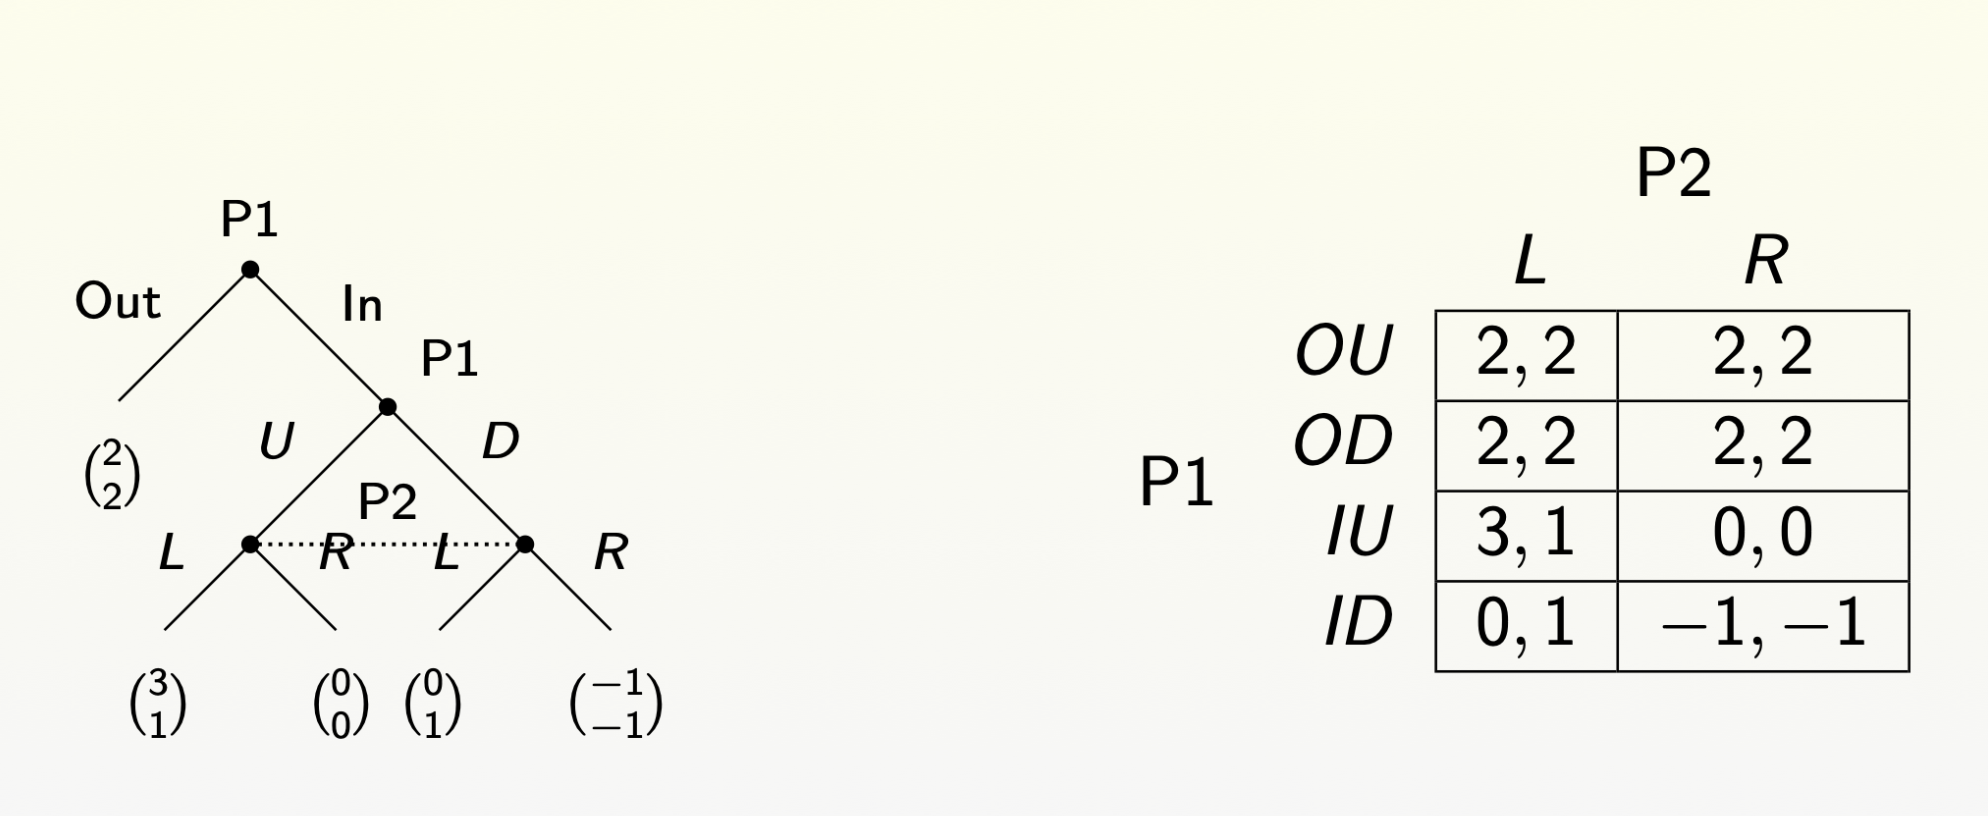
\includegraphics[scale=0.2]{BS.png}
    \caption{Example}
    \label{}
\end{figure}
In this example, a mixed strategy of the P1 can be represented by a probability distribution over $\{OU,OD,IU,ID\}$. To replicate mixed strategy, we can use \textbf{behavioral strategy} that an agent's (probabilistic) choice at each node is independent of his/her choices at other nodes.
\begin{example}
    \begin{enumerate}
        \item Mixed Strategy: $OU$ with probability $\frac{1}{2}$ and $ID$ with probability $\frac{1}{2}$.
        \item Behavioral Strategy: play $O$ and $I$ with prob $\frac{1}{2}$ each at $h = \emptyset$;
        and then $D$ with prob $1$ at history $h = I$.
    \end{enumerate}
\end{example}

\begin{definition}[Behavioral Strategy]
    %\normalfont
    A \textbf{behavioral strategy} for player $i$ is a function that maps histories $h \in H_i$ into probability distributions over $A_i(h)$,
    $$\sigma_i(h)\in\Delta(A_i(h))$$
\end{definition}

A profile of behavioral strategies, $\sigma=\{\sigma_i:i\in N\}$, includes a probability distribution over $Z$. So does a profile of mixed strategies. Then $u_i(\sigma)$ is the expected payoff.

\begin{theorem}[Outcome Equivalent]
    Behavioral and mixed strategies are ``outcome equivalent'' in games of \textbf{perfect recall}.
\end{theorem}
Without perfect recall, behavioral and mixed strategies are not equivalent.


\subsection{Subgame Perfect Equilibrium}
\begin{definition}
    %\normalfont
    A strategy profile $\sigma^*$ is a \textbf{Nash equilibrium} if, for all $i$,
    \begin{enumerate}
        \item $\sigma_i^*$ is the best response to beliefs $\mu_i$,
        \item $\mu_i$ coincides with $\sigma_{-i}^*$.
    \end{enumerate}
\end{definition}
When $s$ is a pure-strategy Nash eq. $h(s)$ is the equilibrium path of $s$.

\begin{definition}
%\normalfont
A subgame of an extensive-form game $G=\{N,A,H,Z,P,O,o,\succ_{n\in N}\}$ is a game that starts after a given finite history $h \in H$.

Formally, the subgame $\Gamma(h)$ associated with $h=(h_1,...,h_n)\in H$ is $\Gamma(h)=\left(N,A,H_h,P_h,\{u_{i,h}\}_{i\in N}\right)$, where $H_h=\{(a_1,a_2,...):(h_1,...,h_n,a_1,a_2,...)\in H\}$. $P_h(h')=P(hh')$ for all non-terminal $h'\in H_h$, and $u_{i,h}=u_i(hh')$ for any terminal $h'\in H$.
\end{definition}
A behavioral strategy $\sigma_i$ of $i$ in $\Gamma$ defines a behavioral strategy $\sigma_i(\cdot|h)$ of $\Gamma(h)$ by $\sigma_i(h'|h)=\sigma_i(hh')$.



\begin{definition}[Subgame Perfect Equilibrium]
    %\normalfont
    A \textbf{subgame perfect equilibrium}[SPNE/SPE] of $\Gamma$ is a strategy profile $\sigma^*$ such that for every subgame $\Gamma(h)$ it holds that $\sigma^*$ (more precisely, its restriction to $H_h$) is a Nash equilibrium of $\Gamma(h)$.
\end{definition}
Over time $t=1,...,T$, the set of actions is $A^T$.
\begin{lemma}
    $\sigma^*$ is a SPNE \underline{iff} its restriction $\sigma^*(\cdot|h)$ is SPNE of $\Gamma(h)$, for all subgames $\Gamma(h)$.
\end{lemma}

\subsection{Infinite Horizon Games}
\begin{definition}[Finite Horizon]
    %\normalfont
    An extensive-form game has a \textbf{finite horizon} if there is a bound on the length of any history in $Z$.
\end{definition}
In these games, SPNE can be found through ``generalized backwards induction.''

\begin{definition}[Continuous At Infinity Utility Function]
    %\normalfont
    A utility function $v:A^T \rightarrow \mathbb{R}$ is \textbf{continuous at infinity} if
    \begin{equation}
        \begin{aligned}
            \lim_{t \rightarrow \infty}\sup\{|v(\hat{h})-v(h)|:h,\hat{h}\in A^T\}=0
        \end{aligned}
        \nonumber
    \end{equation}
    That is, eventually, a negligible effect on utility.
\end{definition}

\begin{definition}[Discounted Utility]
%\normalfont
We focus on additively separable models with a sub-utility $u:A \rightarrow \mathbb{R}$ that is the same for each $t$. We model a \textbf{discounted utility} by assuming a discount factor $\delta\in[0,1)$:
\begin{equation}
    \begin{aligned}
        v(a_1,...)=(1-\delta)\sum_{t=1}^\infty \delta^{t-1}u(a_t)
    \end{aligned}
    \nonumber
\end{equation}
\end{definition}
Can think of $\delta$ as the probability that the game will go on for another period, and $1-\delta$ the prob that the game will end.

“Ending” events are independent: A geometric distribution.

The probability that the game ends at time $t$ is $(1 - \delta)\delta^{t-1}$ and $\sum(1-\delta)\delta^t u(a_t)$ becomes expected utility.

\begin{proposition}
    $v(a_1,...)=(1-\delta)\sum_{t=1}^\infty \delta^{t-1}u(a_t)$ is continuous at infinity.
\end{proposition}


\subsection{Repeated Games}
Let $G_0=\left(N,\{A_i:i\in N\},\{u_i:i\in N\}\right)$ be a normal-form game. We let $A=\Pi_{i\in N}A_i$. We only consider games in which $A$ is compact and each $u_i$ is continuous.

Let $T$ be the number of periods (or repetitions) of the repeated game. $T$ can be either finite or infinite. $G_0$ is the stage game.

\begin{definition}[Repeated Game]
    %\normalfont
    A $T$-repeated, $\delta$-discounted, game of $G_0$ is an extensive form game $\Gamma=\left(N,A,H,P,\{u_i\}_{i\in N},\delta\right)$, where
    \begin{enumerate}
        \item $P(h)=N$ for all $h\in H/Z$.
        \item The set of histories $H$ has terminal histories $Z=A^T$; recall that $Z$
        uniquely determines $H$ as the set of all prefixes of $Z$.
        \item $v_i:Z \rightarrow \mathbb{R}$ is a payoff function of the form
        \begin{equation}
            \begin{aligned}
                v((a_t)_{t=1}^T)=\left\{\begin{matrix}
                    (1-\delta)\sum_{t=1}^\infty \delta^{t-1}u(a_t),&\delta\in(0,1)\\
                    \sum_{t=1}^T u_i(a_t),&\delta=1
                \end{matrix}\right.
            \end{aligned}
            \nonumber
        \end{equation}
    \end{enumerate}
\end{definition}
Given a strategy profile $s$, we obtain a terminal history $z \in Z$, and (abusing notation) write $v_i(s)$ for $v_i(z)$.

We call $(v_1(s),...,v_n(s))$ the \textbf{payoff profile} associated with $s$.

%The set $\mathcal{F}=\{(u_1(v),...,u_n(v)):v\in\Delta(A)\}$ is the set of \textbf{feasible payoffs}, which is a convex hull of $\{(u_1(a),...,u_n(a)):a\in A\}$.

\begin{definition}[(Profitable) One-Stage Deviation]
    %\normalfont
    A \textbf{one-stage deviation} from $\sigma$ by $i$ is a strategy $\sigma'_i$ that coincides with $\sigma_i$ everywhere except at a single history.\\
    A \textbf{profitable one-stage deviation} from $\sigma$ by $i$ is a strategy $\sigma'_i$ that coincides with $\sigma_i$ at a single history $h$, and for which $v_i(\sigma'_i,\sigma_{-i}|h)>v_i(\sigma_i,\sigma_{-i}|h)$.
\end{definition}

\begin{proposition}[SPNE$\Leftrightarrow$No Profitable One-Stage Deviation]
    Let $\Gamma$ be a discounted, infinitely repeated game. Then a strategy-profile is a SPNE of $\Gamma$ \underline{iff} no player has a profitable one-stage deviation.
\end{proposition}

\begin{corollary}[NE$\Rightarrow$SPNE]
    If $s$ is a pure-strategy Nash equilibrium of $G_0$, then the strategy profile in which each player chooses $s_i$ after any history, is a SPNE of infinitely-repeated discounted $G_0$.
\end{corollary}

\begin{proposition}[Nash Reversion Folk Theorem]
    Let $\sigma$ be a Nash equilibrium of the finite stage game $G_0$. Let $v$ be a feasible payoff profile s.t. $u_i(\sigma) < v_i$ for all players $i$. Then there is $\underline{\delta}$ s.t. if $\delta\geq \underline{\delta}$ then there exists a SPNE of infinitely repeated $G_0$ with discount factor $\delta$ in which players' equilibrium payoffs is the profile $v$.
\end{proposition}
No Nash equilibrium that has higher payoffs for all players than Nash equilibrium can be obtained with relatively high discount factor in an infinite game.


\section{Refinement}
\subsection{Trembling-hand Perfect Equilibrium}
\begin{definition}[$\epsilon$-Constrained Equilibrium]
    An \textbf{$\epsilon$-constrained equilibrium} of a strategic form game is a mixed strategy profile $\sigma^\epsilon$ such that there exists $\bar{\epsilon}: \bigcup_{i \in I} S_i \rightarrow(0, \epsilon)$ such that for each player $i$,
    \begin{equation}
        \begin{aligned}
            \sigma^\epsilon_i\in\argmax_{\sigma_i \textnormal{ s.t. }\sigma_i(s_i)\geq \bar{\epsilon}(s_i)} u_i(\sigma_i,\sigma^\epsilon_{-i})
        \end{aligned}
        \nonumber
    \end{equation}
\end{definition}


\begin{definition}[Trembling-hand Perfect Equilibrium]
    A strategy profile $\sigma$ is a \textbf{trembling-hand perfect equilibrium} of a strategic form game if it is a limit of $\epsilon$-constrained equilibria as $\epsilon \rightarrow 0$.
\end{definition}

\begin{note}
    Trembling-hand perfect equilibrium implies a SPE, while a SPE is not always a trembling-hand perfect equilibrium.
\end{note}

This doesn't imply backward induction. (We do not rationalize the ``trembling-hand''.)


\subsection{Forward Induction: Burning Money (Ben-Polath and Dekel, 1992)}
Consider a game as following:
\begin{center}
    \begin{tabular}{ccc}
        \hline
            &$A_2$ &$B_2$\\
        \hline
            $A_1$& 9,6 & 0,4\\
            $B_1$& 4,0 & 6,9\\
        \hline
    \end{tabular}
\end{center}
Except the actions, the Player 1 can choose to Burn or Not Burn (i.e., lose $2.5$ units of utility), and the Player 2 can see the Player 1's action.

There are four possible strategies of Player 1:
\begin{enumerate}[(S1).]
    \item Burn and $A_1$
    \item Burn and $B_1$
    \item Not Burn and $A_1$
    \item Not Burn and $B_1$
\end{enumerate}
The potential payoffs of playing (S2) are $1.5$ and $3.5$, which is dominated by playing (S4). Then, if the Player 1 chooses Burn, he must play (S1). Thus, the Player 2 plays $A_2$, which gives $(6.5,6)$. Therefore, the Player 1 chooses Burn (i.e., (S1)) can dominate (S4). Now, we only remain two possible strategies of Player 1, (S1) and (S3). (S1) is dominated by (S3), so (S3) is the optimal strategy of Player 1.

\section{Signaling Game}
\subsection{Canonical Game}
\begin{definition}[Canonical Game]
    %\normalfont
    \begin{enumerate}
        \item There are two players: $\mathbf{S}$ (sender) and $\mathbf{R}$ (receiver).
        \item $\mathbf{S}$ holds more information than $\mathbf{R}$: the value of some random variable $t$ with support $\mathcal{T}$. (We say that $t$ is the \textbf{type} of $\mathbf{S}$)
        \item Prior belief of $\mathbf{R}$ concerning $t$ are given by a probability distribution $\rho$ over $\mathcal{T}$ (common knowledge)
        \item $\mathbf{S}$ sends a \textbf{signal $s\in \mathcal{S}$} to $\mathbf{R}$ drawn from a signal set $\mathcal{S}$.
        \item $\mathbf{R}$ receives this signal, and then takes an \textbf{action} $a\in \mathcal{A}$ drawn from a set $\mathcal{A}$ (which could depend on the signal $s$ that is sent).
        \item $\mathbf{S}$'s payoff is given by a function $u: \mathcal{T}\times \mathcal{S} \times \mathcal{A} \rightarrow \mathbb{R}$ and $\mathbf{R}$'s payoff is given by a function $v: \mathcal{T}\times \mathcal{S} \times \mathcal{A} \rightarrow \mathbb{R}$.
    \end{enumerate}
\end{definition}

\subsection{Nash Equilibrium}
\begin{definition}[Strategy]
    %\normalfont
    A \textbf{behavior strategy} for $\mathbf{S}$ is given by a function $\sigma: \mathcal{T}\times\mathcal{S} \rightarrow [0,1]$ such that $\sum_s \sigma(t,s)$ for each $t$.\\
    A \textbf{behavior strategy} for $\mathbf{R}$ is given by a function $\alpha: \mathcal{S}\times\mathcal{A} \rightarrow [0,1]$ such that $\sum_a \alpha(s,a)$ for each $t$.
\end{definition}

\begin{definition}[Nash Equilibrium]
    %\normalfont
    Behavior strategies $\alpha$ and $\sigma$ form a \textbf{Nash equilibrium} if and only if
    \begin{enumerate}
        \item For all $t\in \mathcal{T}$,
        \begin{center}
            $\sigma(t,s)>0$ implies $\sum_a \alpha(s,a)u(t,s,a) = \max_{s'\in \mathcal{S}}\left(\sum_a \alpha(s',a)u(t,s',a)\right)$
        \end{center}
        \item For each $s\in \mathcal{S}$ such that $\sum_{t}\sigma(t,s)\rho(t)>0$,
        \begin{center}
            $\alpha(s,a)>0$ implies $\sum_{t}\mu(t;s)v(t,s,a) = \max_{a'}\sum_{t}\mu(t;s)v(t,s,a')$
        \end{center}
        where $\mu(t;s)$ is the $\mathbb{R}$'s posterior belief about $t$ given $s$, $\mu(t;s)=\frac{\sigma(t,s)\rho(t)}{\sum_{t'}\sigma(t',s)\rho(t')}$ if $\sum_t\sigma(t,s)\rho(t)>0$ and $\mu(t;s)=0$ otherwise.
    \end{enumerate}
\end{definition}

\begin{definition}[Separating \& Pooling Equilibrium]
    %\normalfont
    An equilibrium $(\sigma,\alpha)$ is called a \textbf{separating} equilibrium if each type $t$ sends different signals; i.e., the set $\mathcal{S}$ can be partitioned into (disjoint) sets $\{\mathcal{S}_t; t\in \mathcal{S}\}$ such that $\sigma(t, \mathcal{S}_t) = 1$. An equilibrium $(\sigma,\alpha)$ is called a \textbf{pooling} equilibrium if there is a single signal $s^*$ that is sent by all types; i.e., $\sigma(t, s^*) = 1$ for all $t\in \mathcal{T}$.
\end{definition}


\subsection{Single-crossing}

\subsubsection{Situation over real line}
Consider the situation that $\mathcal{T},\mathcal{S},\mathcal{A}\subseteq \mathbb{R}$ and $\geq$ is the usual "greater than or equal to" relationship.

\begin{enumerate}
    \item We let $\Delta \mathcal{A}$ denote the set of probability distributions on $\mathcal{A}$.
    \item For each $s\in \mathcal{S}$ and $\mathcal{T}'\subseteq \mathcal{T}$, we let $\Delta\mathcal{A}(s,T')$ be the set of mixed strategies that are the best responses by $\mathbf{R}$ to $s\in \mathcal{S}$ for some probability distribution with support $\mathcal{T}'$.
    \item For $\alpha\in \Delta\mathcal{A}$, we write $u(t,s,\alpha)\triangleq \sum_{a\in \mathcal{A}}u(t,s,a)\alpha(a)$.
\end{enumerate}

\begin{definition}[Single-crossing]
    %\normalfont
    The data of the game are said to satisfy the \textbf{single-crossing property} if the following holds: If $t\in \mathcal{T}$, $(s,\alpha)\in \mathcal{S}\times \Delta\mathcal{A}$ and $(s',\alpha')\in \mathcal{S}\times \Delta\mathcal{A}$ are such that $\alpha\in \Delta\mathcal{A}(s,\mathcal{T})$, $\alpha'\in \Delta\mathcal{A}(s',\mathcal{T})$, $s>s'$ and $u(t,s,\alpha)\geq u(t,s',\alpha')$, then for all $t'\in T$ such that $t'>t$, $u(t',s,\alpha)\geq u(t',s',\alpha')$.
\end{definition}

\section{Adverse Selection}
Consider a labor market that has many identical firms. In competitive equilibrium, firms' profits are $0$. Firms are price (wage) takers, risk-neutral, and CRS. There are continuum of workers with productivity levels $\theta\in\left[\underline{\theta},\overline{\theta}\right]$ (Assume workers work if it is indifferent for them between employment and non-employment).
\begin{enumerate}
    \item $\theta\sim F$, $F(\cdot)$ is a c.d.f. over $\left[\underline{\theta},\overline{\theta}\right]$.
    \item $N$ is the total mass of workers.
    \item Type $\theta$ worker has a reservation utility $r(\theta)$.
\end{enumerate}

\begin{enumerate}[$\circ$]
    \item Suppose the competitive equilibrium wages are $\theta=w^*(\theta)$.
    \item An allocation is denoted by $I:\left[\underline{\theta},\overline{\theta}\right] \rightarrow \{0,1\}$, where $I(\theta)=0$ denotes $\theta$ is unemployed and $I(\theta)=1$ denotes $\theta$ is employed.
    \item Aggregate welfare = sum of utilities of all participants
    \begin{equation}
        \begin{aligned}
            =N\int_{\underline{\theta}}^{\overline{\theta}} \left[I(\theta)\times\theta+[1-I(\theta)]r(\theta)\right]dF(\theta)
        \end{aligned}
        \nonumber
    \end{equation}
    Then we have the optimal allocation satisfies
    \begin{equation}
        \begin{aligned}
            I^*(\theta)\left\{\begin{matrix}
                =1,&\theta>r(\theta)\\
                \in\{0,1\}&\theta=r(\theta)\\
                =0,&\theta<r(\theta)
            \end{matrix}\right.
        \end{aligned}
        \nonumber
    \end{equation}
\end{enumerate}
In the asymmetric information case,
\begin{definition}
%\normalfont
$w$ is CE wage if $w=\mathbb{E}[\theta|r(\theta)\leq w]$.
\end{definition}

\subsection{Adverse Selection}
\begin{assumption}
    \begin{enumerate}[({A}1).]
        \item $r$ is strictly increasing in $\theta$.
        \item $F(\cdot)$ has a strictly positive density, $F(\theta)>0, \forall \theta\in \left[\underline{\theta},\overline{\theta}\right]$.
        \item $r(\theta)\leq\theta$ (outside option is worse than productivity, i.e., full employment is optimal).
    \end{enumerate}
\end{assumption}

\begin{lemma}
    Under A1-A3, $\Phi(w):=\mathbb{E}[\theta|r(\theta)\leq w]$ is well-defined, continuous, and non-decreasing.
\end{lemma}

Hence, there exists underemployment, which makes $1^{st}$ welfare theorem fails. There may exist multiple CEs, where the one with the highest wage Pareto dominates others.

\begin{example}
    Suppose $\theta\in[0,2]$, $F(\theta)=\frac{\theta}{2}$, $f(\theta)=\frac{1}{2}$, $r(\theta)=\alpha\theta,\alpha\in(0,1)$.
    \begin{equation}
        \begin{aligned}
            \mathbb{E}[\theta|r(\theta)\leq w]=\mathbb{E}\left[\theta|\theta \leq \frac{w}{\alpha}\right]=\left\{\begin{matrix}
                1,&w\geq 2\alpha\\
                \frac{1}{F\left(\frac{w}{\alpha}\right)}\int_0^{\frac{w}{\alpha}}\theta f(\theta)d\theta=\frac{w}{2\alpha},&w\leq 2\alpha
            \end{matrix}\right.
        \end{aligned}
        \nonumber
    \end{equation}
    CEs are given by $\mathbb{E}[\theta|r(\theta)\leq w]=w$. $w^*=0$ is always CE and $w^*=1$ is CE if $\alpha\leq\frac{1}{2}$.
\end{example}

\subsection{Game Theoretical Approach}
\begin{enumerate}
    \item Suppose there are two firms setting wages simultaneously.
    \item Workers observe the wages in stage 1 and make an employment decision.
\end{enumerate}
Let $W^*$ be the set of CE wages and $w^*:=\max W^*$.
\begin{lemma}\label{lemma:ad_l2}
    $\forall w'\in\left(w^*,\overline{\theta}\right]$: $\mathbb{E}[\theta|r(\theta)\leq w']<w'$.
\end{lemma}
\begin{proof}
    Suppose by the contradiction that $\exists w'\in \left(w^*,\overline{\theta}\right]$ s.t. $\mathbb{E}[\theta|r(\theta)\leq w']\geq w'$. Since $\mathbb{E}[\theta|r(\theta)\leq \overline{\theta}]<\overline{\theta}$, there must exist a $w''\in [w',\overline{\theta})$ s.t. $\mathbb{E}[\theta|r(\theta)\leq w'']=w''$ by intermediate value theorem, which contradicts to the definition of $w^*$.
\end{proof}

\begin{proposition}
    \begin{enumerate}[(i).]
        \item If $w^*>r(\underline{\theta})$ and $\exists \epsilon>0$ s.t. $\mathbb{E}[\theta|r(\theta)\leq w']>w',\forall w'\in \left(w^*-\epsilon,w^*\right)$. Then, there is a unique SPE where both firms set wage $=w^*$.
        \item If $w^*=r(\underline{\theta})$ (complete market shutdown at $w^*$), there are multiple SPE that all give the same outcome as complete market shutdown where both firms set wage $=w^*$.
    \end{enumerate}
\end{proposition}
\begin{proof}
    \begin{lemma}\label{lemma:p1}
        In all SPE, firms make zero profits.
    \end{lemma}
    \begin{proof}
        Suppose not, i.e., at least one firm makes strictly positive profits. Then, the total profits of firms $1\&2$, $$\Pi=M(\bar{w})\left[\mathbb{E}[\theta|r(\theta)\leq\bar{w}]-\bar{w}\right]>0$$
        where $\bar{w}$ is the max wage set by the two firms and $M(\bar{w})$ is the mass of workers willing to work at $\bar{w}$. At least one firm, $i$, makes profit $\leq\frac{\Pi}{2}$. Then, $i$'s profits from setting $\bar{w}+\delta$, with $\delta \rightarrow 0^+$, is higher:
        \begin{equation}
            \begin{aligned}
                &M(\bar{w}+\delta)\left[\mathbb{E}[\theta|r(\theta)\leq\bar{w}+\delta]-\bar{w}-+\delta\right]\\
                \geq &M(\bar{w})\left[\mathbb{E}[\theta|r(\theta)\leq\bar{w}+\delta]-\bar{w}-+\delta\right] \rightarrow \Pi \textnormal{ as }\delta \rightarrow 0
            \end{aligned}
            \nonumber
        \end{equation}
        Hence, the $i$ has incentive to deviate.
    \end{proof}
    \begin{lemma}\label{lemma:p2}
        In all SPE, firm $i$ sets $w_i\leq w^*, i\in\{1,2\}$.
    \end{lemma}
    \begin{proof}
        Directly given by Lemma \ref{lemma:ad_l2} and Lemma \ref{lemma:p1}.
    \end{proof}
    \begin{enumerate}[(i):]
        \item In SPE, no firm $i$ sets $w_i<w^*$: suppose $w_i<w^*$ and let $j\neq i$, take any $w'_j$ s.t. $w'_j\in\left(w_i,w^*\right)$ and $w'_j>w^*-\epsilon$. Then, $j$ gets profit: $M(w'_j)\left[\mathbb{E}[\theta|r(\theta)\leq w'_j]-w'_j\right]>0$ (by Case (i)'s conditions).
        \item By Lemma \ref{lemma:p2}, both firms set $w_i\leq w^*=r(\underline{\theta})$. Check that $\{(w_1,w_2):w_1,w_2\leq w^*\}$ is SPE wage profiles.
    \end{enumerate}
\end{proof}

\subsection{Planner Intervention}
Planner can't observe the true type $\theta$.

The planner's tools:
\begin{enumerate}
    \item Take over the firms.
    \item $w_e$, employment wage.
    \item $w_u$, unemployment wage.
\end{enumerate}
s.t. budget balanced.

\begin{definition}[Constrained Efficient]
    %\normalfont
    A CE $w$ is \textbf{constrained efficient} if it cannot be Pareto improved upon by an intervention by the planner.
\end{definition}

\begin{proposition}[$w^*:=\max W^*$ is constrained efficient]
    Let $W^*$ be the set of CE wages. $w^*:=\max W^*$ is constrained efficient.
\end{proposition}
\begin{proof}
    Note that both firms are making zero profits by the Lemma \ref{lemma:p1}. Any CE wage $w\neq w^*$ can be Pareto improved by $\{w_e=w^*,w_u=0\}$. Then, we prove $w^*$ can't be Pareto improved.
    \begin{enumerate}
        \item Case 1: if $w^*$ gives full-employment in CE, then $w^*$ is Pareto efficient.
        \item Case 1: suppose $w^*$ doesn't give full-employment in CE.
        
        Consider taking an intervention $w_e\&w_u$. Then, $\{\theta:r(\theta)+w_u\leq w_e\}=[\underline{\theta},\hat{\theta}]$ for some $\hat{\theta}\in[\underline{\theta},\overline{\theta}]$ such that
        \begin{equation}
            \begin{aligned}
                r(\hat{\theta})+w_u=w_e
            \end{aligned}
            \label{con:1}
        \end{equation}
        The budget balanced gives
        \begin{equation}
            \begin{aligned}
                w_e F(\hat{\theta})+w_u (1-F(\hat{\theta}))=\int_{\underline{\theta}}^{\hat{\theta}}\theta d F(\theta)
            \end{aligned}
            \label{con:2}
        \end{equation}
        Plug \eqref{con:1} into \eqref{con:2}:
        \begin{equation}
            \begin{aligned}
                \left\{\begin{matrix}
                    &w_u(\hat{\theta})=\int_{\underline{\theta}}^{\hat{\theta}}\theta d F(\theta)-r(\hat{\theta})F(\hat{\theta})=F(\hat{\theta})\left(\mathbb{E}[\theta|\theta\leq\hat{\theta}]-r(\hat{\theta})\right)\\
                    &w_e(\hat{\theta})=\int_{\underline{\theta}}^{\hat{\theta}}\theta d F(\theta)+r(\hat{\theta})(1-F(\hat{\theta}))
                \end{matrix}\right.
            \end{aligned}
            \nonumber
        \end{equation}
        Let $\theta^*$ be s.t. $r(\theta^*)=w^*$. Because $w^*$ is a CE price, $\mathbb{E}[\theta|\theta\leq\theta^*]=r(\theta^*)=w^*$. So, CE with $w^*$ can be implemented by $w_u(\theta^*)=0$ and $w_e(\theta^*)=w^*$.
        \begin{enumerate}
            \item If $\hat{\theta}<\theta^*$. $\underline{\theta}$ is worse off under the intervention since $w_e(\hat{\theta})<w^*$.
            \item If $\hat{\theta}>\theta^*$. $\overline{\theta}$ is worse off under the intervention since $w_u(\hat{\theta})=F(\hat{\theta})\left(\mathbb{E}[\theta|\theta\leq\hat{\theta}]-r(\hat{\theta})\right)<0$ by the Lemma \ref{lemma:ad_l2}
        \end{enumerate}
    \end{enumerate}
\end{proof}


\subsection{Signaling}\label{sec:signaling}
Suppose the worker $\theta\in[\underline{\theta},\overline{\theta}]$ can properly and costlessly reveal his type to the firms. Then,
\begin{lemma}
    All workers revel their types.
\end{lemma}
\paragraph*{Spence's Job Market Signaling Model} One worker has productivity $\theta\in\{\theta_L,\theta_H\}$ with $P(\theta_H)=\lambda$. The worker signal through his education with cost $e>0$. The education doesn't change his productivity. The payoff of the worker is the wage minus the cost:
\begin{equation}
    \begin{aligned}
        u(w,e|\theta)=w-c(e,\theta)
    \end{aligned}
    \nonumber
\end{equation}
where $c(0,\theta)=0,c_e(e,\theta):=\frac{\partial c(e,\theta)}{\partial e}>0, c_\theta(e,\theta):=\frac{\partial c(e,\theta)}{\partial \theta}<0$, and $c_{e\theta}(e,\theta):=\frac{\partial^2 c(e,\theta)}{\partial e\partial \theta}<0$ (Single-Crossing Property, the difference $c(e,\theta_L)-c(e,\theta_H)$ is increasing in $e$ (i.e., $c_e(e,\theta_L)-c_e(e,\theta_H)>0$), which means if $c(e,\theta_L)$ and $c(e,\theta_H)$ intersect as functions of $e$, they only intersect at one time.)
\begin{enumerate}[]
    \item \underline{Stage 0}: Nature chooses the $\theta\in\{\theta_L,\theta_H\}$ with $P(\theta_H)=\lambda$.
    \item \underline{Stage 1}: The worker learns $\theta$ and chooses $e(\theta)\geq 0$.
    \item \underline{Stage 2}: Firms observe $e(\theta)$. Then, they simultaneously make wage offers $w_1$ and $w_2$.
    \item \underline{Stage 3}: The worker observes $w_1,w_2$ and makes employment decision.
\end{enumerate}
Let $r(\theta_L)$ and $r(\theta_H)=0$. Let $\mu(e)\in[0,1]$ be the probability that in the beginning of stage 2, firms think that the worker is $\theta_H$ type with probability $\mu(e)$ when observing $e$. The corresponding expected productivity (the highest wage) that the firm can pay is
\begin{equation}
    \begin{aligned}
        w(e)=\mu(e)\theta_H+(1-\mu(e))\theta_L
    \end{aligned}
    \nonumber
\end{equation}
In stage 2, both firm will set $w(e)$ (complete competition).

\begin{definition}[Perfect Bayesian Equilibrium]
    %\normalfont
    A PBE is a strategy profile ($e^*(\theta_L)$, $e^*(\theta_H)$, $w^*_1: \mathbb{R}_+ \rightarrow \mathbb{R}$, $w^*_2: \mathbb{R}_+ \rightarrow \mathbb{R}$), and a belief $\mu^*: \mathbb{R} \rightarrow [0,1]$ such that
    \begin{enumerate}
        \item $\forall \theta\in\{\theta_L,\theta_H\}$, the worker strategy optimal given firm strategies.
        \item The belief $\mu^*(e)$ is derived from $\lambda, e^*(\theta_L), e^*(\theta_H)$ via Bayes' rule whenever possibly (on the equilibrium path). Outside the equilibrium path the belief $\mu^*(e)$ is arbitrarily.
        \item Firms offer wages that form a NE of the stage 2 game, where their belief $\mu^*(e)$ about their workers' type. (sequential rationality).
    \end{enumerate}
\end{definition}
We simplify the game by backward induction:
\begin{enumerate}
    \item \underline{Stage 3}: The worker chooses the highest wage off if it is $\geq 0$.
    \item \underline{Stage 2}: After observing $e(\theta)$, firms chooses the wage as the expected productivity in NE,
    \begin{equation}
        \begin{aligned}
            w^*(e)=\mu^*(e)\theta_H+(1-\mu^*(e))\theta_L
        \end{aligned}
        \nonumber
    \end{equation}
    because it is a Bertrend competition.
\end{enumerate}
\paragraph*{Separating Equilibrium}
In separating equilibrium, $e^*(\theta_L)\neq e^*(\theta_H)$.
\begin{lemma}
    In any separating PBE, $w^*(e^*(\theta))=\theta, \forall \theta\in\{\theta_L,\theta_H\}$.
\end{lemma}
\begin{proof}
    By Bayes' rule, after firm observe $e^*(\theta_L)$, $\mu^*(e^*(\theta_L))=0$. Then, $w^*(e^*(\theta_L))=\theta_L$. ($e^*(\theta_H)$ is similar.)
\end{proof}

\begin{lemma}
    In separating PBE, low type always chooses zero education, $\theta^*(\theta_L)=0$.
\end{lemma}
\begin{proof}
    If not, the low type worker always has profitable deviation, $\theta^*(\theta_L)=0$.
\end{proof}

\begin{lemma}
    Define $\underline{e}$ and $\overline{e}$ such that
    \begin{enumerate}
        \item $\theta_L=\theta_H-c(\underline{e},\theta_L)$ (the lowest effort can prevent the low type from mimicking high type) and
        \item $\theta_L=\theta_H-c(\overline{e},\theta_H)$ (the highest effort can prevent the high type from pooling with low type).
    \end{enumerate}
    Then, in all separating PBEs, $e\in \left[\underline{e},\overline{e}\right]$.\\
    Conversely, $\forall \hat{e}\in \left[\underline{e},\overline{e}\right]$, there is a separating PBE where $e^*(\theta_H)=\hat{e}$.
\end{lemma}
These different PBEs are Pareto ranked. High type prefers the PBE with a lower $e$ (the best is the one with $e^*(\theta_H)=\underline{e}$.)

\paragraph*{Pooling PBE}
$e^*(\theta)=e^*,\theta\in\{\theta_L,\theta_H\}$, $\mu^*(e^*)=\lambda$, and $w^*(e^*)=\mathbb{E}[\theta]$.

\begin{lemma}
    Define $e'$ by $\theta_L=\mathbb{E}[\theta]-c(e',\theta_L)$ (the highest effort can prevent the low type from choosing $e=0$ and get $w=\theta_L$.)\\
    Then, for all pooling PBE, $e^*(\theta_L)=e^*(\theta_H)=e^*\in[0,e']$. Conversely, for all $\hat{e}\in [0,e']$, there is a pooling PBE with $e^*=\hat{e}$.
\end{lemma}


\subsection{Cho-Kreps Intuitive Criterion}
\begin{definition}[Equilibrium Dominated Message]
    %\normalfont
    A message is \textbf{equilibrium dominated} for a type if the type must do strictly worse by sending the message than it does in equilibrium (i.e., payoff in eq. is strictly better than maximum payoff from deviating).
\end{definition}

\begin{definition}[Cho-Kreps Intuitive Criterion]
    %\normalfont
    If an information set is off the eq. path and a message is eq. dominated for a type, then beliefs should assign zero probability to the message coming from that type (if possible).
\end{definition}

Fix a PBE $e^*(\theta), \theta\in\{\theta_L,\theta_H\}, \mu^*(\cdot)$ (We know $w_1^*(e)=w_2^*(e)=\mu(e)\theta_H+(1-\mu(e))\theta_L$). Let $u^*(\theta),\theta\in\{\theta_L,\theta_H\}$ be the PBE utility of the type $\theta$ worker.

The criterion requires the (off-path) belief $\mu^*(e):=P(\tilde{\theta}=\theta_H|e)=1-P(\tilde{\theta}=\theta_L|e)$ satisfies $$P(\tilde{\theta}=\theta|e)=0,\forall e,\theta$$ such that
\begin{enumerate}
    \item $u^*(\theta)>\max_{w\in[\underline{\theta},\overline{\theta}]}[w-c(e,\theta)]$
    \item $\exists \theta'$ s.t. $u^*(\theta')\leq \max_{w\in[\underline{\theta},\overline{\theta}]}[w-c(e,\theta')]$ (make sure the sum of beliefs given $e$ is nonzero.)
\end{enumerate}
In this application, the only PBE that survives Intuitive Criterion is the best separating PBE, $e^*(\theta_H)=\underline{e}$ (the lowest effort).



\subsection{Grossman-Perry-Farrell Equilibrium}
For the equilibrium refinement, we can also introduce the Grossman-Perry-Farrell equilibrium based on the perfect sequential equilibrium (grossman1986sequential) and the neologism-proof equilibrium (farrell1993meaning). We formally define the Grossman-Perry-Farrell equilibrium by ruling out the self-signaling sets in Perfect Bayesian Equilibrium (bertomeu2018verifiable,glode2018voluntary).

A binary example is given as follows:
\begin{definition}[Grossman-Perry-Farrell Equilibrium (GPFE)]
	A pure-strategy perfect Bayesian equilibrium $(p^*_L,p^*_H,b^*(\cdot))$ is a ``Grossman-Perry-Farrell equilibrium'' (GPFE) if there does not exist a self-signaling set, which is defined by a set $\chi\subseteq\{L,H\}$ such that there exists a price $p'$ such that
	\begin{equation}
		\begin{aligned}
			\chi=\{j\in\{L,H\}:U(p',\mu_\chi)>U(p_j^*,b^*(p_j^*))\},
		\end{aligned}
		\nonumber
	\end{equation}
	where $\mu_\chi=\frac{q_L\rho_e\mathbf{1}_{L\in\chi}+q_H(1-\rho_e)\mathbf{1}_{H\in\chi}}{\rho_e\mathbf{1}_{L\in\chi}+(1-\rho_e)\mathbf{1}_{H\in\chi}}$ is the average quality of types in $\chi$ based on the relative prior probabilities.
\end{definition}

\begin{note}
    The GPFE is a strong refinement of PBE that may lead to no equilibrium exists.
\end{note}

\subsection{Screening Model}
Workers can undertake a contractible/observable task level $t\geq 0$. The utility of a worker is defined by $u(w,t,\theta):=w-c(t,\theta)$, where $c(\cdot,\cdot)$ satisfies the same assumption as in signaling model \ref{sec:signaling}.

The Game follows
\begin{enumerate}[]
    \item \underline{Stage 1}: Two firms simultaneously determine sets of contracts, $(w,t)$.
    \item \underline{Stage 2}: The worker observes all offer contracts and makes employment decision.
    (If indifference, choose lower task contract, favor employment over unemployment. If contracts of firms are indifferent, choose each with probability 1/2.)
\end{enumerate}

The null contract is $(w,t)=(0,0)$. Assume WLOG at stage 1, each firm appears a non-empty set of contracts.

\subsubsection*{Perfect Information}
\begin{proposition}[Perfect Information]
    If firms can observe the worker types, then in SPE firms make zero profit and type $\theta_i$ worker signs $(w^*_i,t^*_i)=(\theta_i,0)$.
\end{proposition}
\begin{proof}
    \begin{claim}
        Firms make zero profits from this contract.
    \end{claim}
    \begin{proof}
        Suppose not,
    \begin{enumerate}[$\circ$]
        \item $w^*_i>\theta_i$ $\Rightarrow$ negative profits, firms benefit from offering null contract.
        \item $w^*_i<\theta_i$ $\Rightarrow$ Let $\Pi$ be the total profits of the firms. Then one of the firms makes profit $\leq \frac{\Pi}{2}$. Then, this firm can benefit from offering $(w^*_i+\Delta,t^*_i)$, where $\Delta \rightarrow 0^+$.
    \end{enumerate}
    \end{proof}
    Then, we prove the firms must choose $(w^*_i,t^*_i)=(\theta_i,0)$. Suppose by the way of contradiction that $t_i^*>0$. Then, one firm can profitably deviate by offering $(w^*_i,0)$.
\end{proof}

\subsubsection*{Asymmetric Information}
\begin{lemma}\label{lemma:zero_profit}
    In any SPE, firms obtain zero profits,
\end{lemma}
\begin{proof}
    Firms must make profits $\geq 0$. Suppose by the way of contradiction that the total profit $\Pi>0$. Let $(w_L,t_L)$ be the contract signed by $\theta_L$ and $(w_H,t_H)$ be the contract signed by $\theta_H$. One firm can profitably deviate by offering $(w_L+\Delta,t_L)$ and $(w_H+\Delta,t_H)$, where $\Delta \in (0,\Pi)$.
\end{proof}

\begin{lemma}
    There is \textbf{no} pooling SPE.
\end{lemma}
\begin{proof}
    Suppose for a contradiction, $\exists$ an SPE where both worker types sign $(w_p=\mathbb{E}[\theta],t_p)$. Suppose one firm offers $(w_p,t_p)$, then another firm can only employ high type workers by offering $(\tilde{w},\tilde{t})$, where $\tilde{w}-c(\tilde{t},\theta_H)>\mathbb{E}[\theta]-c(t_p,\theta_H)$, $\tilde{w}-c(\tilde{t},\theta_L)<\mathbb{E}[\theta]-c(t_p,\theta_L)$, and $\tilde{w}<\theta_H$. (The existence is given by $\frac{\partial^2 c(t,\theta)}{\partial t\partial \theta}<0$.)
\end{proof}

\begin{lemma}
    Let $(w_L,t_L)$ be the contract signed by $\theta_L$ and $(w_H,t_H)$ be the contract signed by $\theta_H$ in separating SPE. Then, $w_L=\theta_L$ and $w_H=\theta_H$.
\end{lemma}
\begin{proof}
    Suppose $w_i>\theta_i,i\in\{L,H\}$, firms benefit from not offering this contract. So, $w_L\leq \theta_L$ and $w_H\leq \theta_H$.
    \begin{enumerate}
        \item \underline{$w_L=\theta_L$:} Suppose $w_L<\theta_L$. Either firm can profitably deviate by setting $(w'_L,t_L)$ such that $w_L<w'_L<\theta_L$. This offer can win all low-type workers and get a positive profit from hiring them. If $w'_L-c(t_L,\theta_H)\geq w_H-c(t_H,\theta_H)$, the offer can also hire high-type workers, which also give positive profit for the firm. Hence, there is a contradiction.
        \item \underline{$w_H=\theta_H$:} Suppose $w_H<\theta_H$, firms get positive profits, which contradicts to the Lemma \ref{lemma:zero_profit}.
    \end{enumerate}
\end{proof}

\begin{lemma}
    $\theta_L$ signs the contract $(\theta_L,0)$ in SPE.
\end{lemma}
\begin{proof}
    Suppose $t_L>0$. One firm can profitably deviate by offering $(\theta_L-\Delta,0)$.
\end{proof}

\begin{proposition}
    In any (pure strategy) SPE, $\theta_L$ signs $(w_L,t_L)=(\theta_L,0)$ and $\theta_H$ signs $(w_H,t_H)=(\theta_H,t_H)$, where $t_H$ solves
    \begin{equation}
        \begin{aligned}
            \theta_H-c(t_H,\theta_L)=\theta_L
        \end{aligned}
        \nonumber
    \end{equation}
\end{proposition}

If $\lambda:=P(\theta_H)$ is high, the pure SPE may not exist (exist $(\tilde{w},\tilde{t})$ can attract both types and make positive profit).

Cross subsidizing deviation by a firm (prices one product above its market value to fund another product), $(\tilde{w},\tilde{t})$ (signed by low type) and $(\tilde{\tilde{w}},\tilde{\tilde{t}})$ (signed by high type), is a profitable deviation if $\lambda$ is large enough.


\section{Bargaining}
The axiomatic approach abstracts away from the details of the bargaining process. Determine directly ``reasonable” or ``natural” properties that outcomes should satisfy.

We use $X$ to denote \textit{set of possible agreements} and $D$ to denote the \textit{disagreement} outcome.
\begin{example}
    $X=\{(x_1,x_2):x_1+x_2=1,x_i\geq 0\}$, $D=(0,0)$.
\end{example}

We assume that each player $i$ has preferences, represented by a utility function $u_i$ over $X\cup\{D\}$. We denote the set of possible payoffs by set $U$ defined by
\begin{equation}
    \begin{aligned}
        U&=\{(v_1,v_2):u_1(x)=v_1,u_2(x)=v_2 \textnormal{ for some }x\in X\}\\
        d&=\left(u_1(D),u_2(D)\right)
    \end{aligned}
    \nonumber
\end{equation}
\begin{definition}[Bargaining Problem]
    A \textbf{bargaining problem} is a pair $(U,d)$ where $U\subset \mathbb{R}^2$ and $d\in U$:
    \begin{enumerate}
        \item $U$ is a convex and compact set.
        \item There exists some $v\in U$ such that $v>d$ (i.e., $v_i>d_i$ for all $i$).
    \end{enumerate}
\end{definition}
We denote the set of all possible bargaining problems by $\mathcal{B}$. A bargaining solution is a function $f: \mathcal{B} \rightarrow U$.

We will study bargaining solutions $f(\cdot)$ that satisfy a list of reasonable axioms.

\begin{definition}[Axioms]
    \textbf{Axiom 1 (Pareto Efficient)}: A bargaining solution $f(U,d)$ is \textit{Pareto efficient} if there does not exist a $(v_1, v_2)\in U$ such that $v\geq f(U,d)$ and $v_i>f_i(U,d)$ for some $i$.\\
    \textbf{Axiom 2 (Symmetry)}: A bargaining solution $f$ is \textit{symmetric} if for any symmetric bargaining problem $(U,d)$ ($(u_1,u_2)\in U$ if and only if $(u_2,u_1)\in U$ and $d_1=d_2$), we have $f_1(U,d)=f_2(U,d)$.\\
    \textbf{Axiom 3 (Invariance to Linear Transformations)}: A bargaining solution $f$ is \textit{invariant} if for any bargaining problem $(U, d)$ and all $\alpha_i\in (0, \infty)$, $\beta_i\in \mathbb{R}$ ($i=1,2$), if we consider the bargaining problem $(U',d')$ with
    \begin{equation}
        \begin{aligned}
            U'&=\{(\alpha_1u_1+\beta_1,\alpha_2u_2+\beta_2):(u_1,u_2)\in U\}\\
            d'&=\left(\alpha_1d_1+\beta_1,\alpha_2d_2+\beta_2\right)
        \end{aligned}
        \nonumber
    \end{equation}
    then $f_i(U',d')=\alpha_i f_i(U,d) + \beta_i$ for $i=1,2$.\\
    \textbf{Axiom 4 (Independence of Irrelevant Alternatives)}: A bargaining solution $f$ is \textit{independent} if for any two bargaining problems $(U,d)$ and $(U',d)$ with $U'\subseteq U$ and $f(U,d)\in U'$, we have $f(U',d)=f(U,d)$.
\end{definition}

\subsection{Nash Bargaining Solution}
\begin{definition}[Nash Bargaining Solution]
    The Nash (1950) bargaining solution $f^N$ is defined by
    \begin{equation}
        \begin{aligned}
            \{f^N(U,d)\}=\argmax_{u\in U,u\geq d}(u_1-d_1)(u_2-d_2)
        \end{aligned}
        \nonumber
    \end{equation}
\end{definition}
Given the assumptions on $(U, d)$, the solution to the optimization problem exists and is unique.

\begin{theorem}
    $f^N$ is the unique bargaining solution that satisfies the four axioms.
\end{theorem}


\subsection{Strategic Delay in Bargaining with Two-Sided Uncertainty (Cramton, 1992)}
A seller with valuation $S$ and a buyer with valuation $B$ are bargaining over the price of an object. The valuation is symmetric and private, that is, $B$ and $S$ are i.i.d. drawn from a distribution $F$ with density $f$ over $[0,1]$.

An outcome of the game is the time and the price, $\left<t,p\right>$. The discount rate is $r$, that is, the payoff to $S$ is $e^{-rt}(p-S)$ and the payoff to $B$ is $e^{-rt}(B-p)$. The discount rate $r$ and the valuation distribution $F$ are common knowledge.

As in Admati and Perry (1987), the players alternate making offers with a minimum time of $t^0=-\frac{1}{r}\log\delta$ between offers. Initially, both traders have the option of making the first offer or terminating negotiations (at time $t\geq-t^0$). If the traders happen to make initial offers at the same time, then a fair coin is flipped to determine which offer stands as the initial offer. After an offer is made, the other trader has three possible responses: (1) a counter-offer, (2) acceptance, or (3) termination.

Suppose that trader $T\in\{S,B\}$ makes the first offer p1 after a delay of $\Delta_1$, and that in round $i$ the offer $p_i$ is made after a delay $\Delta_i$ beyond the minimum time $t_0$ between offers. The history after $n$ rounds is $h^n=\{T,(\Delta_i,p_i)_{i=1,...,n}\}$.

The pure strategy of the seller and the buyer are denoted by $\pi_S$ and $\pi_B$. The profile of strategies is $\pi=\{\pi_S,\pi_B:\forall (S,B)\}$, which result in an outcome $\{t(S,B),p(S,B)\}$ that depends on the traders' valuations $(S,B)$. ``No trade'' is represented by $t=\infty$. Since all actions are publicly observed, $S$'s belief about $B$'s valuation is independent of $S$ after any history $h^n$. The belief after $h^n$ can be denoted by $\mu=\{F_B(\cdot\mid h^n),F_S(\cdot\mid h^n)\}$.












\chapter{Mechanism Design}

\section{Mechanism Design}
Design incentives for agents to reveal their types or achieve particular society outcomes.

Given a ``direct'' mechanism,
\begin{enumerate}
    \item the set of agents $I$ with utility function $u_i(x;\theta_i),i\in I$,
    \item alternatives (outcomes for the society) $X$,
    \item  types (of agents) $\Theta=(\Theta_1,...,\Theta_I)$ with prior probability $\phi$ over $\Theta$,
    \item and a \textbf{social choice function} (SCF) $f:\Theta\rightarrow X$.
\end{enumerate}

\begin{definition}[Mechanism $\Gamma=(S,g)$]
    %\normalfont
    A \textbf{mechanism} is represented as $$\Gamma=\left(S, g\right)$$
    where $S\triangleq(S_1,...,S_I)(S_1,...,S_I)$ represents the set of strategies, $S_i$ represents the strategy set of agent $i$, and $g:S\triangleq(S_1,...,S_I) \rightarrow X$ is the outcome function that determines the social outcome.
\end{definition}

A \textbf{Bayesian game induced by} $\Gamma$ is $(I,S,\Theta,\phi,\tilde{u})$, where the payoffs functions are
\begin{equation}
    \begin{aligned}
        \tilde{u}_i(s;\theta_i)=u_i(g(s);\theta_i)
    \end{aligned}
    \nonumber
\end{equation}
for all $i\in I, s\in S$, and $\theta_i\in\Theta_i$.


\subsection{Implement in Dominant Strategies}
\begin{definition}[$\Gamma$ Implements $f$]
    %\normalfont
    A mechanism $\Gamma$ (indirectly) \textbf{implements} a social choice function (SCF) $f$ if there exists an ``equilibrium'' $s^*(\cdot)=\left(s_1^*(\cdot),...,s_I^*(\cdot)\right)$ of the Bayesian game induced by $\Gamma$ such that $$g(s_1^*(\theta_1),...,s_I^*(\theta_I))=f(\theta_1,...,\theta_I)$$ for all $(\theta_1,...,\theta_I)\in \Theta$. Here the ``equilibrium'' is a dominant strategy equilibrium or BNE.
\end{definition}
That is, the equilibrium in a game induced by $\Gamma$ gives the same outcome as the outcome of $f$ given by revealing agents' true types.

\begin{definition}[Direct Mechanism]
    %\normalfont
    A mechanism is \textbf{direct mechanism} if agents directly report their types (types are observable). $S_i=\Theta_i$ for all $i\in I$ and $g(\theta)=f(\theta)$ for all $\theta=(\theta_1,...,\theta_I)\in\Theta$. So, a direct mechanism can be represented by $\Gamma=(\Theta,f(\cdot))$.
\end{definition}
In indirect mechanism agents don't report their types directly. Types can be observed only indirectly through signals or behavior.

A strategy is weakly dominant if for all $\theta_i\in\Theta_i$ and all $s_{-i}(\cdot)\in S_{-i}$, we have $u_i(g(s_i(\theta_i),s_{-i}),\theta_i)\geq u_i(g(s'_i,s_{-i}),\theta_i)$ for all $s'_i\neq s_i$.


\begin{definition}[Dominant Strategy Equilibrium]
    %\normalfont
    Strategy profile $s^*=(s_1^*(\cdot),...,s_I^*(\cdot))$ is a \textbf{dominant strategy (D-S) equilibrium} of $\Gamma=(S,g(\cdot))$ if for all $i\in I$ and $\theta_i\in \Theta$, we have, for all $s'_i\in S_i$ and $s_{-i}\in S_{-i}$:
    \begin{equation}
        \begin{aligned}
            u_i(g(s_i^*(\theta_i),s_{-i}),\theta_i)&\geq u_i(g(s'_i,s_{-i}),\theta_i)
        \end{aligned}
        \nonumber
    \end{equation}
    equivalently, in the Bayesian game induced by $\Gamma$,
    \begin{equation}
        \begin{aligned}
            \tilde{u}_i(s_i^*(\theta_i),s_{-i},\theta_i)\geq \tilde{u}_i(s'_i,s_{-i},\theta_i)
        \end{aligned}
        \nonumber
    \end{equation}
\end{definition}

\begin{definition}[Implement in dominant strategies]
    %\normalfont
    $\Gamma$ \textbf{implements} $f$ in \textbf{dominant strategies} if $\exists$ a dominant strategy (D-S) equilibrium $s^*$ of $\Gamma$ such that $g(s^*(\theta))=f(\theta)$.
\end{definition}
``$\Gamma$ implements $f$ in dominant strategies'' means that the results of the direct mechanism, $(\Theta,f(\cdot))$, are equivalent to the results of a D-S equilibrium of another (indirect) mechanism $\Gamma$. That is, $\Gamma$ can be used as $(\Theta,f(\cdot))$ ``equivalently.''
\begin{center}\begin{figure}[htbp]
    \centering
    \begin{tikzpicture}[domain=0:3.25]
        \node at (0,0) {Types: $\Theta$};
        \draw[->](1,0)--(7,0) node[right] {Alternatives: $X$};
        \draw[dashed,->](0.5,-0.5)--(3.5,-3);
        \node at (4,-3) {$s^*(\theta)$};
        \draw[dashed,->](4.5,-3)--(7.5,-0.5);
        \draw[->](0,-0.5)--(3.5,-3.5);
        \node at (4,-3.5) {$s^*=\theta$};
        \draw[->](4.6,-3.5)--(8.1,-0.5);
        \node at (0.5,-1.8) {Desirable};
        \node at (0.5,-2.2) {Situation};
        \node at (2.5,-0.9) {Indirect};
        \node at (2.5,-1.3) {Mechanism};
        \node at (2.5,-1.7) {$\Gamma$};
        \node at (6.5,-2.5) {$f(\theta)$};
        \node at (5.5,-1.5) {$g(s^*(\theta))$};
    \end{tikzpicture}
    \caption{How Mechanism Design works}
    \label{}
\end{figure}\end{center}




\subsection{Dominant-Strategy-Incentive-Compatible (DSIC)/Strategy-Proof}
\begin{definition}[Strategy-Proof, DSIC]
    %\normalfont
    $f$ is \textbf{strategy-proof} (also called dominant-strategy-incentive-compatible, \textbf{DSIC}) if $$s^*_i(\theta_i)=\theta_i,\quad \forall \theta_i\in\Theta_i,i\in I$$ is a dominant strategy (D-S) equilibrium of the direct mechanism $\Gamma=(\Theta,f(\cdot))$.
\end{definition}

\begin{theorem}[Revelation Principle]
    If $\exists$ a mechanism $\Gamma=(S,g(\cdot))$ that implements $f$ in dominant strategies (i.e., $\exists$ a D-S equilibrium $s^*$ of $\Gamma$ such that $g(s^*(\theta))=f(\theta)$). Then $f$ is strategy-proof (DSIC).
    \begin{note}
        Based on the Revelation Principle, if a ``indirect'' mechanism has a D-S equilibrium $s^*$, then there exists a ``direct'' DSIC mechanism $f$ with $f(\theta)=g(s^*(\theta))$.
    \end{note}
\end{theorem}
\begin{proof}
    Given $\Gamma$ implements $f$ in dominant strategies, there is a  D-S equilibrium $s^*=\left(s_1^*(\cdot),...,s_I^*(\cdot)\right)$ such that $g(s^*(\theta))=f(\theta)$.\\
    By the definition of D-S equilibrium,
    \begin{equation}
        \begin{aligned}
            u_i(g(s_i^*(\theta_i),s_{-i}),\theta_i)&\geq u_i(g(s'_i,s_{-i}),\theta_i)
        \end{aligned}
        \nonumber
    \end{equation}
    By substituting $g(s^*(\theta))=f(\theta)$, we have
    \begin{equation}
        \begin{aligned}
            u_i(f(\theta_i,\theta_{-i}),\theta_i)&\geq u_i(f(\theta'_i,\theta_{-i}),\theta_i),\quad \forall \theta'_i\in\Theta_i
        \end{aligned}
        \nonumber
    \end{equation}
    which gives that $f$ is DSIC.
\end{proof}



\subsection{Bayesian-Incentive-Compatible (BIC)}
\begin{definition}[BIC]
    %\normalfont
    $f$ is Bayesian-incentive-compatible (B.I.C.) if $$s^*_i(\theta_i)=\theta_i,\quad \forall \theta_i\in\Theta_i,i\in I$$ is a BNE of the Bayesian game induced by the direct mechanism $\Gamma=(\Theta,f(\cdot))$.
\end{definition}
BIC is a weaker condition than DSIC, because a BNE must also be a D-S equilibrium.

\begin{theorem}[Revelation Principle (BIC)]\label{theorem:revelation principle BIC}
    If $\exists$ a mechanism $\Gamma=(S,g(\cdot))$ that implements $f$ in BNE (i.e., $\exists$ a BNE $s^*$ of $\Gamma$ such that $g(s^*(\theta))=f(\theta)$). Then $f$ is BIC.
    \begin{note}
        Based on the Revelation Principle, if a ``indirect'' mechanism has a BNE $s^*$, then there exists a ``direct'' BIC mechanism $f$ with $f(\theta)=g(s^*(\theta))$.
    \end{note}
\end{theorem}


\subsection{Negative Results: dictatorial SCF $f$}
\begin{theorem}[Gibbard-Satterthwaite Theorem]
    Suppose that $|X|\geq 3$ and a social choice function $f$ is surjective (i.e., $\forall x\in X$ $\exists (\theta_1,...,\theta_I)\in\Theta$ s.t. $f(\theta_1,...,\theta_I)=x$). Then, $f$ is strategy-proof (DSIC) $\Leftrightarrow$ $f$ is dictatorial (\ref{SWF_properties}, i.e., $\exists i^*\in\{1,...,I\}$ such that $f(\theta)\in \argmax_{x\in X}u_{i^*}(x;\theta_{i^*})$ for all $\theta\in \Theta$).
\end{theorem}
Note: By the revelation principle, under the conditions of the Theorem, there is no mechanism that implements a non-dictatorial SCF $f$ in dominant strategies.

\begin{comment}
Some lemmas can help to prove the theorem.
\begin{lemma}
    If $f$ is strategy-proof (DSIC) and $f(\succeq)=x$ and $x\succeq_i y \Rightarrow x\succeq'_i y$ for all $i\in I$ and all $x\neq y\in X$, then $f(\succeq')=x$.
\end{lemma}

\begin{lemma}[Pareto Effeciency]
    If $f$ is strategy-proof (DSIC) and $x\succ_i y$ for all $i\in I$, then $f(\succeq')\neq y$.
\end{lemma}

\begin{example}
    Define $\succeq=\begin{pmatrix}
        x&y\\
        y&x\\
        z&z
    \end{pmatrix}$ and $\succeq'=\begin{pmatrix}
        x&y\\
        y&z\\
        z&x
    \end{pmatrix}$, each column 1/2 represents player 1/2's preferences.
\end{example}
\end{comment}


\section{Quasi-linear Model}
Consider $x=(k,\underbrace{t_1,...,t_I}_{t})\in X=K\times \mathbb{R}^I$, in our example, $K$ represents a set of choices for projects and $\mathbb{R}^I$ represents the set of transfers for all agents.

Each agent has a quasi-linear function that represents her utility:
\begin{equation}
    \begin{aligned}
        u_i(k,t,\theta_i)=v(k,\theta_i)+t_i
    \end{aligned}
    \nonumber
\end{equation}
where $v: K\times\Theta_i \rightarrow \mathbb{R}$ represents the utility without transfers.

Let $p(\cdot)=\left(k(\cdot),t(\cdot)\right)$ represents the ``project-choice rule'' $k: \Theta \rightarrow K$ and the ``transfer rule'' $t: \Theta \rightarrow \mathbb{R}^I$.
\begin{definition}[ex-post efficient]
    %\normalfont
    $k(\cdot):\Theta \rightarrow K$ is \textbf{ex-post efficient} if $\nexists \left(\theta\in\Theta, k'\in K, t=(t_1,...,t_I)\in \mathbb{R}^I\right)$ such that
    \begin{enumerate}[(1).]
        \item $\sum_{i=1}^I t_i=0$
        \item $v_i(k',\theta_i)+t_i> v_i(k(\theta),\theta_i)$, $\forall i\in I$
    \end{enumerate}
    i.e., we can't get a higher total social welfare. (Because of the transfers, a higher social welfare can make everyone better off.)
\end{definition}

\begin{proposition}[ex-post efficient $\Leftrightarrow$ maximizing the sum of utilities]
    $\forall$ project-choice rule $k(\cdot)$, $k(\cdot)$ is ex-post efficient \underline{if and only if} $k(\cdot)$ maximizes the sum of utilities, i.e., $\forall \theta\in\Theta$ and $\forall k'\in K$,
    \begin{equation}
        \begin{aligned}
            \sum_{i=1}^I v_i(k(\theta),\theta_i)\geq \sum_{i=1}^I v_i(k',\theta_i)
        \end{aligned}
        \nonumber
    \end{equation}
\end{proposition}
\begin{proof}
    ``$\Leftarrow$'': Suppose by the way of contradiction that there exists $\left(\theta, k', t\right)$ such that $\sum_{i=1}^I t_i=0$ and $v_i(k',\theta_i)+t_i> v_i(k(\theta),\theta_i)$, $\forall i\in I$. Sum together, there is a contradiction.\\
    ``$\Rightarrow$'': Suppose by the way of contradiction that there exists $(\theta,k')$, $\sum_{i=1}^I v_i(k(\theta),\theta_i)<\sum_{i=1}^I v_i(k',\theta_i)$. Then, we can define a $t$ such that satisfies $\sum_{i=1}^I t_i=0$ and $v_i(k',\theta_i)+t_i> v_i(k(\theta),\theta_i)$, $\forall i\in I$. Let $\Delta=\sum_{i=1}^I v_i(k',\theta_i)-\sum_{i=1}^I v_i(k(\theta),\theta_i)$, then $t_i=v_i(k(\theta),\theta_i)-v_i(k',\theta_i)+\frac{\Delta}{I},\forall i\in I$ is the transfer-choice we want.
\end{proof}

\subsection{Vickrey-Clarke-Groves Mechanism}
\begin{proposition}[VCG Mechanism]
    Suppose $k^*(\cdot)$ is ex-post efficient project choice rule. For each $i\in \{1,...,I\}$, let $h_i:\Theta_{-i} \rightarrow \mathbb{R}$ be an arbitrary function.\\
    Define the transfer rule $t(\cdot)$ as follows
    \begin{equation}
        \begin{aligned}
            t_i(\theta_i,\theta_{-i})=\sum_{j\neq i}v_j(k^*(\theta_i,\theta_{-i}),\theta_j)+h_i(\theta_{-i})
        \end{aligned}
        \nonumber
    \end{equation}
    Then the SCF $f(\cdot)=\left(k^*(\cdot),t(\cdot)\right)$ is DSIC.
\end{proposition}
\begin{proof}
    Take any $i,\theta\in\Theta$ and let $\hat{\theta}_i\in\Theta_i$.
    Reporting truthfully gives higher profits than misreporting $\hat{\theta}_i$:
        \begin{equation}
            \begin{aligned}
                v_i(k^*(\theta_i,\theta_{-i}),\theta_i)+t_i(\theta_i,\theta_{-i})&=v_i(k^*(\theta_i,\theta_{-i}),\theta_i)+\sum_{j\neq i}v_j(k^*(\theta),\theta_j)+h_i(\theta_{-i})\\
                &=\sum_{j=1}^Iv_j(k^*(\theta),\theta_j)+h_i(\theta_{-i})\\
                &\geq \sum_{j=1}^Iv_j(k^*(\hat{\theta}_i,\theta_{-i}),\theta_j)+h_i(\theta_{-i})\\
                &=v_i(k^*(\hat{\theta}_i,\theta_{-i}),\theta_i)+t_i(\hat{\theta}_i,\theta_{-i})
            \end{aligned}
            \nonumber
        \end{equation}
    Hence, VCG mechanism with SCF $f(\cdot)=\left(k^*(\cdot),t(\cdot)\right)$ is DSIC.
\end{proof}

\begin{definition}[Pivotal VCG Mechanism (Special Case)]
    %\normalfont
    Let $h_i(\theta_{-i})=\max_{k\in K}\sum_{j\neq i}v_j(k,\theta_j)$.
    \begin{equation}
        \begin{aligned}
            t_i(\theta_i,\theta_{-i})=\sum_{j\neq i}v_j(k^*(\theta_i,\theta_{-i}),\theta_j)-\max_{k\in K}\sum_{j\neq i}v_j(k,\theta_j)\leq 0
        \end{aligned}
        \nonumber
    \end{equation}
    \begin{enumerate}
        \item $i$ is \textbf{pivotal} if $k^*(\theta)$ doesn't maximize $\max_{k\in K}\sum_{j\neq i}v_j(k,\theta_j)$.
        \item $i$ is \textbf{not pivotal} if $k^*(\theta)$ maximizes $\max_{k\in K}\sum_{j\neq i}v_j(k,\theta_j)$.
    \end{enumerate}
    \begin{note}
        $i$ is \textbf{not pivotal} $\Rightarrow$ $t_i(\theta)=0$.
    \end{note}
\end{definition}

\begin{example}
    Suppose $k\in\{0,1\}, \theta\in \Theta\subset \mathbb{R}^I$, $v_i(k,\theta_i)=k\theta_i$. Since $\sum_{i=1}^Iv_i(k,\theta_i)=k\sum_{i=1}^I\theta_i$, $k^*(\cdot)$ is ex-post efficient: $k^*(\theta)=1 \Leftrightarrow \sum_{i=1}^I\theta_i\geq 0$. The pivotal VCG transfers:
    \begin{equation}
        \begin{aligned}
            t_i(\theta)=\left\{\begin{matrix}
                \sum_{j\neq i}\theta_j-0&\textnormal{ if }\sum_{j=1}^I \theta_j\geq 0>\sum_{j\neq i}\theta_j\\
                0-\sum_{j\neq i}\theta_j&\textnormal{ if }\sum_{j=1}^I \theta_j< 0\leq\sum_{j\neq i}\theta_j\\
                0&\textnormal{ otherwise}
            \end{matrix}\right.
        \end{aligned}
        \nonumber
    \end{equation}
\end{example}

\begin{example}[ (Second Price Auction)]
    One indivisible object to be allocated to one of $1,...,I$. Social decision is deciding who gets the object, $K=\{1,...,I\}$, $k=i$ means ``i receives the object''. $\Theta_i\subseteq \mathbb{R}_+$, $\theta_i\in\Theta_i$ denotes $i$'s valuation for the object $v_i(k,\theta_i)=\left\{\begin{matrix}
        \theta_i,& \textnormal{ if }k=i\\
        0,& \textnormal{ if }k\neq i
    \end{matrix}\right.$.
    Ex-post efficient $k^*(\cdot)$ allocates the object to the individual with the highest valuation. The pivotal VCG transfers:
    \begin{equation}
        \begin{aligned}
            t_i(\cdot)=\left\{\begin{matrix}
                0-\theta^{(2)}\textnormal{(the second highest)},& \textnormal{ if }k^*(\theta)=i \textnormal{ ($i$ is pivotal)}\\
                0=\theta^{(1)}-\theta^{(1)},&\textnormal{ if }k^*(\theta)\neq i
            \end{matrix}\right.
        \end{aligned}
        \nonumber
    \end{equation}
\end{example}


\begin{example}[ (Uniform-Price Auction)]
    $m$-identical indivisible objects ($m<I$). Each agent can consume $0$ or $1$ object. $K=\{M\subset \{1,...,I\}\mid |M|=m\}$, where $k=M$ is the set of agents who receive an object. $v_i(k,\theta_i)=\left\{\begin{matrix}
        \theta_i,&i\in k\\
        0,&i\notin k
    \end{matrix}\right.$. The ex-post efficient $k^*(\cdot)$ allocates the objects to top $m$-valuation agents. The pivotal VCG transfers:
    \begin{equation}
        \begin{aligned}
            t_i(\theta)=\left\{\begin{matrix}
                \left(\sum_{j=1}^m\theta_{(j)}-\theta_i\right)-\left(\sum_{j=1}^{m+1}\theta_{(j)}-\theta_i\right)=-\theta^{(m+1)}&,i\in k^*(\theta)\\
                0&,i\notin k^*(\theta)
            \end{matrix}\right.
        \end{aligned}
        \nonumber
    \end{equation}
\end{example}

\begin{example}[ (Package Auction)]
    $2$ identical indivisible objects to be allocated $I=3$ agents. Each agent can consume $0$, $1$, or $2$ units. $K=\{(1,1,0),(1,0,1),(0,1,1),(2,0,0),(0,2,0),(0,0,2)\}$. $\Theta_i=\{\theta_i=(v_1,v_2)\in \mathbb{R}^2_+\mid v_2\geq v_1\geq 0\}$. Consider an example,
    \begin{center}
        \begin{tabular}{c|c|c|c}
            \hline
                &$\theta_1$ &$\theta_2$&$\theta_3$\\
            \hline
                $v_1$&$3$ &$4$&$1$\\
            \hline
                $v_2$&$4$ &$5$&$6$\\
            \hline
        \end{tabular}
    \end{center}
    The ex-post efficient $k^*(\theta)=(1,1,0)$. Then,
    \begin{equation}
        \begin{aligned}
            t_1(\theta)=4-6=-2, t_2(\theta)=3-6=-3, t_3(\theta)=7-7=0
        \end{aligned}
        \nonumber
    \end{equation}
\end{example}


\subsection{Uniqueness of VCG Mechanism}
\begin{assumption}
    $K$ is a compact subset of a topological space which all singletons are closed (metric spaces $K\subset \mathbb{R}^n$, $K$ compact, or any finite $K$.)
\end{assumption}

Let $V_{usc}$ be the set of upper hemicontinuous functions $v: K \rightarrow \mathbb{R}$. ($v$ is upper hemicontinuous if $\forall \alpha\in \mathbb{R}: \{k\in K\mid v(k)\geq \alpha\}$ is closed.)

\textbf{Facts}: A upper hemicontinuous function attains the maximum over a compact set. Sum of upper hemicontinuous functions is upper hemicontinuous.

\begin{proposition}[Green \& Laffont 1979]\label{prop:Uniq_VCG_mechanism}
    Suppose that $\forall i: \{v_i(\cdot,\theta_i): K \rightarrow \mathbb{R}\mid \theta_i\in\Theta_i\}=V_{usc}$. Then, any ex-post efficient and DSIC direct mechanism is a VCG mechanism.
\end{proposition}
\begin{proof}
    Take any $f(\cdot)=\left(k^*(\cdot),t_i(\cdot)\right)$ such that it is ex-post efficient and DSIC. We prove it is VCG mechanism by showing there is a $h_{i}$ satisfies the definition of VCG mechanism.\\
    Define $\forall i, h_i:\Theta \rightarrow \mathbb{R}$ such that
    \begin{equation}
        \begin{aligned}
            h_i(\theta)=-\sum_{j\neq i}v_j(k^*(\theta_i,\theta_{-i}),\theta_j)+t_i(\theta_i,\theta_{-i})
        \end{aligned}
        \nonumber
    \end{equation}
    \textbf{We want to show $h_i(\theta)$ is independent of $\theta_i$ and is actually $h_i(\theta_{-i})$.}\\
    That is, $\forall \theta_i,\hat{\theta}_i,\theta_{-i}$, we want to show $h_i(\theta_i,\theta_{-i})=h_i(\hat{\theta}_i,\theta_{-i})$.
    \begin{lemma}\label{lemma:k_h}
        If $k^*(\theta_i,\theta_{-i})=k^*(\hat{\theta}_i,\theta_{-i})$, then $h_i(\theta_i,\theta_{-i})=h_i(\hat{\theta}_i,\theta_{-i})$.
    \end{lemma}
    \begin{proof}
        $k^*(\theta_i,\theta_{-i})=k^*(\hat{\theta}_i,\theta_{-i})$ requires
        \begin{equation}
            \begin{aligned}
                v_i(k^*(\theta_i,\theta_{-i}),\theta_i)+t_i(\theta_i,\theta_{-i})&\geq v_i(k^*(\hat{\theta}_i,\theta_{-i}),\theta_i)+t_i(\hat{\theta}_i,\theta_{-i})\\
                v_i(k^*(\hat{\theta}_i,\theta_{-i}),\hat{\theta}_i)+t_i(\hat{\theta}_i,\theta_{-i})&\geq v_i(k^*(\theta_i,\theta_{-i}),\hat{\theta}_i)+t_i(\theta_i,\theta_{-i})
            \end{aligned}
            \nonumber
        \end{equation}
        Since $v_i(k^*(\hat{\theta}_i,\theta_{-i}),\hat{\theta}_i)=v_i(k^*(\theta_i,\theta_{-i}),\hat{\theta}_i)$, we have $t_i(\hat{\theta}_i,\theta_{-i})=t_i(\theta_i,\theta_{-i})$. Hence, $h_i(\theta_i,\theta_{-i})=h_i(\hat{\theta}_i,\theta_{-i})$.
    \end{proof}
    \begin{enumerate}
        \item \underline{Case 1:} ``$k^*(\theta_i,\theta_{-i})=k^*(\hat{\theta}_i,\theta_{-i})$'', $h_i(\theta_i,\theta_{-i})=h_i(\hat{\theta}_i,\theta_{-i})$ is given by Lemma \ref{lemma:k_h}.
        \item \underline{Case 2:} ``$k^*(\theta_i,\theta_{-i})\neq k^*(\hat{\theta}_i,\theta_{-i})$''\\
        Suppose by the way of contradiction $h_i(\theta_i,\theta_{-i})\neq h_i(\hat{\theta}_i,\theta_{-i})$, WLOG, we consider $h_i(\theta_i,\theta_{-i})>h_i(\hat{\theta}_i,\theta_{-i})$. There is an $\epsilon>0$ s.t. $h_i(\theta_i,\theta_{-i})>h_i(\hat{\theta}_i,\theta_{-i})+\epsilon$.\\
        Define $v: K \rightarrow \mathbb{R}$ such that
        \begin{equation}
            \begin{aligned}
                v(k)=\left\{\begin{matrix}
                    -\sum_{j\neq i}v_j(k^*(\theta_i,\theta_{-i}),\theta_j),& \textnormal{ if }k=k^*(\theta_i,\theta_{-i})\\
                    -\sum_{j\neq i}v_j(k^*(\hat{\theta}_i,\theta_{-i}),\theta_j)+\epsilon,& \textnormal{ if }k=k^*(\hat{\theta}_i,\theta_{-i})\\
                    -C,&\textnormal{ otherwise}\
                \end{matrix}\right.
            \end{aligned}
            \nonumber
        \end{equation}
        where $C>\max_{k\in K}\sum_{j\neq i}v_j(k^*(k,\theta_{-i}),\theta_j)$.\\
        Hence, $v$ is upper hemicontinuous, $v\in V_{usc}$.

        By the assumption that $\forall i: \{v_i(\cdot,\theta_i): K \rightarrow \mathbb{R}\mid \theta_i\in\Theta_i\}=V_{usc}$, we know $\exists \theta^\epsilon_i\in\Theta_i$ s.t. $v_i(\cdot,\theta^\epsilon_i)=v(\cdot)$.
        \begin{enumerate}[$\circ$]
            \item Because $k^*(\cdot)$ is ex-post efficient,
            \begin{equation}
                \begin{aligned}
                    v_i(k^*(\theta^\epsilon_i,\theta_{-i}),\theta^\epsilon_i)+\sum_{j\neq i} v_j(k^*(\theta^\epsilon_i,\theta_{-i}),\theta_j)&\geq v_i(k^*(\hat{\theta}_i,\theta_{-i}),\theta^\epsilon_i)+\sum_{j\neq i} v_j(k^*(\hat{\theta}_i,\theta_{-i}),\theta_j)\\
                    &=v(k^*(\hat{\theta}_i,\theta_{-i}))+\sum_{j\neq i} v_j(k^*(\hat{\theta}_i,\theta_{-i}),\theta_j)=\epsilon
                \end{aligned}
                \nonumber
            \end{equation}
            By the definition of $v(\cdot)$, we have
            \begin{equation}
                \begin{aligned}
                    v_i(k^*(\theta^\epsilon_i,\theta_{-i}),\theta^\epsilon_i)+\sum_{j\neq i} v_j(k^*(\theta^\epsilon_i,\theta_{-i}),\theta_j)=v(k^*(\theta^\epsilon_i,\theta_{-i}))+\sum_{j\neq i} v_j(k^*(\theta^\epsilon_i,\theta_{-i}),\theta_j)\leq \epsilon
                \end{aligned}
                \nonumber
            \end{equation}
            Hence, we can conclude $k^*(\theta^\epsilon_i,\theta_{-i})=k^*(\hat{\theta}_i,\theta_{-i})$. Then, by the Lemma \ref{lemma:k_h}, $h_i(\theta^\epsilon_i,\theta_{-i})=h_i(\hat{\theta}_i,\theta_{-i})$.
            \item Because $f(\cdot)=\left(k^*(\cdot),t_i(\cdot)\right)$ is DSIC, the agent with $\theta^\epsilon_i$ gets the highest profit from truthfully reporting
            \begin{equation}
                \begin{aligned}
                    v_i(k^*(\theta^\epsilon_i,\theta_{-i}),\theta^\epsilon_i)+t_i(\theta^\epsilon_i,\theta_{-i})&\geq v_i(k^*(\theta_i,\theta_{-i}),\theta^\epsilon_i)+t_i(\theta_i,\theta_{-i})\\
                    \Leftrightarrow -\sum_{j\neq i}v_j(k^*(\theta^\epsilon_i,\theta_{-i}),\theta_j)+\epsilon+t_i(\theta^\epsilon_i,\theta_{-i})&\geq-\sum_{j\neq i}v_j(k^*(\theta_i,\theta_{-i}),\theta_j)+t_i(\theta_i,\theta_{-i})\\
                    \Leftrightarrow h_i(\theta^\epsilon_i,\theta_{-i})+\epsilon&\geq h_i(\theta_i,\theta_{-i})\\
                    \Leftrightarrow h_i(\hat{\theta}_i,\theta_{-i})+\epsilon&\geq h_i(\theta_i,\theta_{-i})
                \end{aligned}
                \nonumber
            \end{equation}
            There is a contradiction.
        \end{enumerate}
    \end{enumerate}
\end{proof}


\subsection{Budget Balancedness of VCG Mechanism}
\begin{definition}[Budget-Balanced VCG Mechanism]
    %\normalfont
    A VCG mechanism is \textbf{budget-balanced} if $\sum_{i=1}^It_i(\theta)=0$.
\end{definition}

Based on the Proposition \ref{prop:Uniq_VCG_mechanism}, we can show the following corollary.
\begin{corollary}
    Suppose $I\geq 2$, $|K|\geq 2$, and $\forall i: \{v_i(\cdot,\theta_i): K \rightarrow \mathbb{R}\mid \theta_i\in\Theta_i\}=V_{usc}$. Then, there does not exist a budget-
    balanced VCG mechanism.
\end{corollary}


\begin{example}
    $K=\{0,1\},\Theta_i=[-1,1], v_i(k,\theta_i)=k\theta_i$. Take a VCG mechanism $k^*(\cdot)$ ex-post efficient, $h_1:\Theta_2 \rightarrow \mathbb{R}$, $h_2:\Theta_1 \rightarrow \mathbb{R}$.
    \begin{equation}
        \begin{aligned}
            t_1(\theta)+t_2(\theta)&=v_2(k^*(\theta),\theta_2)+h_1(\theta_2)+v_1(k^*(\theta),\theta_1)+h_2(\theta_1)\\
            &=\max\{0,\theta_1+\theta_2\}+h_1(\theta_2)+h_2(\theta_1)
        \end{aligned}
        \nonumber
    \end{equation}
    Suppose by the contradiction that it is a budget-balanced VCG mechanism.
    \begin{equation}
        \begin{aligned}
            \max\{0,\theta_1+\theta_2\}+h_1(\theta_2)+h_2(\theta_1)=0
        \end{aligned}
        \nonumber
    \end{equation}
    We have
    \begin{equation}
        \begin{aligned}
            h_2(1)-h_2(0)=\max\{0,\theta_1\}-\max\{0,\theta_1+1\}
        \end{aligned}
        \nonumber
    \end{equation}
    The LHS is constant and the RHS is a function of $\theta_1$, which gives a contradiction.
\end{example}


\subsection{Expected-externality Mechanism (BIC Mechanism)}
\begin{definition}[EE Mechanism]
%\normalfont
    $(k^*(\cdot),t(\cdot))$ is an Expected-externality (EE/AGV) mechanism if $k^*(\cdot)$ is ex-post efficient and there are functions $h_i:\Theta_i: \mathbb{R}$ for all $i$ s.t.
    \begin{equation}
        \begin{aligned}
            t_i(\theta)=\underbrace{\mathbb{E}_{\tilde{\theta}_{-i}}\left[\sum_{j\neq i}v_j(k^*(\theta_i,\tilde{\theta}_{-i}),\theta_j)\right]}_{\triangleq \xi_i(\theta_i)}+h_i(\theta_{-i})
        \end{aligned}
        \label{EE}
    \end{equation}
    where $\xi_i(\theta_i)\triangleq\mathbb{E}_{\tilde{\theta}_{-i}}\left[\sum_{j\neq i}v_j(k^*(\theta_i,\tilde{\theta}_{-i}))\right]$ is the expected externality $i$ imposes on others, from $i$'s interim perspective when her type is $\theta_i$.
\end{definition}

\begin{proposition}
    EE mechanisms are BIC.
\end{proposition}
\begin{proof}
    Take any $i$ and $\theta_i,\hat{\theta}_i\in\Theta_i$. $i$'s expected payoff from truthfully reproting is
    \begin{equation}
        \begin{aligned}
            &\mathbb{E}_{\tilde{\theta}_{-i}}\left[v_i(k^*(\theta_i,\tilde{\theta}_{-i}),\theta_i)+t_i(\theta_i,\tilde{\theta}_{-i})\right]\\
            \textnormal{(substitute \eqref{EE}) }=&\mathbb{E}_{\tilde{\theta}_{-i}}\left[\sum_{j=1}^I v_j(k^*(\theta_i,\tilde{\theta}_{-i}),\theta_j)\right]+\mathbb{E}_{\tilde{\theta}_{-i}}[h_i(\tilde{\theta}_{-i})]\\
           \textnormal{($k^*$ is ex-post efficient) } \geq& \mathbb{E}_{\tilde{\theta}_{-i}}\left[\sum_{j=1}^I v_j(k^*(\hat{\theta}_i,\tilde{\theta}_{-i}),\theta_j)\right]+\mathbb{E}_{\tilde{\theta}_{-i}}[h_i(\tilde{\theta}_{-i})]\\
           =& \mathbb{E}_{\tilde{\theta}_{-i}}\left[\sum_{j=1}^I v_j(k^*(\hat{\theta}_i,\tilde{\theta}_{-i}),\theta_j)\right]+\mathbb{E}_{\tilde{\theta}_{-i}}[t_i(\hat{\theta}_i,\tilde{\theta}_{-i})-\xi_i(\hat{\theta_i})]\\
           =&\mathbb{E}_{\tilde{\theta}_{-i}}\left[v_i(k^*(\hat{\theta}_i,\tilde{\theta}_{-i}),\theta_i)+t_i(\hat{\theta}_i,\tilde{\theta}_{-i})\right]
        \end{aligned}
        \nonumber
    \end{equation}
\end{proof}


\subsection{Budget-Balanced EE Mechanism}
Budget balancedness requires
\begin{equation}
    \begin{aligned}
        0=\sum_{i=1}^I t_i(\theta)=\sum_{i=1}^I[\xi_i(\theta_i)+h_i(\theta_{-i})] \Leftrightarrow \sum_{i=1}^I h_i(\theta_{-i})=-\sum_{i=1}^I \xi_i(\theta_i)
    \end{aligned}
    \nonumber
\end{equation}
Suppose $h_i(\theta_{-i})$ is in the form of $h_i(\theta_{-i})=c\sum_{j\neq i} \xi_j(\theta_j)$. Then,
\begin{equation}
    \begin{aligned}
        \sum_{i=1}^I h_i(\theta_{-i})=c(I-1)\sum_{i=1}^I \xi_i(\theta_i) \Rightarrow c=-\frac{1}{I-1}
    \end{aligned}
    \nonumber
\end{equation}
\begin{proposition}
    The EE mechanism where $h_i(\theta_{-i})=-\frac{1}{I-1}\sum_{j\neq i} \xi_j(\theta_j)$ is budget-balanced, $$t_i(\theta)=\xi_i(\theta_i)-\frac{1}{I-1}\sum_{j\neq i} \xi_j(\theta_j)$$
\end{proposition}

\begin{corollary}
    $\exists$ a BIC, ex-post efficient and budget-balanced direct mechanism.
\end{corollary}


\begin{example}
    Project choice with $K=\{0,1\}$, $\theta_i\sim U[-1,1]$, $v_j(k,\theta_j)=k\theta_j$. Let $k^*(\cdot)$ be:
    \begin{equation}
        \begin{aligned}
            k^*(\theta)=\left\{\begin{matrix}
                1,&\textnormal{ if }\theta_1+\theta_2\geq 0\\
                0,&\textnormal{ if }\theta_1+\theta_2<0
            \end{matrix}\right.
        \end{aligned}
        \nonumber
    \end{equation}
    Then,
    \begin{equation}
        \begin{aligned}
            \xi_i(\theta_i)&\triangleq\mathbb{E}_{\tilde{\theta}_{-i}}\left[v_{-i}(k^*(\theta_i,\tilde{\theta}_{-i}))\right]\\
            &=\int_{-1}^{-\theta_i}0\times \frac{1}{2} d\tilde{\theta}_{-i}+\int_{-\theta_i}^1 \tilde{\theta}_{-i}\times \frac{1}{2} d\tilde{\theta}_{-i}=\frac{1}{4}(1-\theta_i^2)
        \end{aligned}
        \nonumber
    \end{equation}
    Hence, the budget-balanced EE mechanism is given by
    \begin{equation}
        \begin{aligned}
            t_i(\theta_i)=\xi_i(\theta_i)-\xi_j(\theta_j)=\frac{1}{4}(\theta_j^2-\theta_i^2)
        \end{aligned}
        \nonumber
    \end{equation}
\end{example}

\subsection{Linear Utility Model}
Suppose types are real numbers $\Theta_i=[\underline{\theta}_i,\overline{\theta}_i]$ and $v_i(k,t,\theta_i)=\theta_i\cdot v_i(k)+t_i$, where $v_i:K \rightarrow \mathbb{R}_i$.

Given a direct mechanism $\left(\Theta,k(\cdot),t(\cdot)\right)$, define interim expected values of $v_i(\cdot)$ and $t_i(\cdot)$:
\begin{equation}
    \begin{aligned}
        \bar{v}_i(\theta_i)=\mathbb{E}_{\theta_{-i}}\left[v_i(\theta_i,\theta_{-i})\right]\\
        \bar{t}_i(\theta_i)=\mathbb{E}_{\theta_{-i}}\left[t_i(\theta_i,\theta_{-i})\right]
    \end{aligned}
    \nonumber
\end{equation}
The expected utility of agent $i$ when all agents report truthfully,
\begin{equation}
    \begin{aligned}
        U_i(\theta_i)&=\mathbb{E}_{\theta_{-i}}\left[\theta_iv_i(\theta_i,\theta_{-i})+t_i(\theta_i,\theta_{-i})\right]\\
        &=\theta_i \bar{v}_i(\theta_i)+\bar{t}_i(\theta_i)
    \end{aligned}
    \nonumber
\end{equation}

\begin{proposition}\label{Linear utility model_BIC}
    A direct mechanism $\left(\Theta,k(\cdot),t(\cdot)\right)$ is BIC \underline{iff} $\forall i\in\{1,...,I\}$
    \begin{enumerate}[(1).]
        \item $\bar{v}_i(\theta_i)$ is non-decreasing in $\theta_i$.
        \item $\forall \theta_i\in\Theta_i$, $U_i(\theta_i)=U_i(\underline{\theta}_i)+\int_{\underline{\theta}_i}^{\theta_i}\bar{v}_i(s)ds$
    \end{enumerate}
\end{proposition}
\begin{proof}
    ``$\Rightarrow$'': Given the direct mechanism is BIC. Take any $i$, $\theta_i,\hat{\theta}_i\in\Theta$, agents with $\theta_i,\hat{\theta}_i$ both report truthfully
    \begin{equation}
        \begin{aligned}
            \theta_i \bar{v}_i(\theta_i)+\bar{t}_i(\theta_i)&\geq \theta_i \bar{v}_i(\hat{\theta}_i)+\bar{t}_i(\hat{\theta}_i)\\
            \hat{\theta}_i \bar{v}_i(\hat{\theta}_i)+\bar{t}_i(\hat{\theta}_i)&\geq \hat{\theta}_i \bar{v}_i(\theta_i)+\bar{t}_i(\theta_i)\\
            \Rightarrow [\theta_i-\hat{\theta}_i][\bar{v}_i(\theta_i)-\bar{v}_i(\hat{\theta}_i)]&\geq 0
        \end{aligned}
        \nonumber
    \end{equation}
    Hence, $\bar{v}_i(\theta_i)$ is non-decreasing.\\
    $U_i(\theta_i)=\max_{\hat{\theta}_i\in\Theta_i}\left[\theta_i\bar{v}_i(\hat{\theta}_i)+t_i(\hat{\theta}_i)\right]$ by BIC is maximized at $\hat{\theta}_i=\theta_i$.\\
    By Envelope Theorem,
    \begin{equation}
        \begin{aligned}
            U_i(\theta_i)&=U_i(\underline{\theta}_i)+\int_{\underline{\theta}_i}^{\theta_i}U'_i(s)ds\\
            &=U_i(\underline{\theta}_i)+\int_{\underline{\theta}_i}^{\theta_i}\bar{v}_i(s)ds
        \end{aligned}
        \nonumber
    \end{equation}
    ``$\Leftarrow$'': Take any $i$, $\theta_i,\hat{\theta}_i\in\Theta$. $i$'s expected interim payoff from reporting $\hat{\theta}_i$ instead of $\theta_i$ is
    \begin{equation}
        \begin{aligned}
            &\underbrace{\theta_i \bar{v}_i(\theta_i)+\bar{t}_i(\theta_i)}_{U_i(\theta_i)}-\left[\theta_i \bar{v}_i(\hat{\theta}_i)+\bar{t}_i(\hat{\theta}_i)\right]\\
            =&U_i(\theta_i)-\left[U_i(\hat{\theta}_i)+(\theta-\hat{\theta}_i)\bar{v}_i(\hat{\theta}_i)\right]\\
            =&U_i(\underline{\theta}_i)+\int_{\underline{\theta}_i}^{\theta_i}\bar{v}_i(s)ds-[U_i(\underline{\theta}_i)+\int_{\underline{\theta}_i}^{\hat{\theta}_i}\bar{v}_i(s)ds]-(\theta-\hat{\theta}_i)\bar{v}_i(\hat{\theta}_i)\\
            =&\int_{\theta_i}^{\hat{\theta}_i}(\bar{v}_i(\hat{\theta}_i)-\bar{v}_i(s))ds\geq 0
        \end{aligned}
        \nonumber
    \end{equation}
    So the direct mechanism is BIC.
\end{proof}

\section{Auction}
Based on
\begin{enumerate}[$\circ$]
    \item Klemperer, P. (1998). Auctions with almost common values: The Wallet Game'and its applications. \textit{European Economic Review}, 42(3-5), 757-769.
\end{enumerate}


\subsection{Examples: Auctions with Common-value}
\begin{enumerate}[(1).]
    \item Financial assets;
    \item Oilfields;
    \item A takeover target has a common value if the bidders are financial acquirers (e.g. LBO firms) who will follow similar management strategies if successful;
    \item The Personal Communications Spectrum (PCS) licenses sold by the U.S. Government in the 1995 "Airwaves Auction".
\end{enumerate}

\subsection{First / Second Price Sealed-bid Auction}
\begin{enumerate}[$\circ$]
    \item A seller sells an indivisible object.
    \item There are $N=\{1,...,n\}$ bidders, $i\in N$.
    \item Each bidder has a valuation for the object, $X_i\sim F$, $x_i\in[\underline{x},\overline{x}]$. p.d.f. $f(\cdot)$ is strictly positive and continuous.
    \item Strategy of $i$: $b_i:[\underline{x},\overline{x}] \rightarrow \mathbb{R}$, a \underline{bid function}.
\end{enumerate}

\begin{assumption}
    1. Independence; 2. Symmetry; 3. Private Values; 4. Risk-neutrality.
\end{assumption}

Let $X=(X_1,...,X_n)$. The $k^{th}$-order statistic, $X^k$, is the $k^{th}$ the highest value in $X_1,...,X_n$.

\begin{definition}[Second Price Auction]
    %\normalfont
    Highest bidder wins and pays the second-highest bid. (If more than one bidders bid the highest value, they win with equal probability.)\\
    It can be written as the form of Bayesian game: a bidder $i$'s utility function is
    \begin{equation}
        \begin{aligned}
            u_i(b_1,...,b_n;x_i)=\left\{\begin{matrix}
                \frac{1}{|\{j\in N:b_j=b_i\}|}x_i-b^2,&b_i=b^1\\
                0,&b_i\neq b^1
            \end{matrix}\right.
        \end{aligned}
        \nonumber
    \end{equation}
    where $b^k$ is the $k$-th highest bid.
\end{definition}

\begin{theorem}[Second Price Auction: Bid Truthfully]
    In the second-price sealed-bid auction, it is a (weakly) dominant strategy to bid your valuation, i.e., $\forall i\in N,\forall x_i\in[\underline{x},\overline{x}]$, $b_i(x_i)=x_i$.\\
    That is, $\forall i, \forall b'_i\in \mathbb{R}$,
    \begin{equation}
        \begin{aligned}
            u_i(x_i,b_{-i};x_i)\geq u_i(b'_i,b_{-i};x_i), \forall b_{-i}\in \mathbb{R}^{n-1}
        \end{aligned}
        \nonumber
    \end{equation}
    (Moreover, if $\exists b'_{i}\neq x_i$, then $\exists b_{-i}\in \mathbb{R}^{n-1}$ such that $u_i(x_i,b_{-i};x_i)> u_i(b'_{i},b_{-i};x_i)$.)
\end{theorem}
\begin{proof}
    Player $i$ has value $x_i$ and treats $b^1_{-i}$ as a random variable. The payoff conditional on winning is $$x_i-b^1_{-i}$$ By bidding $b_i=x_i$, $i$ ensures that $i$ wins if $b_i=x_i>b^1_{-i}\Leftrightarrow x_i-b^1_{-i}>0$ and $i$ loses if $b_i=x_i<b^1_{-i}\Leftrightarrow x_i-b^1_{-i}<0$.
\end{proof}

\begin{definition}[First Price Auction]
    %\normalfont
    Highest bidder wins and pays her bid. (If more than one bidder bid the highest value, they win with equal probability.)\\
    It can be written as the form of Bayesian game: a bidder $i$'s utility function is
    \begin{equation}
        \begin{aligned}
            u_i(b_1,...,b_n;x_i)=\left\{\begin{matrix}
                \frac{1}{|\{j\in N:b_j=b_i\}|}x_i-b_i,&b_i=b^1\\
                0,&b_i\neq b^1
            \end{matrix}\right.
        \end{aligned}
        \nonumber
    \end{equation}
    where $b^k$ is the $k$-th highest bid.
\end{definition}


\subsubsection*{Bayesian Nash Equilibrium Analysis of First Price Auction}
Conjecture that $\exists$ a BNE with the following properties:
\begin{enumerate}
    \item Symmetry: $b_1(\cdot)=b_2(\cdot)=\cdots=b_n(\cdot):=b(\cdot)$.
    \item $b(\cdot)$ is differentiable.
    \item $b'(\cdot)>0$.
\end{enumerate}
Take any bidder $i$ with valuation $x_i$. Assume $i$ knows $b(\cdot)$ and knows that the other bidder use the same $b(\cdot)$. Take any $b_i\in \mathbb{R}$ ($b_i:=b(x_i)$). (Not that, by the continuity of $X_i$, it is impossible to tie in this case.)

Then, $i$'s expected payoff from bidding $b_i$ is
\begin{equation}
    \begin{aligned}
        P(b(X_j)\leq b_i,\forall j\neq i)(x_i-b_i)=F^{n-1}(b^{-1}(b_i))(x_i-b_i)
    \end{aligned}
    \nonumber
\end{equation}
The necessary F.O.C. gives that optimal $b_i$ satisfies
\begin{equation}
    \begin{aligned}
        (n-1)f(b^{-1}(b_i))\frac{1}{b'(b^{-1}(b_i))}F^{n-2}(b^{-1}(b_i))(x_i-b_i)-F^{n-1}(b^{-1}(b_i))=0
    \end{aligned}
    \nonumber
\end{equation}
Since $b(\cdot)$ is a symmetric BNE, the optimal $b_i$ must be $b(x_i)$, then $b^{-1}(b_i)=x_i$.
\begin{equation}
    \begin{aligned}
        (n-1)f(x_i)\frac{1}{b'(x_i)}F^{n-2}(x_i)(x_i-b(x_i))-F^{n-1}(x_i)=0
    \end{aligned}
    \nonumber
\end{equation}
Hence,
\begin{equation}
    \begin{aligned}
        \underbrace{(n-1)f(x_i)F^{n-2}(x_i)x_i+F^{n-1}(x_i)}_{\frac{\partial F^{n-1}(x_i)x_i}{\partial x_i}}-F^{n-1}(x_i)=\underbrace{(n-1)f(x_i)F^{n-2}(x_i)b(x_i)+b'(x_i)F^{n-1}(x_i)}_{\frac{\partial F^{n-1}(x_i)b(x_i)}{\partial x_i}}
    \end{aligned}
    \nonumber
\end{equation}
Taking integral at both sides in $[\underline{x},x]$,
\begin{equation}
    \begin{aligned}
        F^{n-1}(x)x-\int_{\underline{x}}^x F^{n-1}(t) dt= F^{n-1}(x)b(x)
    \end{aligned}
    \nonumber
\end{equation}
That is,
\begin{equation}
    \begin{aligned}
        b(x)=x-\frac{1}{F^{n-1}(x)}\int_{\underline{x}}^x F^{n-1}(t) dt
    \end{aligned}
    \label{FPA:symmetric BNE}
\end{equation}
Note $b(\cdot)$ is differentiable and $b'(\cdot)>0$. We can extend $b(\cdot)$ to $[\underline{x},\overline{x}]$ by setting $b(\underline{x})=\lim_{x \rightarrow \underline{x}} b(x)=\underline{x}$.

\begin{proposition}[Symmetric BNE of First Price Auction]
    $b(x)=x-\frac{1}{F^{n-1}(x)}\int_{\underline{x}}^x F^{n-1}(t) dt$ is a symmetric BNE of First Price Auction.
\end{proposition}
\begin{proof}
    Any bid higher than $b(\overline{x})$ is suboptimal, and any bid lower than $b(\underline{x})$ is indifferent to the $b(\underline{x})$.\\
    We prove that, for a bidder with $x_i$, she prefers to bid $b(x_i)$ than $b(y),\forall y$.\\
    Bidding $b(y)$ gives expected payoff
    \begin{equation}
        \begin{aligned}
            F^{n-1}(y)(x_i-b(y))&=F^{n-1}(y)(y-b(y))+F^{n-1}(y)(x_i-y)\\
            (\textnormal{by \eqref{FPA:symmetric BNE}})&=\int_{\underline{x}}^y F^{n-1}(t) dt+F^{n-1}(y)(x_i-y)\\
            &=\int_{\underline{x}}^{x_i} F^{n-1}(t) dt-\underbrace{\int_y^{x_i} [F^{n-1}(t)-F^{n-1}(y)] dt}_{\geq 0, \textnormal{ minimized at }y=x_i}
        \end{aligned}
        \nonumber
    \end{equation}
\end{proof}

\begin{theorem}[Lebrun, 1999]
    Consider the bid function $b(\cdot)$ in \eqref{FPA:symmetric BNE}, the First Price Auction has essentially unique. (Bidders with types $x>\underline{x}$ bid $b(x)$ and bid for type $x=\underline{x}$ is not pinned down any further than the support $b_i(\underline{x})$ must lie in $(-\infty,b(\underline{x})]$.)
\end{theorem}

The equilibrium expected payoffs of a bidder in first-price auction and second price auction with valuation $x$ is
\begin{equation}
    \begin{aligned}
        \int_{\underline{x}}^x F^{n-1}(t)dt
    \end{aligned}
    \nonumber
\end{equation}
The equilibrium expected revenue of the seller in first-price auction and second price auction is
\begin{equation}
    \begin{aligned}
        \overline{x}-\int_{\underline{x}}^{\overline{x}} [nF^{n-1}(t)-(n-1)F^n(t)]dt
    \end{aligned}
    \nonumber
\end{equation}




\section{Revenue Equivalence Theorem and Optimal Auctions}
Consider the Optimal Auctions in an Independent Private Values Setting.
\begin{assumption}\label{IPV:assumption}
    There is one object and $N$ bidders.
    \begin{enumerate}
        \item Bidders are risk-neutral;
        \item Bidders have private valuations;
        \item each bidder $i$'s valuation independently drawn from a strictly increasing c.d.f. $F_i(\theta_i)$ (with p.d.f. $f_i(\theta_i),\theta_i\in \Theta_i$) that is continuous and bounded below;
        \item Seller knows each $F_i$ (use $F$ and $f$ to represent all distributions) and have no value for the object.
    \end{enumerate}
\end{assumption}

\begin{comment}
\begin{definition}[General Auction]
    %\normalfont
    A general auction mechanism: bidders have values $x$ and \textbf{strategies} $\beta: \mathcal{X}\triangleq \prod_i^N \mathcal{X}_i \rightarrow \mathcal{B}$ generate message (bids) based on their values, then there is an \textbf{allocation rule} based on bids $\pi: \mathcal{B} \rightarrow \Delta N$ generates a distribution over all bidders and a \textbf{payment rule} $\mu: \mathcal{B} \rightarrow \mathbb{R}^N$ generates payment for all bidders.
\end{definition}

\begin{definition}[Direct Mechansim]
    %\normalfont
    Consider a situation that bidders follow \textit{revelation principle} that provide their true values. Then the outcome can directly base on the true values.\\
    Then a \textbf{direct mechanism} can be represented as $(Q,T)$, where $Q: \mathcal{X} \rightarrow \Delta N$ is the allocation rule and $T: \mathcal{X} \rightarrow \mathbb{R}^N$ is the payment rule, such that
    \begin{equation}
        \begin{aligned}
            Q(x)=\pi(\beta(x)),\quad T(x)=\mu(\beta(x))
        \end{aligned}
        \nonumber
    \end{equation}
\end{definition}

\begin{proposition}[Revelation Principle]
    Take any equilibrium of any auction mechanism $(\mathcal{B},\pi,\mu)$. There is a distinct direct mechanism $(Q,T)$ that produces the same outcome.
\end{proposition}


Consider a direct mechanism $(Q,T)$, an agent $i$ reports $v_i$ while others report their values.
\begin{equation}
    \begin{aligned}
        \textbf{Expected allocation: }&q_i(z_i)=\int_{\mathcal{X}_{-i}}Q_i(z_i,x_{-i})dF_{-i}(x_{-i})\\
        \textbf{Expected payment: }&t_i(z_i)=\int_{\mathcal{X}_{-i}}T_i(z_i,x_{-i})dF_{-i}(x_{-i})
    \end{aligned}
    \nonumber
\end{equation}
where $Q_i, T_i$ are $i^\textnormal{th}$ item of $Q,T$.\\
The bidder wants to maximize
\begin{equation}
    \begin{aligned}
        q_i(z_i) x_i - t_i(z_i)
    \end{aligned}
    \nonumber
\end{equation}
Define the maximum value is
\begin{equation}
    \begin{aligned}
        u_i(x_i)=\max_{z_i\in \mathcal{X}_i}\{q_i(z_i) x_i - t_i(z_i)\}
    \end{aligned}
    \nonumber
\end{equation}

\begin{assumption}
    The condition for direct mechanism being incentive competitive (IC) is:
    \begin{equation}
        \begin{aligned}
            u_i(x_i)\equiv q_i(x_i) x_i - t_i(x_i)\geq q_i(z_i) x_i - t_i(z_i), \forall x_i, z_i\in \mathcal{X}_i
        \end{aligned}
        \tag{Ass 1}
        \label{Ass 1}
    \end{equation}
\end{assumption}


Firstly, we can compute, for any $z_i\in \mathcal{X}_i$
\begin{equation}
    \begin{aligned}
        &q_i(x_i)z_i-t_i(x_i)\\
        =&q_i(x_i)x_i-t_i(x_i)+q_i(x_i)(z_i-x_i)\\
        =&u_i(x_i)+q_i(x_i)(z_i-x_i)
    \end{aligned}
    \nonumber
\end{equation}
Based on the assumption \ref{Ass 1}, we have
\begin{equation}
    \begin{aligned}
        u_i(z_i)\geq q_i(x_i)z_i-t_i(x_i)=u_i(x_i)+q_i(x_i)(z_i-x_i)
    \end{aligned}
    \nonumber
\end{equation}
which shows that $u_i(\cdot)$ is convex.

If $u_i$ is differentiable, $u'_i(x_i)=q_i(x_i)$. Then, we can write the \textbf{Envelope theorem/condition}:
\begin{equation}
    \begin{aligned}
        u_i(x_i)=u_i(0)+\int_0^{x_i} q_i(y_i)dy_i
    \end{aligned}
    \nonumber
\end{equation}
which only depends on the allocation rule.

\begin{theorem}[Revenue Equivalence Theorem]
    If the direct mechanism $(Q,T)$ is incentive competitive (IC), then for all $i,x$, the \textbf{expected payment} is
    \begin{equation}
        \begin{aligned}
            t_i(x_i)=\underbrace{t_i(0)}_{e.g.=0}+q_i(x_i)x_i-\int_0^{x_i} q_i(y_i)dy_i
        \end{aligned}
        \nonumber
    \end{equation}
\end{theorem}
\begin{proof}
    \begin{equation}
        \begin{aligned}
            u_i(x_i)= q_i(x_i) x_i - t_i(x_i)=u_i(0)+\int_0^{x_i} q_i(y_i)dy_i\\
            \Rightarrow t_i(x_i)=q_i(x_i)x_i-u_i(0)-\int_0^{x_i} q_i(y_i)dy_i
        \end{aligned}
        \nonumber
    \end{equation}
    Set $u_i(0)=-t_i(0)$, that is, if $i$'s value is zero, he pays zero.
\end{proof}

\begin{corollary}[Standard Revenue Equivalence Theorem]
    Suppose that values are \underline{i.i.d.} and bidders are \underline{risk-neutral}.\\
    Consider any auction and its \underline{symmetric} and \underline{increasing} equilibrium, in which the expected payment of bidders have $0$ value is $0$. Then the expected revenue to the seller is the \underline{same}.
\end{corollary}
\begin{proof}
    If equilibrium, is symmetric and increasing, then object is \underline{always} allocated to the bidder with the highest value. Set $t_i(0)=0$.
\end{proof}

Standard Revenue Equivalence Theorem is based on \underline{symmetric}, \underline{independent}, and \underline{private} (uncorrelated) values.
\end{comment}

















\underline{Goal:} Find the \textbf{optimal auction} that maximizes the seller's expected revenue subject to individual rationality (IR) and Bayesian incentive compatibility for the buyers.


\begin{note}
    Note that, in symmetric BNE, the bidders' strategies are same $b(\cdot)$, but the bidders' values can draw from different and independent distributions $\{F_i\}_{i=1}^I$
\end{note}


\subsection{IR, BIC, Direct Mechanism}
Given a direct mechanism $\left(\Theta,y(\cdot),t(\cdot)\right)$, define
\begin{equation}
    \begin{aligned}
        &\textnormal{Expected Allocation: } \bar{y}_i(\theta_i)=\mathbb{E}_{\theta_{-i}}\left[y_i(\theta_i,\theta_{-i})\right]\\
        &\textnormal{Expected Payment: } \bar{t}_i(\theta_i)=\mathbb{E}_{\theta_{-i}}\left[t_i(\theta_i,\theta_{-i})\right]
    \end{aligned}
    \nonumber
\end{equation}
The expected utility of agent $i$ when all agents report truthfully,
\begin{equation}
    \begin{aligned}
        U_i(\theta_i)&=\mathbb{E}_{\theta_{-i}}\left[\theta_iy_i(\theta_i,\theta_{-i})+t_i(\theta_i,\theta_{-i})\right]\\
        &=\theta_i \bar{y}_i(\theta_i)+\bar{t}_i(\theta_i)
    \end{aligned}
    \nonumber
\end{equation}

\begin{definition}[Individual Rationality]
    %\normalfont
    A direct mechanism $\left(\Theta,y(\cdot),t(\cdot)\right)$ is \textbf{individual-rational (IR)} if $\forall i,\theta_i\in\Theta_i$, $U_i(\theta_i)\geq 0$.
\end{definition}

\begin{corollary}[Corollary of Proposition \ref{Linear utility model_BIC}]
    A direct mechanism $\left(\Theta,y(\cdot),t(\cdot)\right)$ is \textbf{BIC and IR} iff $\forall i\in\{1,...,I\}$
    \begin{enumerate}[(1).]
        \item $\bar{y}_i(\theta_i)$ is non-decreasing in $\theta_i$.
        \item $\forall \theta_i\in\Theta_i$, $U_i(\theta_i)=U_i(\underline{\theta}_i)+\int_{\underline{\theta}_i}^{\theta_i}\bar{y}_i(s)ds$
        \item $U_i(\underline{\theta}_i)\geq 0$
    \end{enumerate}
\end{corollary}
For a BIC $\&$ IR mechanism, \textit{the expected auction payment} $\bar{t}_i(\theta_i)$ can be represented as
\begin{equation}
    \begin{aligned}
        U_i(\theta_i)&=U_i(\underline{\theta}_i)+\int_{\underline{\theta}_i}^{\theta_i}\bar{y}_i(s)ds\\
        \theta_i \bar{y}_i(\theta_i)+\bar{t}_i(\theta_i)&=U_i(\underline{\theta}_i)+\int_{\underline{\theta}_i}^{\theta_i}\bar{y}_i(s)ds
    \end{aligned}
    \nonumber
\end{equation}
\begin{equation}
    \begin{aligned}
        \bar{t}_i(\theta_i)&=-\theta_i \bar{y}_i(\theta_i)+U_i(\underline{\theta}_i)+\int_{\underline{\theta}_i}^{\theta_i}\bar{y}_i(s)ds
    \end{aligned}
    \label{t_star}
\end{equation}

\subsection{Revenue Equivalence Theorem}
For a BIC $\&$ IR direct mechanism, the \textit{seller's expected revenues} from bidder $i$:
\begin{equation}
    \begin{aligned}
        \mathbb{E}_\theta[-t_i(\theta)]&=-\int_\Theta t_i(\theta)f(\theta) d\theta\\
        &=-\int_{\Theta_i} \underbrace{\left(\int_{\Theta_{-i}}t_i(\theta_i,\theta_{-i})f_{-i}(\theta_{-i})d\theta_{-i}\right)}_{\bar{t}_i(\theta_i)}f_i(\theta_i) d\theta_i\\
        &=-\int_{\underline{\theta}_i}^{\overline{\theta}_i}\left(-\theta_i \bar{y}_i(\theta_i)+U_i(\underline{\theta}_i)+\int_{\underline{\theta}_i}^{\theta_i}\bar{y}_i(s)ds\right)f_i(\theta_i) d\theta_i\\
        &=-\underbrace{\int_{\underline{\theta}_i}^{\overline{\theta}_i}\int_{\underline{\theta}_i}^{\theta_i}\bar{y}_i(s)dsf_i(\theta_i) d\theta_i}_{\triangleq \star}+\int_{\underline{\theta}_i}^{\overline{\theta}_i}\theta_i \bar{y}_i(\theta_i)f_i(\theta_i) d\theta_i-U_i(\underline{\theta}_i)
    \end{aligned}
    \nonumber
\end{equation}
applying integration by parts
\begin{equation}
    \begin{aligned}
        \star&=\int_{\underline{\theta}_i}^{\overline{\theta}_i}\left(\int_{\underline{\theta}_i}^{\theta_i}\bar{y}_i(s)ds\right)d F_i(\theta_i)\\
        &=\left(\int_{\underline{\theta}_i}^{\theta_i}\bar{y}_i(s)ds\right)F_i(\theta_i)\bigg|_{\underline{\theta}_i}^{\overline{\theta}_i}-\int_{\underline{\theta}_i}^{\overline{\theta}_i}F_i(\theta_i)d\left(\int_{\underline{\theta}_i}^{\theta_i}\bar{y}_i(s)ds\right)\\
        &=\int_{\underline{\theta}_i}^{\overline{\theta}_i}\bar{y}_i(s)ds-\int_{\underline{\theta}_i}^{\overline{\theta}_i}\bar{y}_i(\theta_i)F_i(\theta_i)d\theta_i\\
        &=\int_{\underline{\theta}_i}^{\overline{\theta}_i}(1-F_i(s))\bar{y}_i(s) ds
    \end{aligned}
    \nonumber
\end{equation}
Hence,
\begin{equation}
    \begin{aligned}
        \mathbb{E}_\theta[-t_i(\theta)]&=-\int_{\underline{\theta}_i}^{\overline{\theta}_i}(1-F_i(\theta_i))\bar{y}_i(\theta_i) d\theta_i+\int_{\underline{\theta}_i}^{\overline{\theta}_i}\theta_i \bar{y}_i(\theta_i)f_i(\theta_i) d\theta_i-U_i(\underline{\theta}_i)\\
        &=\int_\Theta y_i(\theta)\left[\theta_i-\frac{1-F_i(\theta_i)}{f_i(\theta_i)}\right]f(\theta)d\theta-U_i(\underline{\theta}_i)
    \end{aligned}
    \nonumber
\end{equation}
The \textit{total expected revenue of the seller} is
\begin{equation}
    \begin{aligned}
        \sum_{i=1}^I\mathbb{E}_\theta[-t_i(\theta)]=\int_\Theta \sum_{i=1}^I y_i(\theta)\left[\theta_i-\frac{1-F_i(\theta_i)}{f_i(\theta_i)}\right]f(\theta)d\theta-\sum_{i=1}^IU_i(\underline{\theta}_i)
    \end{aligned}
    \label{eq:revenue}
\end{equation}

\begin{theorem}[Revenue Equivalence Theorem]
    In the setting of Assumption \ref{IPV:assumption}, BIC $\&$ IR direct mechanisms, with the same allocation rule $y(\cdot)$ and the same interim utilities of the lowest types $(U_i(\underline{\theta}_i))_{i=1,...,I}$, generate the same revenues \eqref{eq:revenue} and the same expected payments of all types bidders \eqref{t_star}.
\end{theorem}
\begin{corollary}[Revenue Equivalence Theorem (indirect form)]
    Any two auction formats $A$ and $B$, fix a BNE of $A$ and a BNE of $B$ such that
    \begin{enumerate}
        \item For every $\theta\in\Theta$, these two BNEs allocate the object with same probabilities;
        \item Interim expected payoff of $\underline{\theta}_i$ is the same for both BNEs.
    \end{enumerate}
    Then, $A$ and $B$ generate the same expected revenues \eqref{eq:revenue} and the same expected payments of all types bidders \eqref{t_star}.
\end{corollary}
\begin{proof}
    Based on the Revelation Principle \ref{theorem:revelation principle BIC}, direct auction mechanisms induced by A and B are BIC and IR. By Revenue Equivalence Theorem, the corollary is proved.
\end{proof}

\subsection{Optimal Auctions}
The optimal auction design is given by
\begin{equation}
    \begin{aligned}
        \max_{\textnormal{BIC and IR }y(\cdot)}\int_\Theta \sum_{i=1}^I y_i(\theta)\left[\theta_i-\frac{1-F_i(\theta_i)}{f_i(\theta_i)}\right]f(\theta)d\theta-\sum_{i=1}^IU_i(\underline{\theta}_i)
    \end{aligned}
    \nonumber
\end{equation}

\begin{definition}[Virtual Valuation]
    %\normalfont
    Define bidder $i$'s \textbf{virtual valuation} is $c_i(v_i)=v_i-\frac{1-F_i(v_i)}{f(v_i)}$.
\end{definition}

\begin{assumption}[Regularity Condition]
    Any bidder $i$'s virtual valuation $c_i(v_i)=v_i-\frac{1-F_i(v_i)}{f(v_i)}$ is strictly increasing.
\end{assumption}

\begin{corollary}[Optimal Auction Mechanism]
    Assume regularity. Then the expected revenue maximizing direct auction mechanism $(y(\cdot),t(\cdot))$ can be described as follows
    \begin{enumerate}[(1).]
        \item $y(\cdot): \Theta \rightarrow K$ is defined as follows. For any $\theta\in \Theta$, $\max_{i\in\{1,...,I\}}c_i(\theta_i)<0$, the seller keeps the object ($y_i(\theta)=0,\forall  i$). Otherwise, the object is allocated to the highest virtual valuation bidder.
        \item Define $t(\cdot):\Theta \rightarrow K$,
        \begin{equation}
            \begin{aligned}
                t_i(\theta):=-\theta_i y_i(\theta_i,\theta_{-i})+U_i(\underline{\theta}_i)+\int_{\underline{\theta}_i}^{\theta_i}y_i(s,\theta_{-i})ds
            \end{aligned}
            \nonumber
        \end{equation}
        which satisfies \eqref{t_star}.
    \end{enumerate}
\end{corollary}

\begin{example}
    Suppose $\Theta_i=[0,1],\theta_i\sim U[0,1]$. $c_i(\theta_i)=\theta_i-\frac{1-\theta_i}{1}=2\theta_i-1$, which is strictly increasing in $\theta_i$ (regularity satisfied). Then, the optimal auction mechanism is allocating the object to the highest (virtual) valuation bidder (iff his value $\theta_i\geq\frac{1}{2}$).
\end{example}

\begin{definition}[Bidder-Specific Reserve Price]
    %\normalfont
    Bidder $i$'s bidder-specific reserve price $r_i^*$ is the value for which $c_i(r_i^*)=0$.
\end{definition}

\begin{theorem}[Myerson (1981)]
    The optimal (single-good) auction in terms of a direct mechanism: The good is sold to the agent $i=\arg\max_i\phi_i(\hat{v}_i)$, as long as $v_i\geq r_i^*$. If the good is sold, the winning agent $i$ is charged the smallest valuation that he could have declared while still remaining the winner:
    \begin{equation}
        \begin{aligned}
            \inf\{v_i^*:c_i(v_i^*)\geq 0 \textnormal{ and }\forall j\neq i, c_i(v_i^*)\geq c_j(\hat{v}_j)\}
        \end{aligned}
        \nonumber
    \end{equation}
\end{theorem}



\section{Myerson-Satterthwaite Theorem}
The result says that there is no efficient way for two parties to trade a good when they each have secret and probabilistically varying valuations for it, without the risk of forcing one party to trade at a loss.

Suppose there is an indivisible object hold by a seller (agent 1), and there is a buyer (agent 2) who wants to buy the object. Agent $i$ has a valuation $\theta_i\in[\underline{\theta}_i,\overline{\theta_i}]$ for the object, which draws from the distribution $\Phi(\cdot)$ (with p.d.f. $\phi(\theta_i),\forall \theta_i\in [\underline{\theta}_i,\overline{\theta_i}]$.) To consider the nontrivial situation, we assume $\underline{\theta}_1<\overline{\theta}_2$ and $\underline{\theta}_2<\overline{\theta}_1$.


\begin{definition}[Double Auction]
    %\normalfont
    A \underline{direct \textbf{double auction} mechanism} is a pair $(y(\cdot),t(\cdot))$, where $y(\cdot):\Theta \rightarrow [0,1]$ and $t(\cdot): \Theta \rightarrow \mathbb{R}$. $y(\theta_1,\theta_2)$ denote the probability of trade at $(\theta_1,\theta_2)$ and $t(\theta_1,\theta_2)$ is the buyer's expected payment to the seller at $(\theta_1,\theta_2)$.
\end{definition}

Fix a direct mechanism $(y(\cdot),t(\cdot))$. For an agent with $\theta_i$, the interim expected probability of trade is
\begin{equation}
    \begin{aligned}
        \bar{y}_i(\theta_i)=\mathbb{E}_{\theta_{-i}}\left[y(\theta_i,\theta_{-i})\right]
    \end{aligned}
    \nonumber
\end{equation}
and the interim expected payment is
\begin{equation}
    \begin{aligned}
        \bar{t}_i(\theta_i)=\mathbb{E}_{\theta_{-i}}\left[t(\theta_i,\theta_{-i})\right]
    \end{aligned}
    \nonumber
\end{equation}

Define the interim expected payoffs when both agent report truthfully
\begin{equation}
    \begin{aligned}
        U_1(\theta_1)&=-\theta_1\bar{y}_1(\theta_1)+\bar{t}_1(\theta_1)\\
        U_2(\theta_2)&=\theta_2\bar{y}_2(\theta_2)-\bar{t}_2(\theta_2)
    \end{aligned}
    \nonumber
\end{equation}
Note that the payoff of seller is actually $U_1(\theta_1)+\theta_1$, here we only consider the difference of payoff induced by a trade so we can only focus on $U_1(\theta_1)$ now.
\begin{enumerate}
    \item \underline{BIC requires}
    \begin{equation}
        \begin{aligned}
            U_1(\theta_1)&\geq-\theta_1\bar{y}_1(\hat{\theta}_1)+\bar{t}_1(\hat{\theta}_1),\quad &\forall \theta_1,\hat{\theta}_1\in\Theta_1\\
            U_2(\theta_2)&\geq\theta_2\bar{y}_2(\hat{\theta}_2)-\bar{t}_2(\hat{\theta}_2),\quad &\forall \theta_2,\hat{\theta}_2\in\Theta_2
        \end{aligned}
        \nonumber
    \end{equation}
    \item \underline{IR requires}
    \begin{equation}
        \begin{aligned}
            U_i(\theta_i)\geq 0,\quad \forall i\in\{1,2\},\theta_i\in\Theta_i
        \end{aligned}
        \nonumber
    \end{equation}
    \item \underline{Ex-post efficient requires}
    \begin{equation}
        \begin{aligned}
            y(\theta)=\left\{\begin{matrix}
                1,& \textnormal{ if }\theta_2>\theta_1\\
                0,& \textnormal{ if }\theta_1>\theta_2
            \end{matrix}\right.
        \end{aligned}
        \nonumber
    \end{equation}
    \item \underline{Budget-balanced (BB)} is automatically satisfied.
\end{enumerate}

\begin{lemma}
    Assume $(y(\cdot),t(\cdot))$ is BIC, then:
    \begin{enumerate}
        \item \underline{Buyer:} $\bar{y}_2(\cdot)$ is non-decreasing in $\theta_2$.
        \item \underline{Buyer:} $\forall \theta_2\in\Theta_2$, $U_2(\theta_2)=U_2(\underline{\theta}_2)+\int_{\underline{\theta}_2}^{\theta_2}\bar{y}_2(s)ds$.
        \item \underline{Seller:} $\bar{y}_1(\cdot)$ is non-increasing in $\theta_1$.
        \item \underline{Seller:} $\forall \theta_1\in\Theta_1$, $U_1(\theta_1)=U_1(\overline{\theta}_1)+\int_{\theta_1}^{\overline{\theta}_1}\bar{y}_1(s)ds$.
        \item
        \begin{equation}
            \begin{aligned}
                U_1(\overline{\theta}_i)+U_2(\underline{\theta}_2)=\int_\Theta \left(\left[\theta_2-\frac{1-\Phi_2(\theta_2)}{\phi_2(\theta_2)}\right]-\left[\theta_1+\frac{\Phi_1(\theta_1)}{\phi_1(\theta_1)}\right]\right)y(\theta)\phi(\theta)d\theta
            \end{aligned}
            \nonumber
        \end{equation}
    \end{enumerate}
\end{lemma}
The proof of 1-4 of the lemma is similar to the proof of Proposition \ref{Linear utility model_BIC} and the proof of 5 follows the similar step as derivation of expected revenues of the seller in optimal auctions \eqref{eq:revenue}.

\begin{theorem}[Myerson-Satterthwaite Theorem]
    $\nexists$ a direct mechanism satisfying BB (which must be satisfied), BIC, IR, and ex-post efficient.
\end{theorem}
\begin{proof}
    Suppose by the way of contradiction that there exists a direct $(y(\cdot),t(\cdot))$ satisfying BB, BIC, IR, and ex-post efficient.\\
    By the requirement of IR and above lemma,
    \begin{equation}
        \begin{aligned}
            0&\leq \int_{\underline{\theta}_2}^{\overline{\theta}_2}\int_{\underline{\theta}_1}^{\overline{\theta}_1} \left(\left[\theta_2-\frac{1-\Phi_2(\theta_2)}{\phi_2(\theta_2)}\right]-\left[\theta_1+\frac{\Phi_1(\theta_1)}{\phi_1(\theta_1)}\right]\right)y(\theta_1,\theta_2)\phi_1(\theta_1)\phi_2(\theta_2)d\theta_1d\theta_2
        \end{aligned}
        \nonumber
    \end{equation}
    By the requirement of ex-post efficient that $y(\theta)=\left\{\begin{matrix}
        1,& \textnormal{ if }\theta_2>\theta_1\\
        0,& \textnormal{ if }\theta_1>\theta_2
    \end{matrix}\right.$,
    \begin{equation}
        \begin{aligned}
            0&\leq \int_{\underline{\theta}_2}^{\overline{\theta}_2}\int_{\underline{\theta}_1}^{\min\{\overline{\theta}_1,\theta_2\}} \left(\left[\theta_2-\frac{1-\Phi_2(\theta_2)}{\phi_2(\theta_2)}\right]-\left[\theta_1+\frac{\Phi_1(\theta_1)}{\phi_1(\theta_1)}\right]\right)\phi_1(\theta_1)\phi_2(\theta_2)d\theta_1d\theta_2\\
            &=\int_{\underline{\theta}_2}^{\overline{\theta}_2}\int_{\underline{\theta}_1}^{\min\{\overline{\theta}_1,\theta_2\}} \left(\theta_2\phi_2(\theta_2)-1+\Phi_2(\theta_2)\right)\phi_1(\theta_1)d\theta_1d\theta_2\\
            &\quad -\int_{\underline{\theta}_2}^{\overline{\theta}_2}\int_{\underline{\theta}_1}^{\min\{\overline{\theta}_1,\theta_2\}}\underbrace{\left(\theta_1\phi_1(\theta_1)+\Phi_1(\theta_1)\right)}_{\frac{\partial \theta_1\Phi_1(\theta_1)}{\partial \theta_1}}\phi_2(\theta_2)d\theta_1d\theta_2\\
            &\textnormal{(Note $\Phi_1(\min\{\overline{\theta}_1,\theta_2\})=\Phi_1(\theta_2)$)}\\
            &=\int_{\underline{\theta}_2}^{\overline{\theta}_2}\left(\theta_2\phi_2(\theta_2)-1+\Phi_2(\theta_2)\right)\Phi_1(\theta_2)d\theta_2
            -\int_{\underline{\theta}_2}^{\overline{\theta}_2}\min\{\overline{\theta}_1,\theta_2\}\Phi_1(\theta_2)\phi_2(\theta_2)d\theta_2\\
            &=\int_{\underline{\theta}_2}^{\overline{\theta}_1}\left(-1+\Phi_2(\theta_2)\right)\Phi_1(\theta_2)d\theta_2+\mathbf{1}\{\overline{\theta}_1<\overline{\theta}_2\}\int_{\overline{\theta}_1}^{\overline{\theta}_2}\left(\theta_2\phi_2(\theta_2)-1+\Phi_2(\theta_2)-\overline{\theta}_1\phi_2(\theta_2)\right)d\theta_2\\
            &=\int_{\underline{\theta}_2}^{\overline{\theta}_1}\left(-1+\Phi_2(\theta_2)\right)\Phi_1(\theta_2)d\theta_2>0
        \end{aligned}
        \nonumber
    \end{equation}
    So, there is a contradiction.
\end{proof}



\section{Equilibrium in Auctions with Entry}
\begin{enumerate}[$\circ$]
    \item Levin, D., \& Smith, J. L. (1994). Equilibrium in auctions with entry. The American Economic Review, 585-599.
\end{enumerate}
A single item offered to a group of $N$ potential bidders. There are two stage: each potential  entrant decides whether to enter by a fixed cost $c$, then an auction is conducted among $n$ participants (the number of bidders who enter).
\begin{assumption}
    \begin{enumerate}
        \item The seller and all potential bidders are risk-neutral.
        \item We assume the seller's valuation is $0$ and the possible value's range being $[0,\bar{v}]$.
        \item The domain of possible values for the item ($V$) and the domain of estimates ($x$) are compact: $V\in[0,\bar{v}-\underline{v}]$ and $x\in [0,\bar{x}]$.
        \item Information is symmetric and bidders randomly draw values from the same distribution.
        \item The auction mechanism ($m$) and the number of potential bidders ($N$) are common knowledge, and the number of actual bidders is revealed prior to stage 2.
        \item A unique symmetric Nash equilibrium exists and individual behavior conforms to the symmetric Nash equilibrium.
    \end{enumerate}
\end{assumption}

Given the number of bidders $n$, cost $c$, and mechanism $m$, the \textit{ex-ante} expected gain from entering and bidding according to the symmetric Nash equilibrium of each potential entrant is denoted by $\mathbb{E}[\pi\mid n,m]$.

If $\mathbb{E}[\pi\mid n,m]$ is decreasing in $n$, $\exists$ an unique integer $n^*$ such that $\mathbb{E}[\pi\mid n^*,m]\geq 0>\mathbb{E}[\pi\mid n^*+1,m]$. We focus on the case that $n^*\in (0,N)$.

A symmetric entry equilibrium must yield the same probability of entry for all potential bidders, which is denoted by $q^*\in (0,1)$ and each potential entrant must be indifferent between entering or not:
\begin{equation}
    \begin{aligned}
        \sum_{n=1}^N\left[
            \begin{pmatrix}
            N-1\\
            n-1
        \end{pmatrix}
        (q^*)^{n-1}(1-q^*)^{N-n}\mathbb{E}[\pi\mid n,m]
        \right]=0
    \end{aligned}
    \label{EAE_1}
\end{equation}
where $\begin{pmatrix}N-1\\n-1\end{pmatrix}(q^*)^{n-1}(1-q^*)^{N-n}$ is the probability that exactly $n-1$ rivals also enter. The number of bidders has mean $\bar{n}:=q^*N$ and variance $\bar{n}(1-q^*)$.

We focus on the mechanism that a bidder wins and pays for the item only if his bid is the highest.
\begin{note}
    Different to the original paper, we focus on the ``free entry'' case (i.e., the mechanism can be denoted by the reserve prices $R=\{R_1,...,R_N\}$, where $R_n$ means the reserve price enforced by the seller if $n$ bidders enter).
\end{note}
We let $T$ represent the event that trade occurs (i.e., the highest bid is greater than the reserve price) and let $T_n(R_n):=\textnormal{Pr}[V_{(n)}\geq R_n]$ represent the probability of trade given $n$ bidders enter and the seller's mechanism $R$.

Using symmetry, a bidder's \textit{ex-ante} expected profit, conditional on entering an auction with $n$ bidders, can be written as $\frac{V_n-W_n}{n}-c$, where $V_n:=\mathbb{E}[V_{(n)}\mid V_{(n)}\geq R_n]$ is the expected value of the item to the highest bidder and $W_n$ is the expected payment this bidder makes to the seller, both conditional on trade occurring under the given mechanism.

We use $\Omega$ to denote $\{R,c,N\}$ and $B_i(q,\Omega)$ to denote the $i^{th}$ bidder's expected profit from entering when all $N-1$ rivals are using arbitrary entry probability $q$:
\begin{equation}
    \begin{aligned}
        B_i(q,\Omega)&=\sum_{n=1}^N\left[
            \begin{pmatrix}
            N-1\\
            n-1
        \end{pmatrix}
        (q)^{n-1}(1-q)^{N-n}T_n(R_n)\frac{V_n-W_n}{n}
        \right]-c\\
        &=\frac{1}{Nq}\sum_{n=1}^N\left[
            \begin{pmatrix}
            N\\
            n
        \end{pmatrix}
        (q)^{n}(1-q)^{N-n}T_n(R_n)\left(V_n-W_n\right)
        \right]-c\\
    \end{aligned}
    \nonumber
\end{equation}
If the $i^{th}$ bidder also elects to enter with probability $q$, the expected profit of all $N$ parties must be:
\begin{equation}
    \begin{aligned}
        B(q,\Omega)&=NqB_i(q,\Omega)\\
        &=\sum_{n=1}^N p_n T_n(R_n)(V_n-W_n)-\bar{n}c
    \end{aligned}
    \nonumber
\end{equation}
where $p_n:=\begin{pmatrix}N\\n\end{pmatrix}(q)^{n}(1-q)^{N-n}$ is the binomial probability that exactly $n$ bidders enter in total.

The seller's expected revenue is
\begin{equation}
    \begin{aligned}
        \Pi(q,\Omega)=\sum_{n=1}^N p_n T_n(R_n)W_n
    \end{aligned}
    \nonumber
\end{equation}
and the total social welfare is
\begin{equation}
    \begin{aligned}
        S(q,\Omega)=B(q,\Omega)+\Pi(q,\Omega)=\sum_{n=1}^N p_n T_n(R_n)V_n-\bar{n}c
    \end{aligned}
    \nonumber
\end{equation}

To make it is indifferent between entering and not, $q^*\in (0,1)$, we must have $B_i(q^*,\Omega)=0$, i.e.,
\begin{equation}
    \begin{aligned}
        \frac{1}{Nq^*}\sum_{n=1}^N\left[
            \begin{pmatrix}
            N\\
            n
        \end{pmatrix}
        (q^*)^{n}(1-q^*)^{N-n}T_n(R_n)\left(V_n-W_n\right)
        \right]-c=0
    \end{aligned}
    \label{EAE_2}
\end{equation}
Then, we can define the symmetric entry equilibrium given $\Omega$, $q^*=q(\Omega)$.
\begin{assumption}
    In this paper, we focus on the mechanism that the expected profit of an entrant is negatively correlated with the number of bidders when $R=0$, which is equivalent to $\frac{\partial q^*}{\partial c}<0$ and $\frac{\partial q^*}{\partial (V_i-W_i)}<0$ (Lemma 1 in original paper).
\end{assumption}

Hence, we can find that the total social welfare is equivalent to the expected revenue of the seller.
\begin{equation}
    \begin{aligned}
        &S(q^*,\Omega)=\sum_{n=1}^N p_n T_n(R_n)V_n-\bar{n}c\\
        =&\Pi(q^*,\Omega)=\sum_{n=1}^N p_n T_n(R_n)W_n
    \end{aligned}
    \nonumber
\end{equation}

\begin{proposition}[Revenue Equivalence Holds for Symmetric Entry]
    Any two mechanisms that are revenue-equivalent with fixed $n$ and $R$ remain revenue-equivalent with induced entry.
\end{proposition}

We can write $\tilde{W}_n:=T_n(R_n)W_n$ and $\tilde{V}_n:=T_n(R_n)V_n$. Hence, the \eqref{EAE_2} can be written as
\begin{equation}
    \begin{aligned}
        \frac{1}{Nq^*}\sum_{i=1}^n p_n \left(\tilde{V}_n-\tilde{W}_n\right)=c
    \end{aligned}
    \label{EAE_3}
\end{equation}

\begin{lemma}\label{Lemma:opt_q}
    In independent private value auctions, $\frac{\partial S}{\partial q}(q^*,\Omega)=0$.
\end{lemma}
\begin{proof}
    Given $S(q,\Omega)=\sum_{n=1}^N p_n \tilde{V}_n-\bar{n}c$,
    \begin{equation}
        \begin{aligned}
            \frac{\partial S(q,\Omega)}{\partial q}&=\sum_{n=1}^N \frac{\partial p_n}{\partial q} T_n(R_n)V_n-Nc\\
            &=\sum_{n=1}^N\begin{pmatrix}N\\n\end{pmatrix}\left[n q^{n-1}(1-q)^{N-n}-(N-n)q^n(1-q)^{N-n-1}\right]\tilde{V}_n-Nc\\
            &=\frac{\sum_{n=1}^N p_n \tilde{V}_n (n-qN)}{q(1-q)}-Nc
        \end{aligned}
        \label{EAE_4}
    \end{equation}
    Substituting \eqref{EAE_3}, we get
    \begin{equation}
        \begin{aligned}
            \frac{\partial S(q^*,\Omega)}{\partial q}&=\frac{\sum_{n=1}^N p_n \tilde{V}_n (n-q^*N)}{q^*(1-q^*)}-\frac{1}{q^*}\sum_{i=1}^n p_n \left(\tilde{V}_n-\tilde{W}_n\right)\\
            &=\frac{1}{q^*}\sum_{n=1}^N p_n \left[\frac{\tilde{V}_n (n-q^*N)}{1-q^*}-\left(\tilde{V}_n-\tilde{W}_n\right)\right]\\
        \end{aligned}
        \nonumber
    \end{equation}
    In independent private value auctions, the expected payment is given by
    \begin{equation}
        \begin{aligned}
            \tilde{W}_n&=\int_{0}^{\bar{v}}v n(n-1)f(v)(1-F(v))F(v)^{n-2}dv\\
            &=n\tilde{V}_{n-1}-(n-1)\tilde{V}_{n}
        \end{aligned}
        \nonumber
    \end{equation}
    \begin{equation}
        \begin{aligned}
            \tilde{V}_n-\tilde{W}_n=n\left(\tilde{V}_n-\tilde{V}_{n-1}\right)
        \end{aligned}
        \nonumber
    \end{equation}
    This is the same result as (Milgrom and Weber, 1982 theorem
    0), but we need to note that this result depends on the optimal reservation price being $0$ which is based on the assumption the value of the seller is zero. The intuition is: $\tilde{V}_n-\tilde{V}_{n-1}$ is the difference between the highest value among first $n$ values and the highest value among first $n-1$ values. There is only $\frac{1}{n}$ probability that the $n^{th}$ value is the highest value among the first $n$ values. However, $\tilde{V}_n-\tilde{W}_n$ always gives the difference between the highest value and the second-highest value among first $n$ values.

    Then,
    \begin{equation}
        \begin{aligned}
            \frac{\partial S(q^*,\Omega)}{\partial q}&=\frac{1}{q^*}\sum_{n=1}^N p_n \left[\frac{\tilde{V}_n (n-q^*N)}{1-q^*}-n\left(\tilde{V}_n-\tilde{V}_{n-1}\right)\right]\\
            &=\frac{1}{q^*}\sum_{n=1}^N p_n \left[n\tilde{V}_{n-1}-\frac{\tilde{V}_n q^*(N-n)}{1-q^*}\right]\\
            &=\frac{1}{q^*}\left[\sum_{n=1}^N p_nn\tilde{V}_{n-1}-\sum_{n=1}^{N-1} p_{n+1}(n+1)\tilde{V}_n\right]\\
            &=\frac{1}{q^*}p_1\tilde{V}_{0}=0
        \end{aligned}
        \nonumber
    \end{equation}
\end{proof}


\begin{proposition}[Optimal Reservation Price is the Seller's Value]
    Any mechanism that maximizes the seller's expected revenue also induces socially optimal entry. Such a mechanism has reservation price $R=0$.
\end{proposition}
\begin{proof}
    We want to maximize $\sum_{n=1}^N p_n T_n(R_n)V_n-\bar{n}c$, where $T_n(R_n)V_n$ can be written as
    \begin{equation}
        \begin{aligned}
            T_n(R_n)V_n&=\textnormal{Pr}[V_{(n)}\geq R_n]\mathbb{E}[V_{(n)}\mid V_{(n)}\geq R_n]\\
            &=\textnormal{Pr}[V_{(n)}\geq R_n]
            \int_{R_n}^{\bar{v}}x \frac{f_{V_{(n)}}(x)}{\textnormal{Pr}[V_{(n)}\geq R_n]}dx\\
            &=
            \int_{R_n}^{\bar{v}}x f_{V_{(n)}}(x) dx
        \end{aligned}
        \nonumber
    \end{equation}
    which is maximized at $R_n=0$. Hence, fixing $q$, $S(q,R)$ is maximized at $R=0$.

    Then, by the Lemma \ref{Lemma:opt_q} and the concavity of $S(q,R)$ on $q$, the social welfare is maximized at $R=0$.
\end{proof}
Then, the seller's expected revenue and the total social welfare can be written as
\begin{equation}
    \begin{aligned}
        S(q^*,\Omega)=\sum_{n=1}^N \underbrace{\begin{pmatrix}N\\n\end{pmatrix}(q^*)^{n}(1-q^*)^{N-n}}_{:=p_n} \underbrace{\int_{0}^{\bar{v}}x f_{V_{(n)}}(x) dx}_{:=\tilde{V}_n}-\bar{n}c
    \end{aligned}
    \nonumber
\end{equation}



\begin{proposition}[Effect of Market Thickness]
    In independent private value auctions, the level of social welfare generated by optimal auctions decreases monotonically as $N$ increases beyond $n^*$.
\end{proposition}
\begin{proof}
    Given $N>n^*$, the symmetric equilibrium gives $q^s=q^s(N)<1$. Suppose $N$ drops by $1$ to $N-1$ while each remaining member continuous to use $q^S(N)$. The impact on social welfare is
    \begin{equation}
        \begin{aligned}
            \Delta S&=\sum_{n=1}^Np_n\tilde{V}_n-\sum_{n=1}^{N-1}\phi_n\tilde{V}_n-q^sc\\
            &=\sum_{n=1}^Np_n\tilde{V}_n\frac{n-q^sN}{(1-q^s)N}-q^sc
        \end{aligned}
        \nonumber
    \end{equation}
    where $\phi_n=\begin{pmatrix}N-1\\n\end{pmatrix}(q^s)^{n}(1-q^s)^{N-n-1}=\frac{N-n}{N(1-q^s)}p_n$. By \eqref{EAE_4} and Lemma \ref{Lemma:opt_q}, we have
    \begin{equation}
        \begin{aligned}
            \Delta S=\frac{q^s}{N}\frac{\partial S}{\partial q}=0
        \end{aligned}
        \nonumber
    \end{equation}
    Hence, dropping one potential entrant while holding entry probabilities constant leaves social welfare unchanged. By relaxing the restriction on entry probability, the $q^s$ will increase and then increase the level of social welfare.
\end{proof}

\begin{corollary}
    The expected revenue of any seller who use his optimal mechanism increases monotonically as $N$ decreases beyond $n^*$.
\end{corollary}





























\bibliography{ref}

\end{document}